\documentclass{book}
\usepackage[top=1in,bottom=1in,left=1in,right=1in]{geometry}
\usepackage{amsmath}
\usepackage{amssymb}
\usepackage{amsthm}
\usepackage{setspace}
\usepackage[table]{xcolor}
\usepackage{graphicx}
\usepackage{tikz}
\usepackage{hyperref}
\usepackage[utf8]{inputenc}
\usepackage{pdfpages}
\usepackage[all]{xy}
\usepackage{float}
\usepackage{subcaption}
\usepackage{pgfplots}
\usepackage{enumerate}

\restylefloat{table}

\theoremstyle{plain}
\newtheorem{theorem}{Theorem}[chapter]
\newtheorem{lemma}[theorem]{Lemma}
\newtheorem{proposition}[theorem]{Proposition}
\newtheorem{corollary}[theorem]{Corollary}
\newtheorem{fact}[theorem]{Fact}
\theoremstyle{definition}
\newtheorem{definition}[theorem]{Definition}
\newtheorem{example}[theorem]{Example}
\newtheorem{remark}[theorem]{Remark}

\newif\ifprintsolutions
% To hide solutions, comment the next line
%\printsolutionstrue

\newcommand{\solution}[1]{\ifprintsolutions \begin{sloppypar}{\it #1}\end{sloppypar} \fi} % Used for solution material
\newcommand{\ciphertext}[1]{\texttt{#1}} % Used for inline ciphertext
\newcommand{\display}[1]{\begin{sloppypar}\setlength{\parindent}{0mm}#1\end{sloppypar}} % Used for displayed text
\newcommand{\ciphertextspace}[1]{\begin{sloppypar}\doublespacing\Large\texttt{#1}\end{sloppypar}} % Doublespaced
\renewcommand{\mod}{\operatorname{mod}}
\renewcommand{\bibname}{References}
\renewcommand{\mod}{\operatorname{mod}}

\title{Cryptology}
\author{Sarang Noether, Ph.D.}

\ifprintsolutions \date{\vspace{2.0in} \fbox{\parbox{0.8\linewidth}{\centering INSTRUCTOR USE ONLY: This copy contains solutions to exercises; it should not be distributed to students.}} \\ \vspace{3.0in} \small \copyright\ {\the\year} Sarang Noether. Licensed under a Creative Commons Attribution-ShareAlike 4.0 International License.} \else \date{\vspace{5.0in} \small \copyright\ {\the\year} Sarang Noether. Licensed under a Creative Commons Attribution-ShareAlike 4.0 International License.} \fi

\pgfplotsset{compat=1.13}

\begin{document}
\frontmatter
\maketitle
\tableofcontents
\mainmatter

\chapter{Introduction}
Cryptology is the study of hidden messages. Its roots trace back to antiquity. There are two subfields within cryptology. {\it Cryptography} is the study of making secret writing, and {\it cryptanalysis} is the study of breaking secret writing. We will discuss both fields extensively in this course.

\section{Terminology}
We will use several terms throughout the course. Let us define them now.

\begin{definition}
{\it Encryption} refers to the process of making a readable message unreadable. We sometimes use the word {\it encoding.} Similarly, {\it decryption} refers to the process of making an unreadable message readable. We sometimes use the word {\it decoding}.
\end{definition}

\begin{definition}
A readable message is called {\it plaintext}. The encrypted form of the message is called {\it ciphertext}.
\end{definition}

We often write plaintext letters in lowercase, and write ciphertext letters in uppercase. In this text, plaintext is written in standard type and ciphertext is \ciphertext{WRITTEN IN UPPERCASE MONOSPACED} type.

\begin{definition}
A {\it cryptographic algorithm} is a set of steps used for encrypting or decrypting a message. We also use the terms {\it cryptographic system} or {\it cryptosystem}.
\end{definition}

There are two basic ways to encrypt a message, codes and ciphers.

\begin{definition}
A {\it code} or {\it cipher} encrypts a message by exchanging plaintext for ciphertext according to a particular algorithm.
\end{definition}

\begin{definition}
The {\it key} for a cipher is a piece of secret information needed for encryption or decryption.
\end{definition}

The goal of the cryptographer is to encrypt a message using a scheme such that the recipient can easily decrypt the message using the known key, but no one else can. The goal of the cryptanalyst is to determine the content of a message without necessarily knowing the key.

\begin{definition}
The process of decrypting a piece of ciphertext without knowing the key is called {\it cracking} or {\it breaking} the cipher. We call such a process an {\it attack} on the cryptosystem.
\end{definition}

There are two primary types of classical ciphers.

\begin{definition}
A {\it transposition cipher} encrypts a message by changing the position of letters in a plaintext message.
\end{definition}

\begin{definition}
A {\it substitution cipher} replaces letters with different letters. In this case, the letters used in plaintext form the {\it plaintext alphabet} and the corresponding ciphertext letters form the {\it ciphertext alphabet}.
\end{definition}

Modern ciphers combine both of these, often in very complex ways.

\section{Exercises}
\begin{enumerate}
\item Describe several advantages and disadvantages of codes.
\item Describe several advantages and disadvantages of ciphers.
\item What is the key for a code? \solution{The key for a code is the codeword for every word used in a message.}
\end{enumerate}

\chapter{Transposition ciphers}
There are many types of transposition ciphers, and it is easy to invent rules for new ones.

\section{Railfence cipher}
In the {\it railfence cipher}, text is written (with spaces removed) alternating between two lines. The resulting lines are read out like in a book to form the ciphertext. Decryption is performed by splitting the ciphertext in half and alternating between the two sides.

\begin{example}
Suppose we want to encrypt the message ``this is a railfence example" using the railfence cipher. We write the message in two alternating lines:
\begin{center}
\begin{tabular}{cccccccccccccccccccccccc}
t && i && i && a && a && l && e && c && e && a && p && e \\
& h && s && s && r && i && f && n && e && x && m && l
\end{tabular}
\end{center}
Reading each line like a book, we obtain the ciphertext \ciphertext{TIIAALECEAPEHSSRIFNEXML}.
\end{example}

\begin{example}
If we use a railfence cipher to decrypt \ciphertext{FRYEREITOOOTDGESSOHT}, we obtain ``forty degrees is too hot" as plaintext.
\end{example}

The railfence cipher could be extended to more than two lines. For example, in {\it railfence-3}, we alternate line direction up and down in a zigzag pattern covering three lines. The key to a railfence cipher, then, is the number of lines used.

\section{Route cipher}
In a {\it route cipher} or {\it path cipher}, plaintext with spaces removed is written in a grid as in a book, and read off according to a specified pattern. Any remaining blank spots are filled in with some junk character. The key corresponds to the grid size and pattern used.

\begin{example}
Suppose we write the plaintext message ``once upon a midnight dreary" in a $5 \times 5$ grid. For the pattern, suppose we start at the bottom left and spiral clockwise. This gives the following key grid:

\begin{center}
\begin{tabular}{|c|c|c|c|c|}
\hline
\ciphertext{o} & \ciphertext{n} & \ciphertext{c} & \ciphertext{e} & \ciphertext{u} \\
\hline
\ciphertext{p} & \ciphertext{o} & \ciphertext{n} & \ciphertext{a} & \ciphertext{m} \\
\hline
\ciphertext{i} & \ciphertext{d} & \ciphertext{n} & \ciphertext{i} & \ciphertext{g} \\
\hline
\ciphertext{h} & \ciphertext{t} & \ciphertext{d} & \ciphertext{r} & \ciphertext{e} \\
\hline
\ciphertext{a} & \ciphertext{r} & \ciphertext{y} & \ciphertext{x} & \ciphertext{x} \\
\hline
\end{tabular}
\end{center}

Applying the pattern results in the ciphertext message \ciphertext{AHIPONCEUMGEXXYRTDONAIRDN}.
\end{example}

\begin{example}
If we decrypt \ciphertext{CANXUOYFHMEICTAC} using a route cipher and the route starts at the bottom left and zigzags to the right and up, we obtain ``catch me if you can x" as plaintext.
\end{example}

\section{Exercises}
\begin{enumerate}
\item Determine a method for decrypting railfence-3. Can you extend your method to any number of lines?
\item Crack each of the following transposition ciphers:
\begin{enumerate}
\item \ciphertext{TEUEBDSHDDAIE} \solution{Railfence: the dude abides}
\item \ciphertext{CUOYARTHISKBTNEA} \solution{$4 \times 4$ grid, start upper right, counter-clockwise spiral: you can't break this}
\item \ciphertext{THRFNESMSEEISLECISIPLD} \solution{Railfence: tihs rlfence iss mispeled}
\item \ciphertext{NGEIVVEERYGOOUNUNPA} \solution{Even/odd: never gonna give you up}
\end{enumerate}
\end{enumerate}

\chapter{Caesar cipher}
The simplest substitution cipher is the {\it Caesar cipher} or {\it Caesar shift}. This cipher was reportedly (but not proven to be!) used by Julius Caesar to hide his military communications from his enemies. Though it is simple and easy to break, the fact that many in his time were illiterate made the cipher more secure.

In his original implementation, Caesar shifted each letter in his plaintext message three letters forward in the alphabet, wrapping around if he reached the end. Hence, we would have the mappings a $\mapsto$ \ciphertext{D} and y $\mapsto$ \ciphertext{B}. Thus, the plaintext message ``attack at dawn" becomes \ciphertext{DWWDFN DW GDZQ} in ciphertext under the Caesar shift. To decrypt, shift each letter back three places in the alphabet, wrapping around if we reach the beginning.

\begin{example}
The ciphertext \ciphertext{SHUKDSV WKLV LV WRR HDVB} decrypts to ``perhaps this is too easy" in plaintext under the classic Caesar shift.
\end{example}

Why use only a shift of three letters? We could easily choose any number of letters to shift, making sure we wrap around the alphabet correctly. In this case, the key to the general Caesar shift is the number of letters shifted. We might indicate, for example, the classic Caesar shift by the mapping a $\mapsto$ D or by its numeric shift of three letters.

\begin{example}
The plaintext ``how much wood could a woodchuck chuck" encrypts to the ciphertext \ciphertext{OVD TBJO DVVK JVBSK H DVVKJOBJR JOBJR} if we map a $\mapsto$ \ciphertext{H}. This is a numeric shift of seven letters.
\end{example}

A useful tool for performing Caesar shifts is the Caesar wheel. It contains two rotating wheels, one placed over the other and fastened together. The wheel is rotated according to the chosen key so that encryption and decryption can be performed by referencing plaintext letters on one wheel and the corresponding ciphertext letters on the other wheel. Appendix \ref{app:wheel} contains a Caesar wheel.

\begin{example}
Under a Caesar shift that maps a $\mapsto$ \ciphertext{V}, the ciphertext \ciphertext{BJO DO} decrypts to ``got it" in plaintext.
\end{example}

\begin{example}
Here are the corresponding letters for several numeric shifts:
\begin{itemize}
\item 12: a $\mapsto$ \ciphertext{M}
\item -4: a $\mapsto$ \ciphertext{W}
\item 0: a $\mapsto$ \ciphertext{A}
\item 18: a $\mapsto$ \ciphertext{S}
\end{itemize}
\end{example}

A common technique to break a general Caesar shift is called the {\it stream method}. In this method, successive single shifts are performed on the first few letters of ciphertext, writing them below the ciphertext. This is easy to do by continuing along in the alphabet column by column. The cryptanalyst hopes that one of the shifts gives recognizable plaintext, and continues to decrypt using that shift.

\begin{example}
Suppose we are given Caesar ciphertext \ciphertext{CLROPZLOBXKAPBSBKVBXOPXDL} and wish to crack it. The first few streams give the following potential plaintexts:

\begin{center}
\begin{tabular}{l}
\ciphertext{CLROPZLOBXKAPBSBKVBXOPXDL} \\
\ciphertext{DMSPQA...} \\
\ciphertext{ENTQRB...} \\
\ciphertext{FOURSC...}
\end{tabular}
\end{center}

It looks like a shift of four letters gives recognizable words! We decrypt to get ``four score and seven years ago" in plaintext. Since we shifted four letters forward (or equivalently, 22 letters backward) to get the plaintext, the original shift was 22 letters, or the mapping a $\mapsto$ \ciphertext{X}.
\end{example}

\section{Exercises}
\begin{enumerate}
\item Give three numerical equivalents to each of the following shifts, with at least one negative:
\begin{enumerate}
\item a $\mapsto$ \ciphertext{H} \solution{Examples are $7$ and $33$}
\item q $\mapsto$ \ciphertext{G} \solution{Examples are $16$ and $42$}
\item z $\mapsto$ \ciphertext{A} \solution{Examples are $1$ and $27$}
\item a $\mapsto$ \ciphertext{Z} \solution{Examples are $-1$ and $25$}
\item j $\mapsto$ \ciphertext{J} \solution{Examples are $0$ and $-26$}
\end{enumerate}
\item Decrypt the following Caesar cipher, where the plaintext was encrypted with the shift a $\mapsto$ \ciphertext{F}: \display{\ciphertext{BJQHTRJ YT DTZW KNWXY HTIJ. YMJWJ FWJ RFSD RTWJ YT HTRJ. FWJ DTZ WJFID?}} \solution{Welcome to your first code. There are many more to come. Are you ready?}
\item Crack the following Caesar cipher:
\display{\ciphertext{MHY VBA PU AOL BUJOHYALK IHJRDHALYZ VM AOL BUMHZOPVUHISL LUK VM AOL DLZALYU ZWPYHS HYT VM AOL NHSHEF SPLZ H ZTHSS, BUYLNHYKLK FLSSVD ZBU.}} \solution{Shift a $\mapsto$ H: Far out in the uncharted backwaters of the unfashionable end of the western spiral arm of the galaxy lies a small, unregarded yellow sun.}
\item Use the stream method to crack the following Caesar cipher:
\display{\ciphertext{LWNBPZTIGXAAXDCHLWTCLTRPCBPZTQXAAXDCH}} \solution{Shift a $\mapsto$ P: why make trillions when we can make billions}
\item Crack the following Caesar cipher:
\display{\ciphertext{FIOXFS MBION NBY GUACW QILXM UHX QCH U ZUVOFIOM JLCTY. NBY GUACW QILXM ULY JOLJFY WIQ. VON SIO BUPY NI MBION NBYG!}} \solution{Shift a $\mapsto$ U: Loudly shout the magic words and win a fabulous prize. The magic words are purple cow. But you have to shout them!}
\item Crack the following Caesar cipher:
\display{\ciphertext{CPF VJG RQQT NKVVNG QQORC NQQORCU YGTG UQ UOCNN CPF JGNRNGUU, VJGA YQWNF IGV IQDDNGF WR TKIJV CPF NGHV. C YCPIFQQFNG YQWNF GCV VGP QH VJGO HQT DTGCMHCUV CPF VJKPM PQVJKPI QH KV. CPF UQ, K UCKF, "EQOG CPF NKXG YKVJ OG KP RGCEG CPF UCHGVA, CYCA HTQO CNN VJG YCPIFQQFNGU, CPF JQTPUYQIINGTU, CPF UPQBBYCPIGTU, CPF TQVVGP, XGTOKEKQWU MPKFU."}} \solution{Shift a $\mapsto$ C: And the poor little oompa loompas were so small and helpless, they would get gobbled up right and left. A wangdoodle would eat ten of them for breakfast and think nothing of it. And so, I said, ``Come and live with me in peace and safety, away from all the wangdoodles, and hornswogglers, and snozzwangers, and rotten, vermicious knids."}
\item Crack the following Caesar cipher:
\display{\ciphertext{FJYHBG QA I ZIVLWU AMB WN TMBBMZA. EQTT QB ABWX GWC NZWU LMKZGXBQVO BPQA?}} \solution{Shift a $\mapsto$ I: XBQZTY is a random set of letters. Will it stop you from decrypting this?}
\item Crack the following Caesar cipher:
\display{\ciphertext{ZHPSAOLZLCLUZLHZVJGPGZVUJKHVKUGZEGNNGPVALVLREXSBBJMXQEVZUOQXKPAZQ}} \solution{Shift a $\mapsto$ H: sail the seven seas \\ Shift a $\mapsto$ C: the next shift is excellent \\ Shift a $\mapsto$ X: do you have empathy \\ Shift a $\mapsto$ M: nicely done}
\item Crack the following Caesar cipher:
\display{\ciphertext{LXI WLDG SHXC PSXUU T GTCI DGSTG RPT HPG XHWP GSTG}} \solution{Shift a $\mapsto$ P: wit hwor dsin adiff e rent order cae sar isha rder}
\item Crack the following Caesar cipher:
\display{\ciphertext{XIHVJ WMRJB FJBJW JWLRN WCYNA BRJWA DUNAX OUNPN WMJAH OJVNF QXLXW ZDNAN MVJWH UJWMB KNOXA NMRBJ YYNJA RWPRW CQNBJ WMBXO CRVNV DLQUR TNCQN YQJAX JQBXO NPHYC RJWCR VNB}} \solution{Shift: a $\mapsto$ J: Ozymandias was an ancient persian ruler of legendary fame who conquered many lands before disappearing in the sands of time much like the pharaohs of Egyptian times}
\item Crack the following Caesar cipher:
\display{\ciphertext{UXZAPRQUMUAYLGUHWIXYZLIGQILFXQULNQI}} \solution{Shift: a $\mapsto$ U: ADFGVX was a German code from World War Two}
\item Crack the following Caesar cipher:
\display{\ciphertext{CIORCIUCIWGHVSTCFASFQODWHOZCTPIFYWBO-TOGC}} \solution{Shift: a $\mapsto$ O: Ouadougou is the former capital of Burkina-Faso}
\item Crack the following Caesar cipher:
\display{\ciphertext{EZZKXHOASOYSELGBUXOZKSKZGR}} \solution{Shift a $\mapsto$ G: Ytterbium is my favorite metal}
\item Crack the following Caesar cipher:
\display{\ciphertext{QYVPQUCGUHQFPGGJVVCUGKFMEQNTGJU}} \solution{Shift a $\mapsto$ C: owt nosaes fo dne eht ta seid kcolrehs}
\end{enumerate}

\chapter{Combinatorics}
The field of combinatorics studies the mathematics of counting. Although it is a deep mathematical field, our study is primarily based on the next result.

\begin{fact}
Suppose that event A has $a$ possible results and event B has $b$ possible results, and the result of one event doesn't affect the other. Then there are $ab$ possible results for both events combined.
\end{fact}

\begin{definition}
When the outcome of an event does not affect another event, the events are {\it independent}.
\end{definition}

\begin{example}
Suppose we roll a red die and a blue die. Since each die has six possible results, the act of rolling both dice has 36 possible results.
\end{example}

We are often interested in the likelihood of a particular result. This is based on the number of ways of obtaining the given result and the number of all possible results.

\begin{definition}
The {\it probability} of obtaining a particular result in an event is the number of ways the result can occur divided by the number of possible results that could occur from the event. We denote the number of ways result $x$ can occur as $N(x)$, and the probability of obtaining result $x$ as $P(x)$.
\end{definition}

Dice are still a good example.

\begin{example}
When rolling two distinct dice, we saw there are 36 possible combined outcomes. Since there is only one way to roll a total of two, $P(2) = 1/36$. Since it is impossible to roll a total of one, $P(1) = 0$. Since there are three ways of rolling a total of four, $P(4) = 3/36 = 1/12$.
\end{example}

When events do not influence each other, probabilities have many nice properties. In particular, they multiply.

\begin{fact}
Suppose we perform events A and B independently. The probability of obtaining result $x$ in event A and result $y$ in event B is $P(x)P(y)$.
\end{fact}

\begin{proof}
Suppose event A has $a$ outcomes and event B has $b$ outcomes. Then $P(x) = N(x)/a$ and $P(y) = N(y)/b$. The number of ways of obtaining $x$ and $y$ is $N(x)N(y)$, and the number of total results for both events is $ab$. The result follows.
\end{proof}

\section{Ordering}
An important problem is combinatorics is determining the number of ways of ordering a group of objects.

\begin{example}
Suppose we want to order three people in a line. Consider the act of choosing the first person as an event, choosing the second person as an event, and also the third. Provided we account for how many people have already been chosen at each event, the events are independent. Hence, we obtain $3 \times 2 \times 1 = 6$ orderings.
\end{example}

This type of computation occurs so frequently that we give the descending multiplication its own symbol.

\begin{fact}
The number of ways to order $n$ objects is $n! := n(n-1)(n-2) \cdots 1$.
\end{fact}

\section{Choosing groups}
Sometimes we want to take a group of objects and pick a smaller group from it in such a way that order does not matter.

\begin{example}
Suppose we have six people in a class and want to choose three of them to form a group. Counting the number of ways to choose the first person, the second, and the third, we may be tempted to answer $6 \times 5 \times 4 = 120$. However, this assumes that order matters, which it does not. For any given group of three people, we counted each of the $3! = 6$ orderings separately, so we should divide by this number to obtain $20$ possible groups.
\end{example}

Notice something interesting about the previous example. We could have written the result as $$\frac{6!}{3!3!} = 20$$ instead.

\begin{example}
We can choose a group of three people from a group of eight people in $$\frac{8!}{3!5!} = 56$$ ways.
\end{example}

This approach works generally, and the result is given a special symbol.

\begin{fact}
The number of ways of choosing a group of $k$ objects from a group of $n$ objects, when order does not matter, is $$\binom{n}{k} := \frac{n!}{k!(n-k)!}$$ and is read ``$n$ choose $k$".
\end{fact}

\section{Inclusion-exclusion principle}
Sometimes we wish to count a number of objects with certain properties.

\begin{example}
If there is a group of ten students and six study mathematics, how many do not study mathematics?

To count the number is easy. We simply subtract the number who do study mathematics from the total number, to obtain $10 - 6 = 4$ students.
\end{example}

The previous example was trivial, but what if we have more criteria that may overlap?

\begin{example}
Suppose there are ten students in a group. Suppose that five of them study mathematics, six of them study physics, and two of them study both. How would we determine the number of students studying neither?

One way to do it is the following. If we take the total number of students and subtract both the number studying mathematics and the number studying physics, we obtain $10 - 5 - 6 = -1$, which doesn't even make sense! What happened? Notice that if a student studies both subjects, she was subtracted twice. Since we only wish to subtract her from the total once, we should add back the number of students studying both subjects, to obtain $10 - 5 - 6 + 2 = 1$. Now we have correctly counted that a single student studies both subjects.
\end{example}

This principle, that of adding and subtracting certain sets of objects to count them correctly, is called the {\it inclusion-exclusion principle} and is used in many combinatorial arguments.

\begin{example}
Suppose that a certain online service requires that your password contain exactly ten characters, where a character is defined to be a lowercase letter, an uppercase letter, or a digit. However, you are required to have at least one uppercase letter and at least one digit in the password. How many passwords are possible?

To solve this, use the inclusion-exclusion principle to take the total number of passwords and correctly subtract all passwords that do not meet the criteria. Note that there are $(26+26+10)^{10} = 62^{10}$ possible sets of ten characters (since there are $26$ lowercase letters, $26$ uppercase letters, and $10$ digits). If we first subtract all passwords that do not contain any uppercase letters, we obtain $62^{10} - 36^{10}$ since any such password contains only lowercase letters and digits. If we also remove all passwords that do not contain any digits, we obtain $62^{10} - 36^{10} - 52^{10}$ since any such password contains only lowercase and uppercase letters. However, we have twice subtracted any password that contains neither uppercase letters nor digits; these passwords must contain only lowercase letters. We must add back these $26^{10}$ passwords to obtain a total of $62^{10} - 36^{10} - 52^{10} + 26^{10} \approx 691$ quadrillion passwords that may be used.
\end{example}

What if we have more criteria than just two? The inclusion-exclusion principle may still be used, but we must be careful how it is applied.

\begin{example}
Suppose we have a group of twenty Foo monsters. Of this group, $12$ have red spots, $14$ have green spots, eight have blue spots, nine have red and green spots, six have green and blue spots, five have red and blue spots, and four have all three colors of spots. How many Foo monsters have no spots?

We begin by subtracting the number with each single color of spot from the total. However, we have removed those with two colors of spots too many times! We add in the number with each of two colors, but then have added the number with all spot colors one too many times! We must subtract it: $$20 - 12 - 14 - 8 + 9 + 6 + 5 - 4 = 2$$ Hence, there are two Foo monsters with no spots.
\end{example}

\section{Exercises}
\begin{enumerate}
\item A door lock has a keypad with digits one through eight. The combination has six digits. How many possible combinations are there? \solution{There are $8^6$ possible combinations.}
\item License plates in North Dakota have three letters followed by three numbers. How many license plates are possible? \solution{There are $26^3 \times 10^3$ possible plates.}
\item A gym locker has 40 numbers on its dial, and three turns are required for each combination. If a thief had a mechanical device to check 100 combinations per second, how long would it take to try every combination? Could the thief reasonably break in? \solution{It would take $40^3/100 = 640$ seconds.}
\item If the gym locker dial is modified so it has 400 numbers on its dial, with three turns required for each combination, could the thief use his device to reasonably break in? \solution{It would take $400^3/100 = 640000$ seconds. That's about a week.}
\item Seven people are sitting at a circular table. In how many ways can they be seated at the table if a rotation of everyone is considered the same seating arrangement? \solution{There are $7!/7 = 720$ arrangements.}
\item In a card tournament, six people (call them Alice, Bob, Charlie, David, Ellie, and Frank) are to be split into three partnerships. Show that there are 15 ways to do this. Verify this answer by writing out the partnerships. \solution{$\binom{6}{2}\binom{4}{2}\binom{2}{2}/3! = 15$}
\item There are 26 children in a gym class. Twelve will be chosen to play catch in six pairs, while the other fourteen will play dodgeball. In how many ways can the six pairs be chosen? \solution{$\binom{26}{2}\binom{24}{2}\binom{22}{2}\binom{20}{2}\binom{18}{2}\binom{16}{2}/6! = 100391791500$}
\item In how many ways can you order three of the integers from one to four so that all three integers are in ascending numerical order? What about three integers from one to five? \solution{For four, there are four ways: $123, 124, 134, 234$. For five, there are ten ways: $345, 234, 235, 245, 145, 135, 134, 125, 124, 123$.}
\item You are going grocery shopping and have eight items on your list. The store might have any, all, or none of the items in stock. How many possible selections of groceries could you end up with after your trip to the store? \solution{There are $2^8$ possible selections. There are two possibilities for each item: either the store has the item in stock or it does not.}
\item Suppose you shuffle a standard deck of playing cards (without jokers) so that the cards are in a random order. If you shuffle the cards once per second, how long will it take to see all possible orderings? \solution{There are $52! = 80658175170943878571660636856403766975289505440883277824000000000000 \approx 1.24 \times 10^{68}$ orderings. If you shuffle once per second, you will get all orderings in $8.066 \times 10^{67}$ seconds. For comparison, the universe is estimated to be $4.3 \times 10^{17}$ seconds old, so it would take $1.9 \times 10^{50}$ universe lifespans to get all orderings!}
\item Suppose you reduce the size of your deck of cards to only ten cards. Repeat the same exercise. \solution{Now there are $10! = 3628800 \approx 3.62 \times 10^6$ orderings. If you shuffle once per second, you will get all orderings in about six weeks.}
\item Determine the number of cards required such that if you shuffled once per second, it would take approximately the length of the universe's lifespan to see all possible orderings. \solution{It would take about $19$ (giving $0.28$ lifespans) or $20$ (giving $6$ lifespans) cards.}
\item You have six different colors of paint and want to paint a cube so each face is a different color. Notice that two paintings are the same if you can orient the cube to get from one to the other. How many different ways can you paint the cube? \solution{You can paint it in $6!/24 = 30$ ways since the cube has $24$ different orientations.}
\item An online service requires a password of exactly eight characters (uppercase letters, lowercase letters, and digits). The password must contain at least one letter (whether uppercase or lowercase) and at least one digit. How many passwords are possible? \solution{There are $62^8 - 10^8 - 52^8$ possible passwords.}
\item Determine the number of ways to place $n$ rooks on an $n \times n$ chessboard such that no rook lies in the path of another rook. \solution{There are $n!$ possible placements.}
\end{enumerate}

\chapter{Monoalphabetic substitution cipher}
A {\it monoalphabetic substitution cipher} encrypts plaintext by swapping every occurrence of a given letter by another letter. In this case, the key to such a cipher is the encryption of each letter; that is, for every possible plaintext letter, what is the corresponding ciphertext letter?

We often note the key by a table, making it easy to see how letters are encrypted. For example, the classic Caesar shift is a simple example of a monoalphabetic substitution cipher, with this key table:

\begin{center}
\begin{tabular}{cccccc}
a & b & c & d & e & $\cdots$ \\
\hline
\ciphertext{D} & \ciphertext{E} & \ciphertext{F} & \ciphertext{G} & \ciphertext{H} & $\cdots$
\end{tabular}
\end{center}

There are several important properties we need in order to devise a monoalphabetic substitution cipher. First, we must establish the corresponding ciphertext letter for each plaintext letter. Second, we must ensure that we do not repeat any letter in the ciphertext alphabet. If we did, it would not be possible to decrypt unambiguously.

To make it easier to remember and transmit the key, we often form the ciphertext alphabet using a keyword instead of a random mix of letters. To do this, we start the ciphertext alphabet with the keyword, removing double letters. After the last keyword letter, we write the next letter in the alphabet and continue, skipping any letters we already used.

\begin{example}
A monoalphabetic substitution cipher with the keyword ``bookstore" has the following key table:

\begin{center}
\begin{tabular}{cccccccccc}
a & b & c & d & e & f & g & h & i & $\cdots$ \\
\hline
\ciphertext{B} & \ciphertext{O} & \ciphertext{K} & \ciphertext{S} & \ciphertext{T} & \ciphertext{R} & \ciphertext{E} & \ciphertext{F} & \ciphertext{G} & $\cdots$
\end{tabular}
\end{center}
\end{example}

\begin{definition}
A {\it digraph} is a pair of letters, either in plaintext or ciphertext. A {\it trigraph} is a set of three letters. In general, an {\it $n$-graph} is a set of $n$ letters.
\end{definition}

If the ciphertext from a monoalphabetic substitution cipher includes spaces, it is often possible to use an analysis of language and letter repetition patterns to determine corresponding plaintext letters. That is, we can use the fact that a monoalphabetic substitution cipher encrypts $n$-graphs to $n$-graphs uniquely. For example, if the ciphertext trigraph \ciphertext{XUB} appears often as a ciphertext word, we might expect the mappings t $\mapsto$ \ciphertext{X}, h $\mapsto$ \ciphertext{U}, and e $\mapsto$ \ciphertext{B}.

\section{Frequency analysis}
What happens when a monoalphabetic substitution cipher does not include spaces in the ciphertext? This makes it difficult to perform analysis on ciphertext words directly. In this case, we can use the fact that a given plaintext letter always encrypts to the same ciphertext letter. Since some plaintext letters are very common, and others very uncommon, we should look for similar frequencies in an encrypted message. Appendix \ref{app:frequencies} gives the relative frequencies of letters in long English texts. To apply the table, we must determine the ciphertext letter frequencies in a given message by dividing the number of occurrences of each letter by the total number of letters in the message and multiplying by $100$ to obtain a percentage.

\section{Exercises}
\begin{enumerate}
\item How many possible keys are there for a monoalphabetic substitution cipher? \solution{There are $26! \approx 403$ septillion possible keys.}
\item How many monoalphabetic substitution cipher keys leave at least half of the plaintext alphabet unchanged by encryption? \solution{Choose the fixed letters in $\binom{26}{13}$ ways. The other letters can be rearranged in $13!$ ways. There are thus a total of $64764752532480000$ such keys.}
\item Decrypt the following ciphertext using the keyword ASTLEY:
\display{\ciphertextspace{UBJGC REOCI AKCIE AKKGE QILEN PBEOE ANCTF AOPGE W}} \solution{Who lives in a pineapple under the sea Rick Astley}
\item Crack the following monoalphabetic substitution cipher:
\display{\ciphertextspace{ID NQY NQY, AVII EAYHVCEB FVY. RHDLY AQ CUYLQ JD JUY ZYLQ NKJ JUY ZYLQ MEI RHQ. EBR JUYA TDDR DZR NDQI MYHY RHVBXVBT MEJYH NYCEKIY VJ VI TDDR PDH QDK.}} \solution{Keyword ENCRYPT: So bye bye, Miss American Pie. Drove my Chevy to the levy but the levy was dry. And them good old boys were drinking water because it is good for you.}
\item Decrypt the following monoalphabetic substitution cipher using the keyword WIZARD:
\display{\ciphertextspace{LQ. WMA LQS. AUQSKRB ND MULIRQ DNUQ OQGVRT AQGVR XRQR OQNUA TN SWB TFWT TFRB XRQR ORQDRZTKB MNQLWK, TFWMJ BNU VRQB LUZF. TFRB XRQR TFR KWST ORNOKR BNU'A RYORZT TN IR GMVNKVRA GM WMBTFGME STQWMER NQ LBSTRQGNUS, IRZWUSR TFRB HUST AGAM'T FNKA XGTF SUZF MNMSRMSR.}} \solution{Keyword WIZARD: Mr. and Mrs. Dursley of number four Privet Drive were proud to say that they were perfectly normal, thank you very much. They were the last people you'd expect to be involved in anything strange or mysterious, because they just didn't hold with such nonsense.}
\item Crack the following monoalphabetic substitution cipher:
\display{\ciphertextspace{WBB XD W VFK WDE TFGGRI JZP, KVR ABFFEP JLD, WK DFFD, IXUVK LG WAFMR KVR CWJK EXE JKWDE, DF AXUURI KVWD KVR CFFD. EWP WSKRI EWP, EWP WSKRI EWP, NR JKLTZ, DFI AIRWKV DFI CFKXFD; WJ XEBR WJ W GWXDKRE JVXG LGFD W GWXDKRE FTRWD. NWKRI, NWKRI, RMRIP NVRIR, WDE WBB KVR AFWIEJ EXE JVIXDZ; NWKRI, NWKRI, RMRIP NVRIR, DFI WDP EIFG KF EIXDZ.}} \solution{Keyword WATER: All in a hot and copper sky, the bloody sun, at noon, right up above the mast did stand, no bigger than the moon. Day after day, day after day, we stuck, nor breath nor motion; as idle as a painted ship upon a painted ocean. Water, water, every where, and all the boards did shrink; water, water, every where, nor any drop to drink.}
\item Crack the following monoalphabetic substitution cipher:
\display{\ciphertextspace{BEBOPBOP}} \solution{No keyword: nonsense}
\item Crack the following monoalphabetic substitution cipher:
\display{\ciphertextspace{IB WEPI WJ ZWYP I MWHLJ, HPJWZWPBK, VWUVZR CDBKIUWDLJ. KVP JAIZZPJK JPPE DT IB WEPI CIB UHDO. WK CIB UHDO KD EPTWBP DH EPJKHDR RDL.}} \solution{Keyword INCEPT: An idea is like a virus, resilient, highly contagious. The smallest seed of an idea can grow. It can grow to define or destroy you.}
\item Crack the following monoalphabetic substitution cipher:
\display{\ciphertextspace{VKEU YAU MNV RCTAWUC KC YAU TNYASIJB AMI ARFCTV, QWEVC VKC TNMVSASB; RWV HNS UNLC VELC PAUV KC KAI RCCM EM AM NXCSUVSAEMCI ESSEVARJC TNMIEVENM, XCSOEMO NM KBPNTKNMISEA. KC KAI RCTNLC UN TNLPJCVCJB ARUNSRCI EM KELUCJH, AMI EUNJAVCI HSNL KEU HCJJNYU VKAV KC ISCAICI LCCVEMO, MNV NMJB KEU JAMIJAIB, RWV AMBNMC AV AJJ. KC YAU TSWUKCI RB PNXCSVB, RWV VKC AMZECVECU NH KEU PNUEVENM KAI NH JAVC TCAUCI VN YCEOK WPNM KEL.}} \solution{Keyword ARTICHOKE: This was not because he was cowardly and abject, quite the contrary; but for some time past he had been in an overstrained irritable condition, verging on hypochondria. He had become so completely absorbed in himself, and isolated from his fellows that he dreaded meeting, not only his landlady, but anyone at all. He was crushed by poverty, but the anxieties of his position had of late ceased to weigh upon him.}
\item Crack the following monoalphabetic substitution cipher:
\display{\ciphertextspace{VXIG GUV NEEO WGE QUWHEOW VXDDESUOIE PD WGEVE IPLPOHEV; UOT VXIG HV OPZ WGE OEIEVVHWB ZGHIG IPOVWSUHOV WGEM WP ULWES WGEHS DPSMES VBVWEMV PD FPYESOMEOW. WGE GHVWPSB PD WGE QSEVEOW KHOF PD FSEUW NSHWUHO HV U GHVWPSB PD SEQEUWET HOJXSHEV UOT XVXSQUWHPOV, ULL GUYHOF HO THSEIW PNJEIW WGE EVWUNLHVGMEOW PD UO UNVPLXWE WBSUOOB PYES WGEVE VWUWEV. WP QSPYE WGHV, LEW DUIWV NE VXNMHWWET WP U IUOTHT ZPSLT.}} \solution{Keyword UNITED: Such has been the patient sufferance of these Colonies; and such is now the necessity which constrains them to alter their former Systems of Government. The history of the present King of Great Britain is a history of repeated injuries and usurpations, all having in direct object the establishment of an absolute Tyranny over these States. To prove this, let Facts be submitted to a candid world.}
\item Crack the following monoalphabetic substitution cipher with the given frequency table:
\display{\ciphertextspace{QGWUQ CGJQJ JCVQN QCUSW JDSDQ GWENS GQWSM YBGDC EDUQL CGEBV BNWAV SUUJD CUJDL DQGWE NSGQW SJDQJ KCJDC JJDBM TQLUJ AVBKJ DCGSS GSTCS UJBJC GLACJ UCGJD LTSNZ LQGWJ DSVBN WWCWE NCGQG WJDSY SBYVS WCWXS QUJMY BGJDS VQTAU QGWUV BJDUQ GWZQN YQGWQ GZDBI CSUQG WBNQG EMJQG UQGWA NSQFX QUJZS NSQVU QGWXN MCJAQ JU}}
\begin{center}
\begin{tabular}{ccccccccccccc}
\ciphertext{A} & \ciphertext{B} & \ciphertext{C} & \ciphertext{D} & \ciphertext{E} & \ciphertext{F} & \ciphertext{G} & \ciphertext{H} & \ciphertext{I} & \ciphertext{J} & \ciphertext{K} & \ciphertext{L} & \ciphertext{M} \\
2.4 & 4.8 & 7.1 & 6.7 & 2.4 & 0.4 & 9.9 & 0.0 & 0.4 & 10.3 & 0.8 & 2.4 & 2.0 \\
\\
\ciphertext{N} & \ciphertext{O} & \ciphertext{P} & \ciphertext{Q} & \ciphertext{R} & \ciphertext{S} & \ciphertext{T} & \ciphertext{U} & \ciphertext{V} & \ciphertext{W} & \ciphertext{X} & \ciphertext{Y} & \ciphertext{Z} \\
4.8 & 0.0 & 0.0 & 11.9 & 0.0 & 8.7 & 1.6 & 7.1 & 3.6 & 7.9 & 1.2 & 2.0 & 1.6
\end{tabular}
\end{center}
\solution{No keyword: And Saint Attila raised the hand grenade up on high, saying "O Lord, bless this thy hand grenade; that with it thou mayst blow thine enemies to tiny bits in thy mercy." And the Lord did grin, and the people did feast upon the lambs and sloths and carp and anchovies and orangutans and breakfast cereals and fruit-bats}
\item Crack the following monoalphabetic substitution cipher:
\display{\ciphertextspace{BTWDR TAEIE RTMNT BJERB TWDRT AEWMQ RTMNT BJERB TWDRT AEDSE MNWBR KMJBT WDRTA EDSEM NNMMH BRALE RRBTW DRTAE EOMCA MNIEH BENBT WDRTA EEOMC AMNBL CQEKU HBTYB TWDRT AERED RMLMN HBSAT BTWDR TAERE DRMLM NKDQG LERRB TWDRT AEROQ BLSMN AMOEB TWDRT AEWBL TEQMN KEROD BQWEA DKEVE QYTAB LSIEN MQEUR WEADK LMTAB LSIEN MQEUR WEWEQ EDHHS MBLSK BQECT TMAED VELWE WEQED HHSMB LSKBQ ECTTA EMTAE QWDYB LRAMQ TTAEO EQBMK WDRRM NDQHB GETAE OQERE LTOEQ BMKTA DTRMJ EMNBT RLMBR BERTD UTAMQ BTBER BLRBR TEKML BTRIE BLSQE CEBVE KNMQS MMKMQ NMQEV BHBLT AERUO EQHDT BVEKE SQEEM NCMJO DQBRM LMLHY}}
\begin{center}
\begin{tabular}{ccccccccccccc}
\ciphertext{A} & \ciphertext{B} & \ciphertext{C} & \ciphertext{D} & \ciphertext{E} & \ciphertext{F} & \ciphertext{G} & \ciphertext{H} & \ciphertext{I} & \ciphertext{J} & \ciphertext{K} & \ciphertext{L} & \ciphertext{M} \\
5.9 & 9.5 & 1.5 & 5.9 & 14.5 & 0.0 & 0.4 & 2.5 & 1.1 & 1.1 & 2.9 & 4.6 & 9.3 \\
\\
\ciphertext{N} & \ciphertext{O} & \ciphertext{P} & \ciphertext{Q} & \ciphertext{R} & \ciphertext{S} & \ciphertext{T} & \ciphertext{U} & \ciphertext{V} & \ciphertext{W} & \ciphertext{X} & \ciphertext{Y} & \ciphertext{Z} \\
4.0 & 2.1 & 0.0 & 5.7 & 8.8 & 2.7 & 10.1 & 1.1 & 1.1 & 4.4 & 0.0 & 0.8 & 0.0
\end{tabular}
\end{center}
\solution{Key DICKENSABF...: It was the best of times, it was the worst of times, it was the age of wisdom, it was the age of foolishness, it was the epoch of belief, it was the epoch of incredulity, it was the season of light, it was the season of darkness, it was the spring of hope, it was the winter of despair, we had everything before us, we had nothing before us, we were all going direct to heaven, we were all going direct the other way, in short, the period was so far like the present period.}
\item Crack the following monoalphabetic substitution cipher:
\display{\ciphertextspace{ZUQRV ZAIEK SZRCT RZCEP YEKFP ABABA NJUBA SREZR TKSEK EJBOA RTYIU BIYAZ HADEB ARCAZ EJKSE DTFEK FBAYA TZAZJ ZZRAG EDDHA DEBAR CAOUK JRAUZ JGTKS YTKSO UKAZH YEPVE JBYAF ZEDDZ UQRVZ AIEKS ZRERT WAUKR CABUK FEDRB UHJRA ZTYYA NJUSU ZRTKR DBEOR CAIEB KJIEG UTTFU TKRFE YSAKC EBKZC TGASY UWATI EKAPU RCTIJ BMASR TUYRC AOEJR CEDPC UICUZ TRYAT ZRRPA KRVDA ARCUF CZGUY YUKFE MABPU RCRCA RCUKF ZRCTR PUYYF UMAJZ YUDAC ABAUK RCATB AKT}} \solution{Key THISADFCULWYOKEGNBZRJMPQVX: Sixty seconds: that's how long we're required to stand on our metal circles before the sound of a gong releases us. Step off before the minute is up and land mines blow your legs off. Sixty seconds to take in the ring of tributes, all equidistant from the cornucopia, a giant golden horn shaped like a cone with a curved tail, the mouth of which is at least twenty feet high, spilling over with the things that will give us life here in the arena.}
\end{enumerate}

\chapter{Primes and divisibility}
Long division is a process familiar from school. The ideas behind the division process, notably that of quotient and remainder, have deep mathematical consequences, and form much of the underpinning to modern cryptosystems. We begin by simple division examples, introducing some common notation and terminology we will use.

\section{Division algorithm}
\begin{definition}
Suppose we divide $b$ by $a$ and obtain the equation $b = qa + r$. We call $q$ the {\it quotient} and $r$ the {\it remainder} in this operation.
\end{definition}

\begin{example}
We can write $23 = 7 \times 3 + 2$ to represent the fact that when we divide $23$ by $3$, we obtain a quotient of $7$ and a remainder of $2$.
\end{example}

\begin{example}
We can write $21 = 7 \times 3 + 0$ to represent the fact that when we divide $21$ by $3$, we obtain a quotient of $7$ and no remainder.
\end{example}

These examples illustrate the key components of any integer division computation. We might ask if it is always possible to obtain equations like in these examples, regardless of our choice of $a$ and $b$. It turns out we can, and with suitable restrictions on the remainder, there is only one way to do so.

\begin{fact}[Division algorithm]
Let $a$ and $b$ be any positive integers. Then there are unique integers $q > 0$ and $0 \leq r < b$ such that $a = qb + r$.
\end{fact}

\begin{proof}
We will show the existence of such an equation, and leave the uniqueness as an exercise. Choose any positive integers $a$ and $b$. If $a$ is a multiple of $b$, then $a = qb$ for some $q > 0$, so $r = 0$ and we are done. If not, draw a number line and label the points $\ldots, -2b, -b, 0, b, 2b, \ldots$ on the line. Then $a$ must lie strictly between two of these points; suppose $qb < a < (q+1)b$. Then $a = qb + (a - qb)$, so $r = a - qb$. Since $qb < a$, we have $r > 0$. Since $a < (q+1)b$, we have $r < q$.
\end{proof}

\begin{definition}
Using the notation above, suppose $r = 0$. Then we say:
\begin{itemize}
\item $b$ divides $a$
\item $b$ is a divisor of $a$
\item $b$ is a factor of $a$
\item $a$ is a multiple of $b$
\item $a$ is divisible by $b$
\end{itemize}
We write $b | a$ in this case.
\end{definition}

\section{Prime numbers}
It is often important to know how to decompose an integer into factors, but it is not always clear how to do so. For example, we can write $24 = 12 \times 2 = 3 \times 4$ as two ways to write $24$ as a product of factors. The idea of prime numbers gives a useful and unambiguous way to do this.

\begin{definition}
We say a positive integer $p > 1$ is {\it prime} if its only factors are $1$ and $p$. Integers that are not prime are {\it composite}.
\end{definition}

\begin{remark}
The integer $1$ is, by convention, neither prime nor composite.
\end{remark}

\begin{example}
The integers $2, 3, 5, 7, 8675309$ are prime. The integers $6, 9, 24, 1000$ are composite.
\end{example}

\begin{theorem}[Fundamental theorem of arithmetic]
Every positive integer can be uniquely factored into primes, apart from the ordering of factors.
\end{theorem}

\begin{remark}
By convention, we combine prime factors as powers and write factors in ascending order. For example, we would factor $168 = 2^3 \times 3 \times 7$.
\end{remark}

\section{Exercises}
\begin{enumerate}
\item Without using a calculator, determine all prime numbers less than 100. \solution{Use the sieve method. There are $25$ such primes.}
\item Without using a calculator, factor each of the following integers into primes.
\begin{enumerate}
\item $2013$ \solution{$2013 = 3 \times 11 \times 61$}
\item $4140$ \solution{$4140 = 2^2 \times 3^2 \times 5 \times 23$}
\item $97$ \solution{$97$ is prime}
\item $476$ \solution{$476 = 2^2 \times 7 \times 17$}
\end{enumerate}
\item Determine if each of the following is true or false. If true, explain why; if false, give a counterexample.
\begin{enumerate}
\item All primes greater than two are odd. \solution{True; any even number is divisible by two.}
\item The product of two prime numbers is prime. \solution{False; this is by definition.}
\item The sum of two prime numbers is prime. \solution{False; a counterexample is $3+3=6$.}
\item There exist two prime numbers whose sum is prime. \solution{True; an example is $2+3=5$.}
\end{enumerate}
\item Perform the division algorithm to divide 4096 by 29. \solution{$4096 = 141 \times 29 + 7$}
\item Perform the division algorithm to divide 4096 by 2. \solution{$4096 = 2048 \times 2 + 0$}
\item Perform the division algorithm to divide 20132013 by 683. \solution{$20132013 = 29475 \times 683 + 588$}
\item Perform the division algorithm to divide -42424242 by 68. \solution{$-42424242 = -623885 \times 68 + 62$}
\item Show that if $a$ divides $b$ and $c$, then $a$ divides $b+c$. Give an example to show this works. \solution{We have $b = ma$ and $c = na$ for some $m$ and $n$. Then $b+c = ma+na = (m+n)a$.}
\item Show that if $a$ divides $b$ and $b$ divides $c$, then $a$ divides $c$. Give an example to show this works. \solution{We have $b = ma$ and $c = nb$ for some $m$ and $n$. Then $c = nb = n(ma) = (nm)a$.}
\item Show that if $a$ divides $b+c$ and $a$ divides $c$, then $a$ divides $b$. Give an example to show this works. \solution{We have $b+c=ma$ and $c=na$ for some $m$ and $n$. Then $b = ma-c = ma-na = (m-n)a$.}
\item To test if a decimal number is divisible by two, we can check if its last digit is even. Use divisibility to show that if any number of at most three digits is divisible by two, then the rule works. (Hint: write the number as $n = 100a + 10b + c$, where the digits are $a$, $b$, and $c$.) \solution{Since $n$ is divisible by two and $100a + 10b$ is divisible by two, our previous work shows $c$ must be divisible by two.}
\item To test if a decimal number is divisible by three, we can add its digits and check if this sum is divisible by three. Use divisibility to show that if any number of at most three digits is divisible by three, then the rule works. \solution{Write $n = 100a + 10b + c = (99a + 9b) + (a + b + c)$ and apply the same method as before.}
\item To test if a decimal number is divisible by eleven, we can form an alternating sum of its digits (that is, look at digits from the right and alternate positive and negative terms) and check if this sum is divisible by eleven. Use divisibility to show that if any number of at most three digits is divisible by eleven, then the rule works. \solution{Write $n = 100a + 10b + c = (99a + 11b) + (a - b + c)$ and apply the same method as before.}
\item Show the uniqueness of the division algorithm. To do this, suppose that you divide $a$ by $a$ such that $a = qb+r$ and $0 \leq r < b$, but a friend does the same and obtains $a = q'b+r'$ with $0 \leq r' < b$. These equations together imply that $0 = (q-q')b + (r-r')$. We want to show that $q=q'$ and $r=r'$.
\begin{enumerate}
\item Explain why $r-r'$ must be a multiple of $b$.
\item Use the given inequalities to show that $-b < r-r' < b$.
\item Show that $r = r'$.
\item Show that $q = q'$.
\end{enumerate}
\end{enumerate}

\chapter{Primality testing}
A key idea in modern cryptography is that it is extremely difficult to factor large integers into primes or, alternatively, determine if an integer is already prime. When an integer $n$ is small, we can often factor by inspection or test many known small prime numbers. But what if $n$ has a hundred digits? Testing all possible prime factors is computationally infeasible, even for a very fast computer. A result of Fermat will help us on our quest.
\begin{theorem}[Fermat's little theorem]
Let $p$ be a prime number. Then $a^p \equiv a \mod p$ for every integer $a$.
\end{theorem}

\begin{example}
Let $p = 5$. We have the following:
\begin{eqnarray*}
0^5 &=&  0 \equiv 0 \mod 5 \\
1^5 &=& 1 \equiv 1 \mod 5 \\
2^5 &=& 32 \equiv 2 \mod 5 \\
3^5 &=& 243 \equiv 3 \mod 5 \\
4^5 &=& 1024 \equiv 4 \mod 5
\end{eqnarray*}
\end{example}

This can provide a quick indication if a number is composite.

\begin{fact}
If $a^n \not\equiv a \mod n$ for any integer $a$, then $n$ is composite.
\end{fact}

\begin{example}
Let $n = 827643$. Then $2^{827643} \equiv 8 \mod 827643 \not\equiv 2 \mod 827643$, so $n$ is composite. In fact, we can factor $827643 = 3 \times 275881$.
\end{example}

A number $a$ for which $a^n \not\equiv a \mod n$ is called a {\it Fermat witness} for (the compositeness of) $n$. In the previous example, the number $2$ is a witness for $827643$. The previous fact tells us that finding a single Fermat witness for $n$ tells us that $n$ must be composite. However, the reverse is not true! It is not sufficient to choose a single integer, apply Fermat's little theorem, and conclude that a number is prime.

\begin{example}
We have $2^{341} \equiv 2 \mod 341$, but $341 = 11 \times 31$ is not prime.
\end{example}

To make matters worse, there exist positive integers that are composite, but have no Fermat witnesses! Such numbers are called {\it Carmichael numbers} in honor of the mathematician R.D. Carmichael, who discovered their existence in 1910. It was later proven in 1984 that, while Carmichael numbers are rare, there are infinitely many of them.

\begin{example}
The integer $561$ is a Carmichael number (and, interestingly, is the smallest). That is, $a^{561} \equiv a \mod 561$ for every integer $a$, but $561 = 3 \times 11 \times 17$ is composite. It has no Fermat witnesses.
\end{example}

We need a better test. Unfortunately, there is not a known test to quickly guarantee that a number is prime. However, several probabilistic tests exist. These provide an indication that a number is likely prime, to within a desired degree of certainty. One such test is the {\it Miller-Rabin test}. It uses the following technical fact.

\begin{fact}
Let $p > 2$ be a prime number which we can write as $p = 2^kq + 1$ for some $k>0$ and odd $q$. If $a$ is any integer not divisible by $p$, then either
\begin{enumerate}[(a)]
\item $a^q \equiv 1 \mod p$; or
\item one of $a^q,a^{2q},a^{4q},\ldots,a^{2^{k-1}q} \equiv -1 \mod p$.
\end{enumerate}
\end{fact}

\begin{proof}
Notice that in the above list, each number is the square of the preceding number, and the square of the last number is precisely $a^{2^kq} = a^{p-1} \equiv 1 \mod p$ by Fermat's little theorem. So either the first number $a^q \equiv 1 \mod p$ or some other number in the list is not congruent to $1 \mod p$ but squares to become congruent to $1 \mod p$. This second case can only occur when that number is congruent to $-1 \mod p$.
\end{proof}

We can use this fact to define the idea of a Miller-Rabin witness for compositeness.

\begin{definition}
Let $n$ be an odd integer written as $n = 2^kq + 1$ for some $k>0$ and odd $q$. An integer $a$ coprime to $n$ is a {\it Miller-Rabin witness} for the compositeness of $n$ if
\begin{enumerate}[(a)]
\item $a^q \not\equiv 1 \mod n$; and
\item $a^{2^iq} \not\equiv -1 \mod n$ for all $i = 0,1,\ldots,k-1$.
\end{enumerate}
\end{definition}

Essentially, this definition uses the contrapositive of the previous fact. Like the Fermat method, finding a number $a$ that is not a Miller-Rabin witness for $n$ does not guarantee that $n$ is prime. In practice, the following steps are used to determine if $a$ is a Miller-Rabin witness for $n$.
\begin{enumerate}
\item If $n$ is even or $1 < \gcd(a,n) < n$, the number is composite. Stop the test.
\item Write $n = 2^kq + 1$ for some $k>0$ and odd $q$.
\item If $a^q \equiv 1 \mod n$, then $a$ is not a witness. Stop the test.
\item If any of $a^q,a^{2q},a^{4q},\ldots,a^{2^{k-1}q} \equiv -1 \mod n$, then $a$ is not a witness. Stop the test if this occurs.
\item If none of these is congruent to $-1 \mod n$, then $a$ is a witness.
\end{enumerate}

Why is this more complicated test of greater value than the Fermat test? It turns out that there are no Carmichael-style numbers for the Miller-Rabin test! Further, it can be proven that at least $75\%$ of numbers $1 < a < n$ are witnesses if $n$ is composite. This means that if the Miller-Rabin test is run $k$ times and no witnesses are found, the likelihood that $n$ is composite is at most about $1/4^k$.

\begin{example}
Suppose we want to apply the Miller-Rabin test to see if an integer $n$ is likely prime. We run the test successfully four times. The probability that $n$ is composite is at most about 0.39\%, so there is about a 99.61\% probability that $n$ is prime. If we wanted greater certainty, we could run the test additional times.
\end{example}

It is common in computing to use these tests together. One such application, GNU Privacy Guard, chooses random numbers and first runs Fermat tests as a quick check for compositeness. If the number passes these tests and no Fermat witnesses are found, the program runs the Miller-Rabin test 64 times before concluding that the number is likely prime if no Miller-Rabin witnesses are found.

Most modern cryptographic algorithms rely on extremely large prime numbers, often with hundreds of decimal digits. It is natural to ask how long it takes to find such a prime. We could choose a number, run the Miller-Rabin test, and see if the number is likely prime. If it is not, we choose another number and try again. On average, how many numbers must we test before we reach one that is likely prime?

The answer lies in one of the most famous results in mathematics, the {\it prime number theorem}. The statement of the theorem is beyond the scope of this course, but we can state a version of it that is useful for our purposes.

\begin{theorem}[Prime number theorem]
The number of primes between $x$ and $y$ is approximately $$\frac{y}{\ln y} - \frac{x}{\ln x}$$ for positive integers $y > x$.
\end{theorem}

\begin{example}
Suppose we want to find a prime number with approximately 300 digits; that is, we want to know the number of primes $p$ such that $10^{300} < p < 10^{301}$. The prime number theorem tells us that there are approximately $$\frac{10^{301}}{\ln 10^{301}} - \frac{10^{300}}{\ln 10^{300}} \approx 10^{298}$$ such primes.
\end{example}

Another way of looking at primality testing is the following result, which follows from the prime number theorem.

\begin{fact}
The probability that a randomly chosen number $N$ is prime is approximately $1/\ln N$.
\end{fact}

\begin{example}
Suppose we are again searching for $300$-digit primes. It can be shown that we must test about $\ln(10^{300}) \approx 690$ numbers of this size to find a prime.
\end{example}

\section{Exercises}
\begin{enumerate}
\item Find a Fermat witness for each of the following integers.
\begin{enumerate}
\item $9$ \solution{$2^9 = 512 \equiv 8 \mod 9$}
\item $10$ \solution{$2^{10} = 1024 \equiv 4 \mod 10$}
\item $12$ \solution{$2^{12} = 4096 \equiv 4 \mod 12$}
\item $18$ \solution{$2^{18} = 262144 \equiv 10 \mod 18$}
\end{enumerate}
\item Show that $3$ is not a Fermat witness for the integer $6$. Why does this not contradict Fermat's little theorem? \solution{$3^6 =729 \equiv 3 \mod 6$}
\item If the Miller-Rabin test is run on an integer successfully six times, what is the probability that the integer is prime? \solution{The probability is $1-(0.25)^6 \approx 1-0.000244 = 0.999756 = 99.9756\%$ that the integer is prime.}
\item If the GNU Privacy Guard application runs $64$ Miller-Rabin tests and concludes that an integer is prime, what is the likelihood that this is so? \solution{The integer is likely prime with probability $99.999\ldots\%$ (where there are $36$ $9$s after the decimal point)!}
\item Approximately how many times must the Miller-Rabin test be run on an integer $n$ to give a probability that $n$ is composite of at most $10^{-100}$? \solution{Approximately $\log(10^{-100})/\log(0.25) \approx 166$ times.}
\item Using the prime number theorem, we should test approximately $\ln(10^6) \approx 14$ six-digit numbers to find a prime. Using a computer algebra system for factorization, find four different six-digit prime numbers by guessing and checking. Pay attention to how many numbers you check each time before finding a prime.
\end{enumerate}

\chapter{Vigen\`{e}re cipher}
A weakness of the monoalphabetic substitution cipher is its vulnerability to linguistic techniques and frequency analysis. To combat this, we introduce the idea of a {\it polyalphabetic} substitution cipher. In this type of cipher, a given plaintext letter may occur in ciphertext as several different letters. Several types of these ciphers exist, but we will focus our attention on a particular example, the {\it Vigen\`{e}re cipher}.

The key to a Vigen\`{e}re cipher is a word or series of letters, which may contain repeated letters. To encrypt, repeat the keyword below the plaintext message. Apply a Caesar shift to each letter, using its numeric representation.

\begin{example}
Suppose we wish to use a Vigen\`{e}re cipher to encrypt the message ``cryptology rocks" using the keyword TIP. We remove spaces and repeat the keyword:

\begin{center}
\begin{tabular}{rccccccccccccccc}
Plaintext: & c & r & y & p & t & o & l & o & g & y & r & o & c & k & s \\
Key: & T & I & P & T & I & P & T & I & P & T & I & P & T & I & P
\end{tabular}
\end{center}

We then use a Caesar shift on each letter. Since T represents a shift of 19, we have the mapping c $\mapsto$ \ciphertext{V}. Since I represents a shift of 8, we have the mapping r $\mapsto$ \ciphertext{Z}. Continuing, we obtain the following ciphertext:

\begin{center}
\begin{tabular}{rccccccccccccccc}
Plaintext: & c & r & y & p & t & o & l & o & g & y & r & o & c & k & s \\
Key: & T & I & P & T & I & P & T & I & P & T & I & P & T & I & P \\
Ciphertext: & \ciphertext{V} & \ciphertext{Z} & \ciphertext{N} & \ciphertext{I} & \ciphertext{B} & \ciphertext{D} & \ciphertext{E} & \ciphertext{W} & \ciphertext{V} & \ciphertext{R} & \ciphertext{Z} & \ciphertext{D} & \ciphertext{V} & \ciphertext{S} & \ciphertext{H}
\end{tabular}
\end{center}
\end{example}

Notice an interesting property of the cipher. The letter o appears three times in plaintext, but is mapped to two different ciphertext letters. Similarly, the ciphertext letter \ciphertext{V} is mapped to by two different plaintext letters. This is the polyalphabetic nature of the Vigen\`{e}re cipher.

A useful tool to aid in Vigen\`{e}re encryption is the {\it Vigen\`{e}re square}, an example of which appears in Appendix \ref{app:square}. To use the square, locate the row containing the relevant key letter as its first entry. Then, find the column containing the relevant plaintext letter as its first entry. The letter where the row and column intersect is the corresponding ciphertext letter.

\begin{example}
The plaintext message ``fly to the moon" encrypts to \ciphertext{WZADFHJODCQX} using a Vigen\`{e}re cipher with the keyword ROCK.
\end{example}

To decrypt a Vigen\`{e}re cipher, we simply reverse the process. Repeat the keyword beneath the ciphertext message, and reverse the Caesar shift. This can also be done using the square. Can you see how?

\begin{example}
The ciphertext \ciphertext{DMEGFYCWIOVHHWBCSNSSQ} decrypts to ``a successful decryption" using a Vigen\`{e}re cipher with the keyword DUKE.
\end{example}

\section{Babbage-Kasiski attack}
Though the Vigen\`{e}re cipher appears to thwart frequency analysis and linguistic attacks because of its polyalphabetic nature, it is often possible to break. The attack, known as the {\it Babbage-Kasiski attack}, combines divisibility properties with frequency analysis in a clever way.

To demonstrate the applicability of divisibility to breaking the cipher, consider encrypting the plaintext message ``the sun and the rain and the man in the moon" with the keyword KING. Notice that the word ``the" appears four times in the plaintext message, corresponding to the three keyword trigraphs KIN, ING, and GKI; in particular, the last trigraph appears a second time. Because of this, the ciphertext corresponding to the two GKI appearances must be identical (though we don't yet know what it is). Observe that the number of positions between the two appearances is eight. Since we must have an integer number of keyword repetitions between these appearances, the length of the keyword must divide eight. This leaves several options, but narrows down the possibilities. Finding additional $n$-graph repetitions will narrow down our search even further.

\begin{example}
Suppose we are attempting the Babbage-Kasiski attack on Vigen\`{e}re ciphertext. We find ciphertext $n$-graph repetitions with spacings of $8$ positions, $12$ positions, and $20$ positions. Make a table of the factors of each spacing:

\begin{center}
\begin{tabular}{rl}
Spacing & Factors \\
\hline
8 & 1,2,4,8 \\
12 & 1,2,3,4,6,12 \\
20 & 1,2,4,5,10,20
\end{tabular}
\end{center}

Since the keyword length must be a factor of each spacing, we need a factor in common. This leaves only $1$, $2$, and $4$ as options. We suspect the keyword likely has length four since the others seem too short to be as practical.
\end{example}

Once we have determined the length of the keyword, we construct frequency tables for every ciphertext letter that was encrypted with a given keyword letter. For example, suppose we know the keyword has three letters. We will have three frequency tables; the first table uses the first ciphertext letter and every third letter after, the second table uses the second ciphertext letter and every third letter after, and similarly with the third table. We can use these tables to determine what Caesar shift was used for each, and from there determine each keyword letter. Then all that remains is to decrypt the message!

\section{Exercises}
\begin{enumerate}
\item Decrypt the following Vigen\`{e}re cipher using the keyword TROLOLO:
\display{\ciphertextspace{BKGQFTRTPTCWOORXCEHLUXKRZKYCGWFTRLM}} \solution{It's Friday, Friday, gotta get down on Friday.}
\item Decrypt the following Vigen\`{e}re cipher using the keyword SAFETY: \display{\ciphertextspace{OEHEGBSNHIBDOEBEGRLOBIVYFLJEOCQOZVYPAESHLZWHNRW}} \solution{We can dance if we want to; we can leave your friends behind.}
\item Decrypt the following Vigen\`{e}re ciphertext using the keyword ASH:
\display{\ciphertextspace{IOHNFHBWAH WCEJFBWZTD PKWUOGUEWC EJDAK}} \solution{I wanna be the very best, like no one ever was.}
\item Decrypt the following Vigen\`{e}re ciphertext using the keyword GARY:
\display{\ciphertextspace{ZOTYZCYRNE DYRLZQSYIC GLKCYTKMZR RGTTYCSIJK ECRSYE}} \solution{To catch them all is my real test, to train them is my cause.}
\item Crack the following Vigen\`{e}re ciphertext, assuming the keyword has five letters:
\display{\ciphertextspace{LOZVI JPVXW XVZKL WLTMI FRQEK KBVUI JAPVW CFAVZ WUNFV LOMUA SYNCS JKAZR ZHTCW GMAKS FLVZR WMWIQ GYBRP ELVUS GTMUX GKQVS FLNFV LOMUE JRTFV VVVYM KKIIO LOZFR WPVKL WSIEH GMUFV VVZNL WYMKL WZPRH GDACM W}} \solution{Keyword SHIRE: Three Rings for the Elven-kings under the sky, Seven for the Dwarf-lords in halls of stone, Nine for Mortal Men, doomed to die, One for the Dark Lord on his dark throne, In the Land of Mordor where the Shadows lie.}
\item Crack the following Vigen\`{e}re ciphertext:
\display{\ciphertextspace{UFVBRFWPEG XSAWWVTEEA HIVEKXUPPE LTHNOLRCLE FVJDIWXUDI YIPEFPDIIB RGHACMZIAW IYEGHBOEYM GWOHRRYLIU HWRHTGULTM IWWBPJTLML RZWVIERRZN FVDANUHRRW WBRCNLBPFW PCPMLRGDCT AMAVWRHXZR USFRXANVBL GDEORJKMGX UHLRXXVUDK ZRZETRDUXB QREJKGHRIH GJIECGKTUS ETULCJLTHN OLRCLFROXV ZXHGKPKXAI LZTIIYEEPD IIBRGHACMZ IAWIYEGQNQ UFVIVRFXJI ECGKTJEFIE HPJSGW}} \solution{Multigraphs ECGKT (77), IECGK (77), WRH (63), HNOL (196), NOLR (196), keyword PRETEND: For instance, on the planet Earth, man had always assumed that he was more intelligent than dolphins because he had achieved so much—the wheel, New York, wars and so on—whilst all the dolphins had ever done was muck about in the water having a good time. But conversely, the dolphins had always believed that they were far more intelligent than man—for precisely the same reasons.}
\item\label{exer:vig:preamble} Crack the following Vigen\`{e}re cipher. Once you find the keyword length, check the frequency table in Table \ref{app:vig:preamble}.
\display{\ciphertextspace{LLHUI ELCCP TVTGL TBBVX TKGGE ILGVR DYRRV IVTBV BHABV TWSEJ TJHHR XVBRW IHPYM HOXHW IPQRM CZIEI SVARW IPQGV PUEHM APHLT GVJVH TMCEX WLQBQ BVBQI ULBFI EYCZS ILHUI VLBRV PSKRP UHFRE CKGRG JYSGL TIZRW HPBTW DMZVF TYHLX DVIEW TSJRW PURBY GWCFX TYWGC SVCEH PPBNR SLGGE QSWFL IOWFG DUGGM IBHVS CMCEX WLIAM ILRFX PASFS UHARV XJO}} \solution{Keyword PHONE, multigraphs MCEXWL, WIPQ, LHUI: We, the people of the United States, in order to form a more perfect union, establish justice, insure domestic tranquility, provide for the common defense, promote the general welfare, and secure the blessings of liberty to ourselves and our posterity, do ordain and establish this Constitution for the United States of America.}
\item\label{exer:vig:raven} Crack the following Vigen\`{e}re cipher. Once you find the keyword length, check the frequency table in Table \ref{app:vig:raven}.
\display{\ciphertextspace{QBFIW DRRCA LHPWJ LVRUI CFBAJ WOIKD RRFSU IFKHE MOQHY SDVAC YITAD RAOTY CWQXC BGGWF LSWGY SNIPI QTIST URXVS QPQFH AJWOI KBRHF SGRGO UPABD TRWQK UIGHG BOCVV HVGQD QGOWE RDLRI OVSHG RQGCQ IISQX NMUER DLRIF DTRWQ KCHPC EVDQD SUHQC U}} \solution{Keyword CODE, trigraphs DRR, AJW, DTR, ERD: Once upon a midnight dreary, while I pondered weak and weary, over many a quaint and curious volume of forgotten lore, while I nodded, nearly napping, suddenly there came a tapping, as of someone gently rapping, rapping at my chamber door.}
\item\label{exer:vig:declaration} Crack the following Vigen\`{e}re cipher. Once you find the keyword length, check the frequency table in Table \ref{app:vig:declaration}.
\display{\ciphertextspace{QZEHA NNZEW GULKE IXHOE AHWVY FTMAT VWCIE EMFEW WSMSR SXOLG NYHEI HLYLO XASMG LPWTB WPIDI NACUD BUFDM OHCUH BSVYU OHFEW LEXLH YEWCL HUFON ZELSN XLOUK SOEEU EOHYT BWPIO ELKOZ LHYWA LLHNZ EMWPU JANWA HVEKM AFKTU LIIFT IOHCU HNZEF SWMGF HSTOJ EUFDI XNULU LWSAG DYFTC LLYLH YEAXW CYFTL WSJWC NLONZ EIHIH AOHKO ZEAHC IHVRY IUCJE MLHUL TBWYM ZOODD XWCFS RYLHY UAOKE MOHCU HCEPY DTBWM NGTBW SYHAL STCGN}} \solution{Keyword USA, trigraphs NZE, TBW, LHY, FEW: When in the Course of human events, it becomes necessary for one people to dissolve the political bands which have connected them with another, and to assume among the powers of the earth, the separate and equal station to which the Laws of Nature and of Nature's God entitle them, a decent respect to the opinions of mankind requires that they should declare the causes which impel them to the separation.}
\item\label{exer:vig:astley} Crack the following Vigen\`{e}re cipher. Once you find the keyword length, check the frequency table in Table \ref{app:vig:astley}.
\display{\ciphertextspace{WEISA OSKFN NGVFF TOCCI EYFIX NONHU ERLZR SAERF ODFWN FUCZP OMDWG MEEHF WHRHV MTYWA KIEUB FYFIJ OUCRA TGVHG HIJTE OMRBL OTYSE GUPWW USKKN NNRHR LLPCH HONWZ FEVZV NGXCG TADOX EYFIH NDVFF TAERA EVVFT ONEOT IVVMB UUGBR VEIUB NNRZR TYFIQ OWE}} \solution{Keyword AARON, trigraphs YFI, VFF, EYF: We're no strangers to love; you know the rules and so do I. A full commitment's what I'm thinking of; you wouldn't get this from any other guy. I just wanna tell you how I'm feeling, gotta make you understand. Never gonna give you up, never gonna let you down.}
\end{enumerate}

\chapter{One-time pad}
We have seen that patterns in Vigen\`{e}re ciphertext can be used to crack messages. The Babbage-Kasiski attack uses repetitions in both the keyword and plaintext $n$-graphs that yield corresponding ciphertext $n$-graphs. To counter this attack, we might try to increase the length of the keyword to reduce this repetition. If we increase the length of the keyword to the length of the message, it is likely that no repetition will occur. This is called a {\it one-time pad}. The name stems from the fact that such a method is provably unbreakable provided the key is not reused for other messages; historically, such keys were written on pads of paper, one key to a sheet, and then destroyed after use. In effect, the one-time pad is a Vigen\`{e}re cipher with a sufficiently long keyword.

\begin{example}
The plaintext message ``onetimepadsareperfectlysecure" encrypts to
\begin{center}
\ciphertext{ZDLWRDRRCEKDZOEEHBIPVJPAXWZJL}
\end{center}
using the key ``lqhdjrnccbsdikpaqwencyritufsh" in a one-time pad.
\end{example}

\section{Two-time pad}
If a cryptographer chooses to reuse a one-time pad (effectively making it a ``two-time" pad) for multiple messages, it may be possible to break all ciphertexts. If the message is standard English, it is likely the word ``the" appears at least once in one of the messages. Repeat the word along one of the messages and determine the key that would be used for this encryption. Use it to decrypt the other two messages and see if any plaintext appears. If it does, continue using cribbing for this process. If not, shift the word ``the" by one letter and try again.

\section{Exercises}
\begin{enumerate}
\item Suppose the following three messages were intercepted during the Revolutionary War, encrypted with the same one-time pad. Determine all three messages.
\display{\ciphertextspace{XTCTSBHZWLCSCTGSSNTOWUKYDFXPVT \\ QHNNFIJNWSSOTGUJRNOXFMHRESMHVP \\ OERZTOHXANSASLKWELZBAOJVUSOUOV}} \solution{At the break of dawn, seize the harbor. \\ The Brits are bunkered in Lexington. \\ Reinforcements are coming by night.}
\item You work for a super-secret intelligence agency, and are given the following order in ciphertext: \display{\ciphertextspace{RQXTABBJRNGGYUZGFPRE}} You know it was encrypted with a one-time pad, but you don't recall which page of the pad you should use. The two remaining pages in your pad have the following keys: \display{\ciphertextspace{LICPAQTHNVCLUDZVYVLM\\MMTQAQTHNUSNRQUYNINM}} What should you do? \solution{Give Alice several hugs. Feed Alice to the fishes.}
\item You work for a super duper secret agency and receive the encrypted message \ciphertext{REIODUYDWDRHBXQNCOVD} from your boss. Your agency uses one-time pads to encrypt all messages, but you don't know what key was used to encrypt the message. Your pad has the two keys \ciphertext{lwnkdjqbskdobmqlakdl} and \ciphertext{mwrkdjqbsvfvxuinjkkf} on it. What action does the message instruct you to take? \solution{The message decrypts to ``give Alice total access" under the first key and ``fire Alice immediately" under the second.}
\end{enumerate}

\chapter{Euclidean algorithm}
Given any integer, it is possible to factor it, often in many ways. However, it is not computationally feasible to do so for large integers. In fact, much of modern cryptography relies on the difficulty of factoring very large integers. However, we are often interested only in factors that two integers have in common and, more specifically, the greatest of these common factors.

\section{Greatest common divisors}
\begin{definition}
Given integers $a$ and $b$, the {\it greatest common divisor} or {\it greatest common factor} of $a$ and $b$ is the largest integer that divides both $a$ and $b$. We denote this integer as $\gcd(a,b)$.
\end{definition}

\begin{example}
By listing factors and comparing, we find that $\gcd(18,32) = 2$.
\end{example}

\begin{example}
By listing factors and comparing, we find that $\gcd(20,9) = 1$.
\end{example}

\begin{definition}
We say $a$ and $b$ are {\it coprime} or {\it relatively prime} if $\gcd(a,b) = 1$.
\end{definition}

Notice that coprime integers need not be prime. See the previous example, where neither coprime integer is prime.

\section{Euclidean algorithm}
We are often interested in efficiently computing the greatest common divisor of two integers. Since it is tedious to list factors, we introduce a more efficient algorithm, the {\it Euclidean algorithm}. It only involves division operations. We illustrate directly with an example.

\begin{example}
Suppose we want to compute $\gcd(192,28)$ using the Euclidean algorithm. Use the following division operations:
$$\xymatrix{ 192 & = & 6 & \times & 28 \ar[dllll] & + & 24 \ar[dll] \\
28 & = & 1 & \times & 24 \ar[dllll] & + & 4 \ar[dll] \\
24 & = & 6 & \times & 4 & + & 0 }$$

When we end with a remainder of zero, the previous remainder is the greatest common divisor. Therefore $\gcd(192,28) = 4$.
\end{example}

The general algorithm uses the following division operations:
$$\xymatrix{ b & = & q_0 & \times & a \ar[dllll] & + & r_0 \ar[dll] \\
a & = & q_1 & \times & r_0 \ar[dllll] & + & r_1 \ar[dll] \\
r_0 & = & q_2 & \times & r_1 \ar[dllll] & + & r_2 \ar[dll] \\
r_1 & = & q_3 & \times & r_2 & + & r_3 \\
& \vdots }$$

The last nonzero remainder is $\gcd(a,b)$.

\section{Extended Euclidean algorithm}
For some applications, it is often not enough to know the greatest common divisor of two integers. It turns out that it is always possible to express the greatest common divisor in terms of the two original integers.

\begin{fact}[B\'{e}zout's identity]
Let $a$ and $b$ be any two integers. Then there are integers $m$ and $n$ such that $\gcd(a,b) = ma+nb$. Further, $\gcd(a,b)$ is the smallest positive integer that can be expressed in this way.
\end{fact}

\begin{example}
Recall that $\gcd(192,28) = 4 = -1 \times 192 + 7 \times 28$. That is, $m = -1$ and $n = 7$.
\end{example}

While B\'{e}zout's identity guarantees the existence of $m$ and $n$, it provides no way to determine what they are. There is an extension of the Euclidean algorithm, the {\it extended Euclidean algorithm}, that shows us how to find $m$ and $n$. We again illustrate with an example.

\begin{example}
Recall from our earlier example that $\gcd(192,28) = 4$. B\'{e}zout's identity guarantees the existence of $m$ and $n$ such that $4 = 192m + 28n$. We will start with the second-to-last equation from the Euclidean algorithm and solve each for its remainder:
\begin{eqnarray*}
4 &=& 28 - 1 \times 24 \\
24 &=& 192 - 6 \times 28
\end{eqnarray*}
We then substitute each remainder into the equation above it, simplifying as we go (but not multiplying anything out), to obtain the following:
\begin{eqnarray*}
4 &=&  28 - 1 \times 24 \\
&=& 28 - 1 \times ( 192 - 6 \times 28 ) \\
&=& 28 - 1 \times 192 + 6 \times 28 \\
&=& -1 \times 192 + 7 \times 28
\end{eqnarray*}
This gives $m = -1$ and $n = 7$, as expected.
\end{example}

\section{Exercises}
\begin{enumerate}
\item Find $\gcd(-50,40)$ using the Euclidean algorithm. \solution{$\gcd(-50,40) = 10$}
\item Find $\gcd(6337,8053)$ using the Euclidean algorithm. \solution{$\gcd(6337,8053) = 1$}
\item Find $\gcd(90210,42)$ using the Euclidean algorithm. \solution{$\gcd(90210,42) = 6$}
\item Find $\gcd(2060478,471339)$ using the Euclidean algorithm. \solution{$\gcd(2060478,471339) = 1863$}
\item Carefully explain why the Euclidean algorithm must terminate with a remainder of zero. \solution{The remainder is always a positive integer and must strictly decrease at each step.}
\item Show that the result given by the Euclidean algorithm divides both integers in the algorithm.
\item Perform the extended Euclidean algorithm on the integers 54 and 19. \solution{$1 = 6 \times 54 - 17 \times 19$}
\item Perform the extended Euclidean algorithm on the integers 21 and 91. \solution{$7 = 1 \times 91 - 4 \times 21$}
\item Perform the extended Euclidean algorithm on the integers 221 and 1445. \solution{$17 = 2 \times 1445 - 13 \times 221$}
\item Suppose that $a$ divides $bc$ such that $\gcd(a,b) = 1$. Use the extended Euclidean algorithm to show that $a$ divides $c$. \solution{Write $1 = ma + nb$ and multiply to obtain $c = mac + nbc$. Then use divisibility.}
\item Show that the result given by the Euclidean algorithm is the greatest of all numbers that divide both integers in the algorithm.
\end{enumerate}

\chapter{Playfair cipher}
Up to now, the ciphers we have examined have acted on letters individually. This allowed us to use frequency analysis with great success to break such ciphers. A way to increase the security of a cipher is to have it act on multiple letters at a time. One such cipher is the {\it Playfair cipher}; it acts on digraphs.

The key to a Playfair cipher is a word that has five letters after we remove any duplicates. Actually, it is possible to use keywords of any length, but this makes analysis of the cipher more difficult. We will restrict our attention to five-letter keywords. Suppose we choose the keyword CODES. Write the keyword across the top row of a $5 \times 5$ grid, and fill in the remaining alphabet, starting over with the letter nearest to A. Combine the letters I and J to ensure we do not run out of room in the grid.

\begin{center}
\begin{tabular}{|c|c|c|c|c|}
\hline
\ciphertext{C} & \ciphertext{O} & \ciphertext{D} & \ciphertext{E} & \ciphertext{S} \\
\hline
\ciphertext{A} & \ciphertext{B} & \ciphertext{F} & \ciphertext{G} & \ciphertext{H} \\
\hline
\ciphertext{I} & \ciphertext{K} & \ciphertext{L} & \ciphertext{M} & \ciphertext{N} \\
\hline
\ciphertext{P} & \ciphertext{Q} & \ciphertext{R} & \ciphertext{T} & \ciphertext{U} \\
\hline
\ciphertext{V} & \ciphertext{W} & \ciphertext{X} & \ciphertext{Y} & \ciphertext{Z} \\
\hline
\end{tabular}
\end{center}

We choose a message and break it into digraphs.

\begin{center}
MI NI ST RY OF SI LL YW AL KS
\end{center}

If there are any digraphs that have a repeated letter, split them by the letter X and form digraphs again. If we end up with an odd number of letters, add an X to the end of the last unfinished digraph.

\begin{center}
MI NI ST RY OF SI LX LY WA LK SX
\end{center}

The algorithm takes each digraph and replaces it with a new digraph, using the following rules:
\begin{itemize}
\item If the two letters are in the same row of the grid, replace each with the letter to its right, wrapping around to the start of the same row if needed.
\item If the two letters are in the same column of the grid, replace each with the letter below, wrapping around to the top of the same column if needed.
\item If the two letters are in neither the same row nor the same column, they define the corners of a rectangle. Replace each letter with the letter in the same row at the other end of this rectangle, maintaining the same order of letters.
\end{itemize}

In our example, we would have the following digraph encryptions, corresponding to the different rules:
\begin{itemize}
\item QU $\mapsto$ \ciphertext{RP}, BF $\mapsto$ \ciphertext{FG}
\item DR $\mapsto$ \ciphertext{FX}, TY $\mapsto$ \ciphertext{YE}
\item KY $\mapsto$ \ciphertext{MW}, GI $\mapsto$ \ciphertext{AM}
\end{itemize}

The ciphertext for our message becomes \ciphertext{NK IK EU TX DB CN RD MX VB ML DZ}. To disguise the fact that we used the Playfair cipher, we might remove the spaces between ciphertext digraphs, though this does not affect the encryption or decryption procedures at all.

To decrypt, we split our ciphertext into digraphs. As we will see momentarily, there is no need to split double letters. Take each digraph and replace it with a new digraph, using the reverse of the encryption rules:
\begin{itemize}
\item If the two letters are in the same row of the grid, replace each letter with the letter to its left, wrapping around to the end of the same row if needed.
\item If the two letters are in the same column of the grid, replace each with the letter above, wrapping around to the bottom of the same column if needed.
\item If the two letters are in neither the same row nor the same column, they define the corners of a rectangle. Replace each letter with the letter in the same row at the other end of this rectangle, maintaining the same order of letters.
\end{itemize}

Notice several properties of the Playfair cipher.
\begin{itemize}
\item It is essential that no plaintext digraph have the same letter repeated. Otherwise, the encryption rules do not apply.
\item Every digraph always encrypts to the same digraph, but individual letters might encrypt in different ways.
\item Playfair ciphertext, when split into digraphs, cannot have the same letter repeated within a digraph.
\item A given letter can encrypt to only five different letters. A given letter can decrypt to only five different letters.
\end{itemize}

To crack a Playfair cipher when the key is not known, we could apply frequency analysis to digraphs, but there are many more digraphs that we would have to consider. Instead, we will employ a simpler cryptographic technique called {\it cribbing}.

\begin{definition}
A piece of plaintext believed to correspond to some piece of ciphertext is called a {\it crib}. The process of cracking ciphertext using a crib is called {\it cribbing}.
\end{definition}

Essentially, cribbing means we use some known piece of plaintext to determine something about the key.

\begin{example}
Suppose we wish to decrypt the following Playfair ciphertext, which we have already split into digraphs:
\begin{center}
\ciphertext{BO DN BI VB MK UG GQ GO EX PD CY BK YB CK QF VU LO LX LO VB OT}
\end{center}

When we intercepted the message, suppose we knew it was a letter addressed to Chuck. We can probably assume the letter begins with ``DEAR CHUCK"; this is the crib. If our guess for the crib is correct, we already know how four plaintext digraphs encrypt:
\begin{center}
DE $\mapsto$ \ciphertext{BO} \\
AR $\mapsto$ \ciphertext{DN} \\
CH $\mapsto$ \ciphertext{BI} \\
UC $\mapsto$ \ciphertext{VB}
\end{center}
Look at the first digraph. There are three possibilities.
\begin{enumerate}
\item The letters D and E are in the same row and were shifted to the right. They could not be in the second row since \ciphertext{B} precedes D in the alphabet and \ciphertext{O} is too far ahead in the alphabet. All four letters could be in the first row, meaning they are part of the keyword.
\item The letters D and E are in the column and were shifted down. This would require D to be in the keyword, but \ciphertext{O} is too far ahead in the alphabet from E to have shifted.
\item The letters D and E form a rectangle and were shifted to the opposite corners of this rectangle. This means that E and \ciphertext{O} must be in the same row, so those two letters are in the keyword.
\end{enumerate}
The first option is unlikely and the second impossible, so we assume the third. This leaves two possibilities for the key grid, since either the letter \ciphertext{A} is in the keyword or it is not. We can also use the third digraph mapping to determine a couple of other letters.
\begin{center}
\begin{tabular}{|c|c|c|c|c|}
\hline
\ciphertext{E} & \ciphertext{ } & \ciphertext{O} & \ciphertext{ } & \ciphertext{ } \\
\hline
\ciphertext{B} & \ciphertext{C} & \ciphertext{D} & \ciphertext{F} & \ciphertext{G} \\
\hline
\ciphertext{H} & \ciphertext{I} & \ciphertext{ } & \ciphertext{ } & \ciphertext{ } \\
\hline
\ciphertext{ } & \ciphertext{ } & \ciphertext{ } & \ciphertext{ } & \ciphertext{ } \\
\hline
\ciphertext{ } & \ciphertext{ } & \ciphertext{ } & \ciphertext{ } & \ciphertext{ } \\
\hline
\end{tabular}
\begin{tabular}{|c|c|c|c|c|}
\hline
\ciphertext{ } & \ciphertext{E} & \ciphertext{ } & \ciphertext{O} & \ciphertext{ } \\
\hline
\ciphertext{A} & \ciphertext{B} & \ciphertext{C} & \ciphertext{D} & \ciphertext{F} \\
\hline
\ciphertext{G} & \ciphertext{H} & \ciphertext{I} & \ciphertext{ } & \ciphertext{ } \\
\hline
\ciphertext{ } & \ciphertext{ } & \ciphertext{ } & \ciphertext{ } & \ciphertext{ } \\
\hline
\ciphertext{ } & \ciphertext{ } & \ciphertext{ } & \ciphertext{ } & \ciphertext{ } \\
\hline
\end{tabular}
\end{center}
We can immediately fill in \ciphertext{F} and \ciphertext{G} as well because of the number of spaces available. The first possibility is ruled out by the second digraph mapping, since \ciphertext{A} and \ciphertext{D} would be in the same row. This places \ciphertext{N} and \ciphertext{R} in the fourth row, and we can see where \ciphertext{U} and \ciphertext{V} likely sit. We obtain the following grid:
\begin{center}
\begin{tabular}{|c|c|c|c|c|}
\hline
\ciphertext{ } & \ciphertext{E} & \ciphertext{ } & \ciphertext{O} & \ciphertext{ } \\
\hline
\ciphertext{A} & \ciphertext{B} & \ciphertext{C} & \ciphertext{D} & \ciphertext{F} \\
\hline
\ciphertext{G} & \ciphertext{H} & \ciphertext{I} & \ciphertext{ } & \ciphertext{ } \\
\hline
\ciphertext{N} & \ciphertext{ } & \ciphertext{ } & \ciphertext{R} & \ciphertext{ } \\
\hline
\ciphertext{ } & \ciphertext{U} & \ciphertext{V} & \ciphertext{ } & \ciphertext{ } \\
\hline
\end{tabular}
\end{center}
The rest of the grid is left as an exercise.
\end{example}

\section{Exercises}
\begin{enumerate}
\item Decrypt the following Playfair ciphertext using the keyword CHEERS: \display{\ciphertextspace{PR RS RC CU LR PR KI FU CB QF QC GU YT BI RC SL CR QD UR AU GI BQ PI CL PY MO CB RU OA LW}} \solution{There's something that doesn't make sense. Let's go and poke it with a stick.}
\item Decrypt the following Playfair ciphertext using the keyword SPACES: \display{\ciphertextspace{ZP UA FE SO MH FR MO RM SA TQ FI CN VK UG QO UA MU TX PS RO HU ES BV ZP LC ZC WA AU NS ME SP TI SP MK HB RY UO OF RN HU ES EL GQ NH UH WA IR HP}} \solution{We're having a little problem with our entry sequence, so we may experience some slight turbulence and then explode.}
\item Use the crib DEAR CHUCK to crack the following Playfair cipher:
\display{\ciphertextspace{BO DN BI VB MK UG GQ GO EX PD CY BK YB CK QF VU LO LX LO VB OT}} \solution{Keyword YELLOW: dear chuck i think your bald head is cute love lucy}
\item Use the crib DEAR CHUCK to crack the following Playfair cipher:
\display{\ciphertextspace{EF LI HP PF QK SV PO YR GL BV QD DH LE AD IF OV LT TU YB FZ EW}} \solution{Keyword TRIAL: dear chuck do you want to kick a field goal love lucy}
\item Use the crib DEAR CHUCK to crack the following Playfair cipher:
\display{\ciphertextspace{EF MT BP PS LK AU AI KE VF QM PL KX MZ MG SP QK YA FH SL RK YF IG IS VI DK CS QA YF IY XK MH IA XB NT AV}} \solution{Keyword COMMAS: dear chuck i stole my brothers security blanket and now he is a total wreck love lucy}
\item Use the crib DEAR CHUCK to crack the following Playfair cipher:
\display{\ciphertextspace{BV CN BI XA GQ CN IP GA CQ RO OR NP GR MQ FM QZ CN RB PO GR LA PE FN GZ OA RV MC SP ZQ ME KH LO HT SR GZ DX}} \solution{Keyword NERVES: dear chuck marci and peppermint patty are coming for a slumber party tonight love lucy}
\item Use the crib DEAR CHUCK to crack thei following Playfair cipher:
\display{\ciphertextspace{EF OT HQ WB HO KV SZ VX XR AQ DL ZP AD QN FS SD ME LI ME WB ZY}} \solution{Keyword VIOLA: dear chuck i got your kite out of the tree love lucy}
\item Use the crib TO FIND A FEELING to crack the following Playfair cipher:
\display{\ciphertextspace{AV BR MF BA GY GM RK EI OH IV PO MC OV MC DO AO RG EU SN DO AO RG FN RK CH GY UI DY PE UH AO IS ZF QP YD UA CH HG MT AO RK EQ OM GM VT DM UH TD TI LV}} \solution{Keyword TIGER: to find a feeling that would hold, as their sum, as their final expression, the purpose of all the things she loved on earth}
\item Use the crib THE VALUE AND to crack the following Playfair cipher:
\display{\ciphertextspace{FT AZ BK ZO DK AY CU BD GF ZN HP RE DY FD MW MK OD EB ZW HL BH DB EO FT AZ GH BQ DK FE SN FT AZ GQ EZ UZ RY}} \solution{Keyword FIGHT: the value and veracity of such shall one day vindicate the vigilant and the virtuous}
\item Use the crib IF YOU CAN to crack the following Playfair cipher:
\display{\ciphertextspace{LB HT CB ND AG NP CT SZ ZO MP HT XB HQ AN DY CN DY ZO YQ MP NV GQ IO GV}} \solution{Keyword CANDY: If you can read this, you get candy and that is awesome.}
\item Use paper to make a giant Playfair key grid for working as a group, and use the crib WHERE THE to crack the following Playfair cipher:
\display{\ciphertextspace{HE AQ AW EA DA FY ET ZN SI AW EA QA BO QE ID TL SW WK SN SI MX OB KM MQ AL WM LZ}} \solution{Keyword WHEAT: Where the fear has gone, there will be nothing; only I will remain.}
\end{enumerate}

\chapter{ADFGVX cipher}
During the first World War, the German army developed a cipher, called the ADFGVX (which you might pronounce ``ad-fuh-giv-ux" to save yourself some time) cipher, for use in the field. The cipher was developed by Colonel Fritz Nebel in 1918. Somewhat like the Playfair cipher, it uses a grid approach to encipher plaintext messages, but adds additional complications with the intent of befuddling cryptanalysis and cribbing.

In the keying step, we create a grid with the letters A D F G V X as the row and column headers, and insert at random the letters of the alphabet and ten digits. Unlike in the Playfair cipher, there is no need to combine letters since there are precisely enough spaces available in the key grid. The six letters of the cipher's name were chosen since they were unlikely to be confused during Morse code transmission. Below is an example of such a key grid.
\begin{center}
\begin{tabular}{c|c|c|c|c|c|c|}
& A & D & F & G & V & X \\
\hline
A & \ciphertext{a} & \ciphertext{1} & \ciphertext{n} & \ciphertext{x} & \ciphertext{f} & \ciphertext{0}\\
\hline
D & \ciphertext{q} & \ciphertext{i} & \ciphertext{b} & \ciphertext{y} & \ciphertext{w} & \ciphertext{j}\\
\hline
F & \ciphertext{r} & \ciphertext{m} & \ciphertext{z} & \ciphertext{g} & \ciphertext{2} & \ciphertext{o}\\
\hline
G & \ciphertext{h} & \ciphertext{3} & \ciphertext{p} & \ciphertext{7} & \ciphertext{5} & \ciphertext{v}\\
\hline
V & \ciphertext{6} & \ciphertext{c} & \ciphertext{t} & \ciphertext{k} & \ciphertext{d} & \ciphertext{e}\\
\hline
X & \ciphertext{s} & \ciphertext{8} & \ciphertext{l} & \ciphertext{u} & \ciphertext{4} & \ciphertext{9}\\
\hline
\end{tabular}
\end{center}

Suppose our plaintext message is ``attack at 1145 hours" and we wish to use the given ADFGVX key grid. We replace each plaintext symbol with its coordinates, listing first the row and then the column. This gives the following, with coordinates written as pairs:
\begin{center}
\ciphertext{AA VF VF AA VF VG AA VF AD AD XV GV GA FX XG FA XA}
\end{center}

This alone is not even remotely secure, since we have basically only developed a substitution cipher! Fortunately, we are not done. The next step is to establish a keyword with repeated letters removed, and to write the intermediate ciphertext in a grid below it. Suppose we choose SHANGHAI as our keyword:
\begin{center}
\begin{tabular}{cccccc}
S & H & A & N & G & I \\
\hline
A & A & V & F & V & F \\
A & A & V & D & V & G \\
A & A & V & F & A & D \\
A & D & X & V & G & V \\
G & A & F & X & X & G \\
F & A & X & A & &
\end{tabular}
\end{center}

The columns of this grid are then rearranged into alphabetical order by the key letter:
\begin{center}
\begin{tabular}{cccccc}
A & G & H & I & N & S \\
\hline
V & V & A & F & F & A \\
V & V & A & G & D & A \\
V & A & A & D & F & A \\
X & G & D & V & V & A \\
F & X & A & G & X & G \\
X &   & A &   & A & F
\end{tabular}
\end{center}

Finally, each column is read out from top to bottom to form the final cipertext:
\begin{center}
\ciphertext{VVVXFX VVAGX AAADAA FGDVG FDFVXA AAAAGF}
\end{center}
This ciphertext was then transmitted without spaces via Morse code over radio as needed.

Despite the apparent complexity of ADFGVX compared to, say, the Playfair cipher, it was quickly broken. The first successful cryptanalysis was performed by the French army lieutenant Goerges Painvin only three months after the first reported use of the cipher. Painvin used many techniques in his analysis, including cribbing, statistical analysis, repeated ciphertext, and others. However, Painvin never discovered a general technique for guaranteed decryption.

The decryption method is left to the exercises.

\section{Exercises}
\begin{enumerate}
\item Using the key REPORTS and the grid from the text, decrypt the following ADFGVX ciphertext: \ciphertext{FAAVVFXAXXXDXAGVVFDFXVXFDVDVXDFAAFVVVFXA} \solution{the secret word is bones}
\item You have intercepted the ADFGVX ciphertext \ciphertext{VXFXFAXFGXXVAVFAGDVFDDFVDFVXVAADFAVDFXGX} and know it was encrypted using the grid from the text. You learn from your spy network that the key has three letters, but you don't know what it is. Determine the message. \solution{delta uniform kilo echo}
\end{enumerate}

\chapter{Modular arithmetic}
Sometimes we don't add numbers like we might expect. If the wall clock reads 10:00 right now, then four hours later it will read 2:00. In some bizarre way, we added $10 + 4 = 2$ when telling time. The concept of {\it modular arithmetic} makes this idea more concrete, and has huge applications for cryptology. We will use modular arithmetic and its properties extensively in later ciphers.

Suppose we start labeling the positions on a clock. The first twelve numbers are easy. If we continue, we obviously wrap around the clock, and can keep labeling. We could even go backward in time, hitting zero and then negative numbers! In this way, every integer has a position on the clock:
\begin{eqnarray*}
\ldots, -24, -12, 0, 12, 24, \ldots \\
\ldots, -23, -11, 1, 13, 25, \ldots \\
\ldots, -22, -10, 2, 14, 26, \ldots \\
\text{...and so on}
\end{eqnarray*}
Basically, we put every integer into one of twelve buckets, one for each clock position. While the numbers in each buckets are certainly not all equal, there is a certain amount of ``sameness" to them. Why? Notice that in any given bucket, any two numbers differ by a multiple of twelve, since we had to move around the clock a certain number of times to get from one number to the other. This leads to a definition that we will use frequently.

\section{Equivalent integers}
\begin{definition}
We say integers $a$ and $b$ are {\it equivalent $\mod 12$} if they differ by a multiple of $12$; that is, if $12 | (a-b)$. In this case, we write $a \equiv b \mod 12$.
\end{definition}

There is nothing special about having twelve clock positions. We could make a clock with $n$ positions, and put numbers into buckets in the same way.

\begin{definition}
We say integers $a$ and $b$ are {\it equivalent $\mod n$} if they differ by a multiple of $n$; that is, if $n | (a-b)$. In this case, we write $a \equiv b \mod n$.
\end{definition}

\begin{example}
We have $35 \equiv 0 \mod 7$ since $7 | (35-0)$. Similarly, we have $-20 \equiv 4 \mod 8$ since $8 | (-20-4)$.
\end{example}

Notice that given any integer $a$, there are infinitely many integers equivalent to it $\mod n$. It is usually most useful to deal with small positive numbers when doing computations. Therefore, we often want to find the smallest positive number equivalent to $a \mod n$. This number is given a special name.

\begin{definition}
Let $a$ be an integer and choose $n > 1$. The {\it residue of $a \mod n$} is the smallest positive integer that is equivalent to $a \mod n$.
\end{definition}

\begin{example}
The residue of $35 \mod 3$ is $2$ since this is the smallest positive integer equivalent to $35 \mod 3$.
\end{example}

Note an important fact. The residue of a number $\mod n$ is always at least zero and less than $n$. We will see how to efficiently calculate residues shortly.

\section{Arithmetic}
Performing modular arithmetic is particularly useful. We will illustrate with example, where we compute a modular sum in two ways.

\begin{example}
We want to simplify the sum $(134 + 25) \mod 3$. The straightforward way is to observe that $(134 + 25) \mod 3 = 159 \mod 3 \equiv 0 \mod 3$. However, observe that $134 \equiv 2 \mod 3$ and $25 \equiv 1 \mod 3$. If we add these residues, we obtain the equation $(134 + 25) \mod 3 \equiv (2 + 1) \mod 3 = 0 \mod 3$.
\end{example}

This example illustrates a general fact. When we compute sums (or differences) $\mod n$, it does not matter if we add the numbers and compute the residue, or if we compute the residues and then add them. As long as we make sure to check the final answer to ensure it is a residue, we are good to go!

The same applies to products.

\begin{example}
We want to simplify the product $(134 \times 25) \mod 3$. One way is to observe that $(134 \times 25) \mod 3 = 3350 \mod 3 \equiv 2 \mod 3$. However, observe that $(134 \times 25) \mod 3 \equiv (2 \times 1) \mod 3 = 2 \mod 3$.
\end{example}

This example illustrates a similar fact as above. When we compute products $\mod n$, it does not matter when we compute the residues, as long we check the final answer to ensure it is a residue.

\section{Modular inverses}
What about modular division? The answer is not as simple as for sums, differences, or products. Here is an example of why we must be extra careful in this case.

\begin{example}
We have $3 \times 2 \equiv 6 \mod 24$ and $15 \times 2 = 6 \mod 24$. Hence $3 \times 2 \equiv 15 \times 2 \mod 24$. If we try to divide, we obtain $3 \equiv 15 \mod 24$, which is false!
\end{example}

Let's consider what happens in ordinary integer division. You may have heard of the {\it reciprocal} of a number. For example, the reciprocal of $2$ is $\frac{1}{2}$. We also call $\frac{1}{2}$ the {\it inverse} of $2$, since multiplying them gives $2 \times \frac{1}{2} = 1$. Let's extend this idea to modular arithmetic, since we know how to perform modular multiplication.

\begin{definition}
We say the number $a$ is {\it invertible $\mod n$} if there is some number $b$ with the property that $ab \equiv 1 \mod n$. In this case, we write $b \equiv a^{-1} \mod n$.
\end{definition}

Notice how this definition matches well with our original definition from above. Before learning how to compute inverses, we examine a few examples.

\begin{example}
The inverse of $3 \mod 5$ is $2$, since $3 \times 2 = 6 \equiv 1 \mod 5$. We might write $2 \equiv 3^{-1} \mod 5$.
\end{example}

\begin{example}
There is no inverse of $2 \mod 6$. To see this, examine all possible multiplications:
\begin{center}
\begin{tabular}{|c|c|}
\hline
$b$ & $2b \mod 6$ \\
\hline
$0$ & $0$ \\
$1$ & $2$ \\
$2$ & $4$ \\
$3$ & $0$ \\
$4$ & $2$ \\
$5$ & $4$ \\
\hline
\end{tabular}
\end{center}
No value of $b$ gives $2b \equiv 1 \mod 6$, so the inverse does not exist.
\end{example}

It is natural to ask what conditions guarantee that $a^{-1} \mod n$ exists.

\begin{fact}
The inverse $a^{-1} \mod n$ exists if and only if $a$ and $n$ are coprime.
\end{fact}

\begin{proof}
Suppose first that $a^{-1} \mod n$ exists. That is, there is some integer $m$ such that $am = 1 \mod n$. By definition, we can write $am-1=qn$ for some integer $q$. Rearranging, we obtain $am-qn=1$. B\'{e}zout's identity ensures that $\gcd(a,n) = 1$ since this is the smallest positive integer representable as a combination of $a$ and $n$ in this way.

Conversely, suppose that $\gcd(a,n) = 1$. Then we can write $ma+n'n=1$ for some integers $m$ and $n'$. Reducing modulo $n$ immediately gives that $ma = 1 \mod n$, so $m$ is the desired inverse.
\end{proof}

\begin{example}
This agrees with our earlier examples. Indeed, $\gcd(3,5) = 1$ and $\gcd(2,6) = 2$.
\end{example}

To compute inverses, we use an algorithm we have already seen, the extended Euclidean algorithm. If $\gcd(a,n) = 1$, we are guaranteed integers $x$ and $y$ (we use these letters so they don't conflict) such that $ax + ny = 1$. If we reduce both sides of this equation $\mod n$, we obtain $ax \equiv 1 \mod n$ since $ny \equiv 0 \mod n$. By definition $a^{-1} = x$. That is, once we apply the extended Euclidean algorithm, the inverse of $a$ is the coefficient that appears with $a$ in the algorithm.

\begin{example}
Since $\gcd(3,5) = 1$, we are guaranteed that $3^{-1} \mod 5$ exists. Since the extended Euclidean algorithm gives $1 = 2 \times 3 - 1 \times 5$, we have $3^{-1} \equiv 2 \mod 5$ as expected.
\end{example}

\section{Computing residues}
How do we find residues? There are several ways. To calculate the residue of $a \mod n$:
\begin{itemize}
\item Add or subtract multiples of $n$ until you end up with the smallest positive result.
\item Divide $a$ by $n$ and use the remainder.
\item Guess a number and check it using the definition.
\end{itemize}

The remainder method is often the most practical. Why does it work? Suppose we apply the division algorithm to divide $a$ by $n$. We obtain an equation $a = qn + r$ for some integer $q$ and remainder $0 \leq r < n$. Since $qn \equiv 0 \mod n$, we have $a \equiv r \mod n$. Since $0 \leq r < n$, we must have that $r$ is the residue of $a \mod n$.

\section{Solving modular equivalences}
It will be useful to solve modular algebraic equivalences. The techniques are similar to those used in standard algebra, but we must be careful not to rely too heavily on our intuition.

Solving equivalences using modular addition and subtraction works just like in standard algebra.

\begin{example}
If $9 + x \equiv 2 \mod 13$, then we subtract to obtain $x \equiv 2 - 9 \mod 13 \equiv -7 \mod 13 \equiv 6 \mod 13$. Notice that we reduce to the proper residue at the end of the computation.
\end{example}

\begin{example}
If $8 \equiv x - 21 \mod 134$, then we add to obtain $23 \equiv x \mod 134$, which we typically rearrange to read $x \equiv 23 \mod 134$. Note we already have a residue, so there is no need to reduce further.
\end{example}

Solving equivalences involving modular multiplication requires a bit of care. If we were to solve the standard equation $2x = 6$, we would divide both sides of the equation by $2$ to obtain $x = 3$. However, division doesn't make sense in modular arithmetic; instead, it is replaced by multiplicative inverses.

\begin{example}
To solve the equivalence $2x \equiv 6 \mod 13$, we need to cancel the $2$ on the left side. Since we can't divide, we instead find $2^{-1} \mod 13$. The extended Euclidean algorithm (or some lucky guessing) gives that $2^{-1} \equiv 7 \mod 13$. Then the original equivalence becomes $2^{-1} \times 2x \equiv 2^{-1} \times 6 \mod 13$. Since $2^{-1} \times 2 \equiv 1 \mod 13$ by definition, we have
\begin{eqnarray*}
x &\equiv& 2^{-1} \times 6 \mod 13 \\
&\equiv& 7 \times 6 \mod 13 \\
&\equiv& 42 \mod 13 \\
&\equiv& 3 \mod 13
\end{eqnarray*}
and have solved for $x$. This checks out, since substituting $x = 3$ into the original equivalence works.
\end{example}

Recall that $a^{-1} \mod n$ only exists when $a$ and $n$ are coprime. What does this mean for modular algebra? If we want to solve an equivalence of the form $ax \equiv b \mod n$ for $x$ when $\gcd(a,n) \neq 1$, there are two possibilities:
\begin{itemize}
\item The equivalence has no solutions.
\item The equivalence has more than one solution.
\end{itemize}

We will examine each possibility with an example.

\begin{example}
Suppose we want to solve the equivalence $3x \equiv 6 \mod 12$ for $x$. Since $\gcd(3,12) = 3 \neq 1$, we can't use an inverse to solve the equation directly. Instead, construct a table of possible values:
\begin{center}
\begin{tabular}{c|c}
$x$ & $3x \mod 12$ \\
\hline
0 & 0 \\
1 & 3 \\
2 & 6 \\
3 & 9 \\
4 & 0 \\
5 & 3 \\
6 & 6 \\
$\vdots$ & $\vdots$
\end{tabular}
\end{center}
Notice that setting $x = 3$ or $x = 6$ solves the equation (and, in fact, there are other solutions). Hence, the equivalence has multiple solutions.
\end{example}

\begin{example}
Suppose we want to solve the equivalence $2x \equiv 1 \mod 4$. Again, we can't use inverses here. Construct a table:
\begin{center}
\begin{tabular}{c|c}
$x$ & $2x \mod 4$ \\
\hline
0 & 0 \\
1 & 2 \\
2 & 0 \\
3 & 2
\end{tabular}
\end{center}
No value of $x$ makes the equivalence true, so it has no solutions.
\end{example}

\section{Exercises}
\begin{enumerate}
\item Without using a calculator, reduce each of the following to the correct residue.
\begin{enumerate}
\item $34 \mod 9$ \solution{$34 \equiv 7 \mod 9$}
\item $34 \mod 10$ \solution{$34 \equiv 4 \mod 10$}
\item $-128 \mod 24$ \solution{$-128 \equiv 16 \mod 24$}
\item $-20 \mod 7$ \solution{$-20 \equiv 1 \mod 7$}
\item $8675309 \mod 5$ \solution{$8675309 \equiv 4 \mod 5$}
\item $12345678 \mod 2$ \solution{$12345678 \equiv 0 \mod 2$}
\end{enumerate}
\item Use modular arithmetic in two ways to simplify each expression to the correct residue.
\begin{enumerate}
\item $(999+84) \mod 5$ \solution{$4+4 \equiv 3 \mod 5$}
\item $(44-14) \mod 3$ \solution{$2-2 \equiv 0 \mod 3$}
\item $(26+26+26+26+26) \mod 13$ \solution{$0+0+0+0+0 \equiv 0 \mod 13$}
\item $(12-199) \mod 70$ \solution{$12-59 \equiv -47 \equiv 23 \mod 70$}
\end{enumerate}
\item Without using a calculator or the extended Euclidean algorithm, find the given modular multiplicative inverse.
\begin{enumerate}
\item $3^{-1} \mod 29$ \solution{$10$}
\item $10^{-1} \mod 29$ \solution{$3$}
\item $3^{-1} \mod 5$ \solution{$2$}
\item $3^{-1} \mod 6$ \solution{does not exist}
\end{enumerate}
\item Use the extended Euclidean algorithm to find the given modular multiplicative inverse. Verify your answer is correct.
\begin{enumerate}
\item $54^{-1} \mod 19$ \solution{$6$}
\item $19^{-1} \mod 54$ \solution{$37$}
\item $1445^{-1} \mod 221$ \solution{does not exist}
\item $137^{-1} \mod 255$ \solution{$188$}
\item $24^{-1} \mod 80$ \solution{does not exist}
\end{enumerate}
\item Show that $(n-1)^{-1} \equiv (n-1) \mod n$ for any $n$ by multiplying and finding the appropriate residue.
\item Solve each of the following equations for $x$.
\begin{enumerate}
\item $3x \equiv 4 \mod 10$ \solution{$x \equiv 8 \mod 10$}
\item $7x-1 \equiv 0 \mod 3$ \solution{$x \equiv 1 \mod 3$}
\item $7x \equiv 1 \mod 4$ \solution{$x \equiv 3 \mod 4$}
\item $13x \equiv 1 \mod 26$ \solution{does not exist}
\end{enumerate}
\item Notice that $\gcd(3,15) \neq 1$, so $3^{-1} \mod 15$ does not exist. Verify this by computing each possible multiplication.
\item Compute $n^{-1} \mod 29$ for all residues $n$. Mark your results in the table in Appendix \ref{app:inverses}. \solution{
\def\arraystretch{1.5}
\begin{tabular}{|c|c|c|c|c|c|c|c|c|c|c|c|c|c|c|}
\hline
$n$ & $1$ & $2$ & $3$ & $4$ & $5$ & $6$ & $7$ & $8$ & $9$ & $10$ & $11$ & $12$ & $13$ & $14$ \\
\hline
$n^{-1} \mod 29$ & $1$ & $15$ & $10$ & $22$ & $6$ & $5$ & $25$ & $11$ & $13$ & $3$ & $8$ & $17$ & $9$ & $27$ \\
\hline
$n$ & $15$ & $16$ & $17$ & $18$ & $19$ & $20$ & $21$ & $22$ & $23$ & $24$ & $25$ & $26$ & $27$ & $28$ \\
\hline
$n^{-1} \mod 29$ & $2$ & $20$ & $12$ & $21$ & $26$ & $16$ & $18$ & $4$ & $24$ & $23$ & $7$ & $19$ & $14$ & $28$ \\
\hline
\end{tabular}
\def\arraystretch{1.0}
}
\end{enumerate}

\chapter{Affine cipher}
\section{Additive ciphers}
The {\it affine cipher} generalizes the Caesar shift using modular arithmetic. Before we introduce it, let's examine the Caesar shift again, this time using modular arithmetic. We first assign each letter in the alphabet a number, using the following scheme:
\begin{center}
a = 0 \\
b = 1 \\
$\vdots$ \\
z = 25
\end{center}

The reason for beginning our count at zero will be apparent in a moment.

\begin{fact}
If the numeric equivalent of a Caesar shift is $b$, then a ciphertext letter $C$ can be determined from its corresponding plaintext letter $P$ using the formula $C \equiv P + b \mod 26$.
\end{fact}

Notice that this modular addition accounts for wrapping around the alphabet, and justifies the reason for beginning our count at zero to coincide with the start of the alphabet. The corresponding decryption formula is $P \equiv C - b \mod 29$. Because of this formulation, the Caesar shift is sometimes called an {\it additive} cipher.

\section{Multiplicative ciphers}
Since the Caesar shift uses modular addition, we might wonder if a similar formulation is possible using modular multiplication. The answer is yes, but we must be careful when doing so. Instead of adding a fixed number to a plaintext letter to get the corresponding ciphertext letter, a {\it multiplicative} cipher would multiply some fixed number $a$ by the plaintext letter instead. Let's examine some examples.

\begin{example}
Suppose we want to construct a multiplicative cipher with key $a = 7$. Since g = 6, we have the mapping g $\mapsto$ \ciphertext{Q} under multiplication.
\end{example}

\begin{example}
Suppose we want to construct a multiplicative cipher with key $a = 13$. Since d = 3, we have the mapping d $\mapsto$ \ciphertext{N} under multiplication. However, we also have the mapping h $\mapsto$ \ciphertext{N}.
\end{example}

The previous example shows that some keys result in multiple plaintext letters mapping to the same ciphertext letter. This is unacceptable, since unambiguous decryption is not possible. Why does this fail? To see, notice that the encryption formula for a multiplicative cipher is $C \equiv aP \mod 26$. To solve for $P$, we would need to ``divide" by $a$. However, division is not allowed in modular arithmetic! Instead, multiply both sides of the equivalence by $a^{-1}$ on the left and rearrange terms to obtain $P \equiv a^{-1}C \mod 26$. This decryption formula only makes sense if $a$ has an inverse $\mod 26$. However, since $\gcd(13,26) = 13 \neq 1$, there is no inverse.

There is clearly a problem. Not every key can be used in a multiplicative cipher in this way. To avoid the problem, we often construct a new plaintext alphabet with 29 letters. Since 29 is prime, every nonzero number less than 29 is coprime to it, and therefore is an acceptable multiplicative key. This alphabet is the following, where \_ denotes a space:
\begin{center}
a = 0 \\
b = 1 \\
$\vdots$ \\
z = 25 \\
\_ = 26 \\
, = 27 \\
. = 28
\end{center}

\section{Affine cipher}
The affine cipher combines the additive and multiplicative ciphers, using two keys. The first key is a multiplicative key $a$, and the second is an additive key $b$. The encryption formula (using the 29-letter alphabet) becomes $C \equiv aP + b \mod 29$. The decryption formula is left as an exercise.

\section{Exercises}
\begin{enumerate}
\item Determine the affine decryption formula. \solution{$P \equiv a^{-1}(C-b) \mod 29$}
\item Decrypt the following affine ciphertext, encrypted using $a = 5$ and $b = 19$:
\display{\ciphertextspace{B\_TZCQKB\_,ZKURCD\_F,ZKRKQBIKFTZCYYB,}} \solution{In a hole in the ground there lived a hobbit.}
\item Decrypt the following affine ciphertext, encrypted using $a = 17$ and $b = 22$:
\display{\ciphertextspace{JX.SDY\_ZDKDWVJWYJ.LGYY.O,WLQVDCDL\_GWLYWVPJTNLINLI}} \solution{Smokey the bear says only you can prevent lanyard swinging.}
\item The following ciphertext (known to begin with the plaintext STAR) was encrypted using an affine cipher. Decrypt the message:
\display{\ciphertextspace{JTD.NAXQUPDTE,L,APOD.R,TPZRFNATTPO.DZR}} \solution{Key $a = 10, b = 3$: Starbuck, what do you hear? Nothing but the rain.}
\item The following ciphertext (known to begin with the plaintext THIS) was encrypted using an affine cipher. Decrypt the message:
\display{\ciphertextspace{WDHSVHSVDCFVHWVFCOPSZVHWVYUUTSVEVTHWWTUVFCOSUVWDE,VFDU,\\VFUVQOCBUVC\_OVDUEOSUVOH.DWVWDOC\_.DVWDEWVSMOUEXH,.VMOCFQA}} \solution{Key $a = b = 4$: This is how it works, it feels a little worse than when we drove our hearse right through that screaming crowd.}
\item If we use a 26-letter alphabet, how many possible keys are there for an affine cipher? \solution{Using the algorithm $C \equiv aP+b \mod 26$, we have $a \in \{1,3,5,7,9,11,15,17,19,21,23,25\}$ and $b \in \{0,\ldots,25\}$, so there are $12 \times 26 = 312$ keys.}
\item If we use a 29-letter alphabet, how many possible keys are there for an affine cipher? \solution{Using the algorithm $C \equiv aP+b \mod 29$, we have $a \in \{1,\ldots,28\}$ and $b \in \{0,\ldots,28\}$, so there are $28 \times 29 = 812$ keys.}
\end{enumerate}

\chapter{Group theory}
Many ciphers, including some of those we have seen so far, involve processes that share common characteristics. For example, in the Caesar shift, there is an idea of processing a plaintext letter to obtain a ciphertext letter. Decryption, as we saw, is simply the reverse operation. And we saw that a ``zero shift" keeps all plaintext letters unchanged.

These simple operations are an example of what constitues a mathematical structure called a {\it group}. Groups play a pivotal role in many aspects of mathematics, and we will see examples of group structures throughout this course. Being able to identify group structures will be useful, since it allows us to immediately use general results in those circumstances to help us in our work.

Let's formally define what we mean.

\begin{definition}
A {\it group} is a set of elements along with an operation (say, $\oplus$) that combines elements such that the following are true.
\begin{itemize}
\item For elements $x$ and $y$ in the set, $x \oplus y$ is another element in the set.
\item For elements $x$, $y$, and $z$ in the set, we have $(x \oplus y) \oplus z = x \oplus (y \oplus z)$; that is, the operation is associative.
\item There is an element $e$ in the set such that $e \oplus x = x \oplus e = x$ for every element $x$ in the set. We call the element $e$ the {\it identity} element.
\item For every element $x$ in the set, there is another element $y$ in the set such that $x \oplus y = y \oplus x = e$. We call the element $y$ the {\it inverse} of $x$ and often write $y = x^{-1}$.
\end{itemize}
\end{definition}

Note that the definition requires that we identify both the set of elements and the operation. While this definition may seem arbitrary, it matches our intuition.

\begin{example}
The set of integers is a group under the usual addition operation. Let's verify the requirements.
\begin{itemize}
\item For any two integers $x$ and $y$, the sum $x+y$ is another integer.
\item Associativity holds; we know this already!
\item The identity element is $e = 0$. For any integer $x$, we have $x + 0 = 0 + x = x$.
\item For any integer $x$, the inverse is $x^{-1} = -x$ since $x + (-x) = -x + x = 0$. Note that $-x$ is also an integer.
\end{itemize}
\end{example}

Two different sets may be groups under the same operation.

\begin{example}
The set of even integers is a group under addition.
\begin{itemize}
\item For any two even integers $x$ and $y$, the sum $x+y$ is another even integer.
\item Associativity holds; we know this already!
\item The identity element is $e = 0$. For any even integer $x$, we have $x + 0 = 0 + x = x$.
\item For any even integer $x$, the inverse is $x^{-1} = -x$ since $x + (-x) = -x + x = 0$. Note that $-x$ is also an even integer.
\end{itemize}
\end{example}

All requirements must hold in order to have a group structure.

\begin{example}
The set of odd integers is not a group under addition since the sum of two odd integers is an even integer. It is not necessary to check the other requirements since the first does not hold.
\end{example}

\section{Exercises}
\begin{enumerate}
\item Show that the set of rational numbers is not a group under multiplication.
\item Show that the set of nonzero rational numbers is a group under multiplication.
\item Show that the set of integers that are multiples of five is a group under addition.
\item Show that the set of integers of the form $2^x$ (where $x$ is an integer) is a group under multiplication.
\item Show that the set of Caesar shifts is a group, where the operation combining two shifts is the resulting composite shift.
\item We often write $\mathbb{Z}_n$ to mean the set of integers modulo $n$. Show that $\mathbb{Z}_n$ is a group under addition.
\item Show that $\mathbb{Z}_n$ is not a group under multiplication.
\end{enumerate}

\chapter{Enigma cipher}
The Enigma cipher machine is arguably the most famous cipher machine in history. It was used during the second World War to encrypt and decrypt German field messages. Electrical signal used for encryption and decryption followed this path:
\begin{enumerate}
\item The {\it keyboard} looked like a typewriter keyboard. Message letters were typed on the keyboard.
\item The {\it plugboard} looked like a telephone operator's switchboard. It was used to swap letters.
\item There were three {\it rotors} that scrambled the electrical signal in the machine. The rotors moved after each letter.
\item The {\it reflector} caused the electrical signal exiting from the rotors to enter them at a different location.
\item After encryption or decryption, a lamp on the {\it lampboard} lit up to indicate the resulting letter.
\end{enumerate}

The machine had to be set before messages could be encrypted or decrypted. Keys consisted of three components:
\begin{enumerate}
\item The {\it plugboard setting} selected cables to connect letters on the plugboard to swap. Some Enigma models had six cables, while others had more.
\item The {\it rotor order} determined what order to place the rotors in the machine.
\item The {\it rotor orientation} determined what position to rotate each rotor initially.
\end{enumerate}

A paper simulator of an Enigma machine is included in Appendix \ref{app:enigma}.

\begin{example}
We might set our Enigma machine to plugboard 2 (corresponding to six pairs of swapped letters), rotor order 231, and rotor orientation AJF.
\end{example}

\begin{example}
Using plugboard 1, rotor order 321, and rotor orientation FAR, the plaintext message ``hello" encrypts to \ciphertext{RIBQZ} using our Enigma simulator.
\end{example}

There are important properties of the Enigma cipher to consider.
\begin{enumerate}
\item No letter can encrypt to itself under any key. This is a consequence of the reflector.
\item The cipher is periodic. That is, it must eventually repeat if the same key is pressed. This is a consequence of the rotor rotation pattern.
\end{enumerate}

To avoid repetition in ciphertext, the German military established protocols to change keys. The first was to change the global key used by operators each day. This master key was called the {\it day key}. Operators had a book containing the settings for the current month.

Once an operator set his Enigma machine to the day key, he would come up with three random letters and entered them twice in the machine (e.g. TIPTIP) for redundancy. This set of three letters formed the {\it message key}. Once he entered the message key twice, he reset the rotor orientation to the message key before beginning the encryption of a message.

The receiving operator would set his Enigma machine to the day key as well, and would enter the first six ciphertext letters into the machine. This would reveal the message key and its repeat. He would reset his machine to this message key and continue decrypting the message. In this way, only six letters per message were ever encrypted with a given day key.

\section{Exercises}
\begin{enumerate}
\item Decrypt the following Enigma ciphertext using the day key 231 POO PL-4: \ciphertext{NTAGBQQWA} \solution{polar bear}
\item Decrypt the following Enigma ciphertext using the day key 132 RED PL-1: \ciphertext{JCTYCRLKHDHIPNSVNPXZFR} \solution{whowho (key 132 WHO PL-1) who let the dogs out}
\item Decrypt the following Enigma ciphertext using the day key 321 HUG PL-2: \ciphertext{HRNANUYSWLGFSDC} \solution{you shall not pass}
\item Decrypt the following Enigma ciphertext using the day key 123 AAA: \ciphertext{AYAYZZZMTOXMXJUQHYN} \solution{not nonsense (key 123 NSE) well done}
\item Decrypt the following Enigma message, encrypted with plugboard 4, rotor order 213, and rotor orientation CTY: \ciphertext{MHQIGGWAGRAIDOOXZBHMAWM} \solution{Passionfruit is cancelled.}
\item Decrypt the following Enigma message, encrypted with plugboard 1, rotor order 321, and rotor orientation XZZ: \ciphertext{IWQNRJDLSVWJZPIVXEVB} \solution{``Hitchhiker" is mediocre.}
\item Decrypt the following Enigma message, encrypted using a message key with plugboard 5, rotor order 123, and rotor orientation SKL: \ciphertext{PUPUQXBXOFJJHKZLS} \solution{HHGHHG please panic}
\item This exercise will demonstrate the importance of the plugboard. On your Enigma simulator, choose any plugboard, rotor position, and rotor orientation.
\begin{enumerate}
\item Encrypt your name. Make sure at least one letter from the plugboard is used. If not, choose another plugboard and try again.
\item Remove the plugboard and reset the rotors to the same starting orientation as before. Encrypt your name again.
\item You now have two ciphertexts, one using a plugboard and one without using a plugboard. Can one be obtained from the other by simply swapping letters according to the plugboard setting?
\end{enumerate}
\item In one version of the Enigma machine, six pairs of letters are chosen on the plugboard. In how many ways can these pairs be chosen? \solution{The pairs can be chosen in $\binom{26}{2}\binom{24}{2}\cdots\binom{16}{2}/6! = 100391791500$ ways.}
\item In another version of the Enigma machine, ten pairs of letters are chosen on the plugboard. In how many ways can these pairs be chosen? \solution{The pairs can be chosen in $\binom{26}{2}\binom{24}{2}\cdots\binom{8}{2}/10! = 150738274937250$ ways.}
\item In one version of the Enigma machine, three rotors are arranged in any order. In how many ways can the rotors be arranged? \solution{They can be arranged in $3! = 6$ ways.}
\item In another version of the Enigma machine, three rotors are chosen from a pool of five and are arranged in any order. In how many ways can the rotors be chosen and arranged? \solution{They can be arranged in $\binom{5}{3}3! = 60$ ways.}
\item In the Enigma machine, each of the three rotors is set to any letter for its starting orientation. How many starting orientations are there for the machine? \solution{There are $26^3 = 17576$ settings.}
\item Suppose we have an Enigma machine that uses (as in the previous exercises) six plugboard letter pairs, three rotors in any order, and any starting rotor orientation. These settings form the key for the machine. How many keys are possible on this machine? \solution{The number of keys is the product of the previous applicable solutions, for a total of $10586916764424000$.}
\end{enumerate}

\chapter{Matrix algebra}
For many applications in science and mathematics, it is convenient to create two-dimensional grids of numbers. These grids, which we call {\it matrices} (the singular form is {\it matrix}) have no special powers on their own, but we will see that they make some ciphers possible.

\begin{definition}
A {\it $2 \times n$ matrix} (read ``$2$ by $n$") is a rectangular grid of numbers with two rows and $n$ columns.
\end{definition}

\begin{example}
The grid $$\begin{pmatrix} 1 & 0 \\ \pi & 42 \end{pmatrix}$$ is a $2 \times 2$ matrix.
\end{example}

\begin{example}
The grid $$\begin{pmatrix} 0 & 1 & 2 & 3 & 4 \\ 0 & 0 & 0 & 0 & 0 \end{pmatrix}$$ is a $2 \times 5$ matrix.
\end{example}

By convention, we typically identify matrices using capital letters. It is possible to define matrices of other sizes, but we do not consider them in this course. See any textbook on linear algebra for details.

There are two special matrices that we will see frequently.

\begin{definition}
The {\it $2 \times 2$ identity matrix} is the matrix $I = \begin{pmatrix} 1 & 0 \\ 0 & 1 \end{pmatrix}$.
\end{definition}

\begin{definition}
The {\it $2 \times n$ zero matrix} is the matrix $0 = \begin{pmatrix} 0 & 0 & \cdots & 0 \\ 0 & 0 & \cdots & 0 \end{pmatrix}$.
\end{definition}

\section{Matrix operations}
It is possible to define operations, like addition and multiplication, on matrices under certain circumstances. The first is matrix addition. It operates just as we might expect.

\begin{definition}
Let $A$ and $B$ be $2 \times n$ matrices. The sum $A + B$ is the $2 \times n$ matrix formed by adding corresponding entries.
\end{definition}

\begin{example}
If $A = \begin{pmatrix} 1 & 2 & 3 \\ -1 & -2 & -3 \end{pmatrix}$ and $B = \begin{pmatrix} -2 & 1 & 4 \\ 0 & 10 & 4 \end{pmatrix}$, then $A + B = \begin{pmatrix} -1 & 3 & 7 \\ -1 & 8 & 1 \end{pmatrix}$.
\end{example}

Note that matrix addition is only defined if the two matrices have the same size. Otherwise, it does not make sense.

It is also possible to multiply matrices. We might hope that matrix multiplication operates by multiplying corresponding entries, in the same fashion as addition. However, this is not the case, for reasons that are beyond the scope of this course. In fact, it is generally not possible to multiply two matrices of the same size at all. However, if the matrices are of the appropriate size, it is possible.

\begin{definition}
If $$A = \begin{pmatrix} a_{11} & a_{12} \\ a_{21} & a_{22} \end{pmatrix}$$ is a $2 \times 2$ matrix and $$B = \begin{pmatrix} b_{11} & b_{12} & \cdots & b_{1n} \\ b_{21} & b_{22} & \cdots & b_{2n} \end{pmatrix}$$ is a $2 \times n$ matrix, the product $$AB = \begin{pmatrix} a_{11}b_{11} + a_{12}b_{21} & a_{11}b_{12} + a_{12}b_{22} & \cdots & a_{11}b_{1n} + a_{12}b_{2n} \\ a_{21}b_{11} + a_{22}b_{21} & a_{21}b_{12} + a_{22}b_{22} & \cdots & a_{21}b_{1n} + a_{22}b_{2n} \end{pmatrix}$$ is a $2 \times n$ matrix.
\end{definition}

Admittedly, this notation looks horrible. But it isn't that bad! The entry in row $i$ and column $j$ of the product $AB$ is formed by multiplying and adding entries along row $i$ of $A$ and down column $j$ of $B$. With practice, this operation becomes easy.

\begin{example}
Let $A = \begin{pmatrix} 1 & 2 \\ 3 & 0 \end{pmatrix}$ and $B = \begin{pmatrix} 2014 & 1 & 4 \\ -1 & 0 & 2 \end{pmatrix}$. Then $AB = \begin{pmatrix} 2012 & 1 & 8 \\ 6042 & 3 & 12 \end{pmatrix}$.
\end{example}

\begin{remark}
If $A$ is a $2 \times 2$ matrix and $B$ is a $2 \times n$ matrix, then $AB$ is defined but $BA$ is not, in general. If $B$ is also $2 \times 2$, then the product $BA$ is defined. However, in general $AB \neq BA$. An example is left as an exercise.
\end{remark}

One final matrix operation is that of multiplying a number by a matrix. This works just like we might expect.

\begin{definition}
If $A$ is a $2 \times n$ matrix and $k$ is any number, then $kA$ is the $2 \times n$ matrix formed by multiplying $k$ by every entry in $A$.
\end{definition}

\section{Matrix inverses}
Division of matrices, like modular division, is not defined. However, we can form the idea of a {\it matrix inverse} that matches the definition for modular algebra quite well.

\begin{definition}
Let $A$ be a $2 \times 2$ matrix. We say $A$ is {\it invertible} if there is some $2 \times 2$ matrix $B$ such that $AB = BA = I$. In this case, we say $B$ is the {\it inverse} of $A$ and write $B = A^{-1}$.
\end{definition}

\begin{example}
Let $A = \begin{pmatrix} 4 & 15 \\ 1 & 4 \end{pmatrix}$. Then $A^{-1} = \begin{pmatrix} 4 & -15 \\ -1 & 4 \end{pmatrix}$ since $AA^{-1} = A^{-1}A = I$.
\end{example}

If $A$ is not a $2 \times 2$ matrix, the inverse is not defined. Technically, we can define inverses for some other matrices, but we will not consider these in this course.

Not every matrix is invertible. For example, the $2 \times 2$ zero matrix is not invertible since $A0 = 0A = 0$ for any $2 \times 2$ matrix $A$. How do we tell if a given matrix is invertible? There is a way to assign to every $2 \times 2$ matrix a number that gives information about the invertibility of the matrix.

\begin{definition}
Let $A = \begin{pmatrix} a & b \\ c & d \end{pmatrix}$ be a $2 \times 2$ matrix. Then the {\it determinant} of $A$ is the number $\det A = ad - bc$.
\end{definition}

\begin{example}
Let $A = \begin{pmatrix} 1 & -2 \\ 3 & 4 \end{pmatrix}$. Then $\det A = 1 \times 4 - (-2) \times 3 = 10$.
\end{example}

The reason for defining a matrix determinant is primarily for the following fact.

\begin{fact}
A matrix $A$ is invertible if and only if $\det A \neq 0$. If $A$ is invertible, then $A^{-1} = \frac{1}{\det A}\begin{pmatrix} d & -b \\ -c & a \end{pmatrix}$.
\end{fact}

\begin{example}
The matrix $A = \begin{pmatrix} 4 & -8 \\ 1 & -2 \end{pmatrix}$ is not invertible since $\det A = 0$.
\end{example}

\section{Matrix equations}
One reason for introducing matrix inverses is to help solve matrix equations, much like modular inverses helped solve modular equivalences. Equations involving matrix addition and subtraction can be solved just like their standard algebraic counterparts.

\begin{example}
The matrix equation $A + X = B$, where $A$, $X$, and $B$ are $2 \times n$ matrices, can be solved for $X$ to obtain $X = B - A$.
\end{example}

Note that we need the matrices to be of the same size for the addition or subtraction to make sense. In the case of equations involving matrix multiplication, we need to use inverses.

\begin{example}
The matrix equation $AX = B$, where $A$ is an invertible $2 \times 2$ matrix and $X$ and $B$ are $2 \times n$ matrices, we can multiply both sides of the equation on the left by $A^{-1}$ and, since $A^{-1}AX = IX = X$, the equation has the solution $X = A^{-1}B$.
\end{example}

There are a few key points to consider with this example:
\begin{itemize}
\item If $A$ is not invertible, the equation has no solutions.
\item Since we cannot change the order of multiplication, it is important to multiply both sides of the equation on the same side! That is, the solution is not $BA^{-1}$, which may be a different matrix altogether.
\end{itemize}

\section{Modular matrices}
We can combine modular arithmetic and matrix algebra together in ways that will prove useful. A {\it modular matrix} is simply a matrix whose entries are taken $\mod n$ for some number $n$.

\begin{example}
We have $\begin{pmatrix} 20 & -1 \\ 4 & 32 \end{pmatrix} \equiv \begin{pmatrix} 0 & 9 \\ 4 & 2 \end{pmatrix} \mod 10$.
\end{example}

Algebra on modular matrices is identical to algebra on standard matrices, except that answers must be reduced $\mod n$. The only difference occurs when we consider invertibility.

\begin{fact}
A modular matrix $A = \begin{pmatrix} a & b \\ c & d \end{pmatrix}$ is invertible $\mod n$ if and only if $\gcd(\det A,n) = 1$. If $A$ is invertible, then $A^{-1} = (ad-bc)^{-1}\begin{pmatrix} d & -b \\ -c & a \end{pmatrix} \mod n$.
\end{fact}

\section{Exercises}
\begin{enumerate}
\item Compute the following matrix product: $$\begin{pmatrix} 7 & 25 \\ 20 & 13 \end{pmatrix} \begin{pmatrix} 42 & 42 \\ 4 & 2 \end{pmatrix}$$ \solution{The product is $\begin{pmatrix} 394 & 344 \\ 892 & 866 \end{pmatrix}$.}
\item Find two nonzero matrices whose product is zero. \solution{One set is $\begin{pmatrix} 1 & 0 \\ 0 & 0 \end{pmatrix}$ and $\begin{pmatrix} 0 & 0 \\ 0 & 1 \end{pmatrix}$.}
\item Find two matrices $A$ and $B$ such that $AB \neq BA$. \solution{Almost any set of two matrices will work.}
\item Compute the following matrix product: $$\begin{pmatrix} 1 & 2 \\ 3 & -4 \end{pmatrix} \begin{pmatrix} 0 & 1 & 9 & 14 & -2 \\ 4 & 1 & 2 & 0 & -1 \end{pmatrix}$$ \solution{The product is $\begin{pmatrix} 8 & 3 & 13 & 14 & -4 \\ 4 & 1 & 2 & 0 & -1 \end{pmatrix}$.}
\item Find the determinant of each real matrix:
\begin{enumerate}
\item $\begin{pmatrix} -1 & 8 \\ 4 & -5 \end{pmatrix}$ \solution{$-27$}
\item $\begin{pmatrix} 4 & 8 \\ -2 & -4 \end{pmatrix}$ \solution{$0$}
\end{enumerate}
\item Find the inverse of each real matrix if it exists:
\begin{enumerate}
\item $\begin{pmatrix} 7 & 2 \\ 10 & 3 \end{pmatrix}$ \solution{The inverse is $\begin{pmatrix} 3 & -2 \\ -10 & 7 \end{pmatrix}$.}
\item $\begin{pmatrix} 17 & 13 \\ 10 & 8 \end{pmatrix}$ \solution{The inverse is $\begin{pmatrix} \frac{4}{3} & \frac{-13}{6} \\ \frac{-5}{3} & \frac{17}{6} \end{pmatrix}$.}
\item $\begin{pmatrix} 5 & 4 \\ 10 & 8 \end{pmatrix}$ \solution{Not invertible}
\item $\begin{pmatrix} 2 & 4 \\ 4 & 5 \end{pmatrix}$ \solution{The inverse is $\begin{pmatrix} \frac{-5}{6} & \frac{2}{3} \\ \frac{2}{3} & \frac{-1}{3} \end{pmatrix}$.}
\end{enumerate}
\item Compute the following matrix product: $$\begin{pmatrix} 4 & 15 \\ 8 & 9 \end{pmatrix} \begin{pmatrix} 5 & 12 \\ 1 & 6 \end{pmatrix} \mod 17$$ \solution{The product is $\begin{pmatrix} 35 & 138 \\ 49 & 150 \end{pmatrix} \mod 17 \equiv \begin{pmatrix} 1 & 2 \\ 15 & 14 \end{pmatrix} \mod 17$.}
\item Let $M \equiv \begin{pmatrix} 12 & 8 \\ 11 & 6 \end{pmatrix} \mod 13$. Use the fact that $10^{-1} \equiv 4 \mod 13$ to find $M^{-1}$. Verify by multiplying that $MM^{-1} \equiv I \mod 13$ and that $M^{-1}M \equiv I \mod 13$. \solution{The inverse is $\begin{pmatrix} 11 & 7 \\ 8 & 9 \end{pmatrix} \mod 13$.}
\item Find the inverse of each modular matrix if it exists, and verify your answer is correct by multiplication.
\begin{enumerate}
\item $\begin{pmatrix} 7 & 2 \\ 10 & 3 \end{pmatrix} \mod 13$ \solution{The inverse is $\begin{pmatrix} 3 & 11 \\ 3 & 7 \end{pmatrix} \mod 13$.}
\item $\begin{pmatrix} 13 & 0 \\ 91 & 1 \end{pmatrix} \mod 26$ \solution{Not invertible}
\item $\begin{pmatrix} 2 & 4 \\ 4 & 5 \end{pmatrix} \mod 5$ \solution{The inverse is $\begin{pmatrix} 0 & 4 \\ 4 & 3 \end{pmatrix} \mod 5$.}
\item $\begin{pmatrix} 17 & 13 \\ 10 & 8 \end{pmatrix} \mod 29$ \solution{The inverse is $\begin{pmatrix} 11 & 22 \\ 8 & 27 \end{pmatrix} \mod 29$.}
\end{enumerate}
\item Solve the matrix equation $AB = BC$ for $C$, where each matrix is a $2 \times 2$ invertible matrix. \solution{$C = B^{-1}AB$}
\item Solve the matrix equation $C = KP$ for $P$, where $K$ is a $2 \times 2$ invertible matrix. \solution{$P = K^{-1}C$}
\item Show the following facts about $2 \times 2$ matrices. These facts show that the set of such matrices is a group under addition.
\begin{enumerate}
\item The sum of any two $2 \times 2$ matrices is a $2 \times 2$ matrix.
\item The order in which $2 \times 2$ matrices are added does not matter.
\item There is a $2 \times 2$ matrix that, when added to a matrix $A$, leaves $A$ unchanged.
\item For any $2 \times 2$ matrix $A$, there is a matrix $B$ such that $A + B = 0$.
\end{enumerate}
\end{enumerate}

\chapter{Hill cipher}
We will now use our matrix expertise to tackle a new cipher, the {\it Hill cipher}. First, we need a way to represent a plaintext message as a matrix:
\begin{enumerate}
\item Translate each plaintext letter in the message to its numerical value in the 29-letter alphabet.
\item Insert the message into a $2 \times n$ matrix by entering the numerical values down the first column, then the second, and so on. The number of columns will depend on the length of the message.
\item If the last numerical value in the message ends in the first row of a column, add a dummy value to the end, like the numerical value for the letter x or a space.
\end{enumerate}
We could use the 26-letter alphabet, but it will become clear that this is less useful than the 29-letter alphabet.

To encrypt a message once it has been converted to a plaintext matrix $P$, we choose a key matrix $K$. This is a $2 \times 2$ invertible matrix of our choice. Since we require $K$ to be invertible, it is most useful to use a 29-letter alphabet, since invertibility $\mod 29$ is easier to achieve than working $\mod 26$. We form a $2 \times n$ ciphertext matrix $C$ according to the formula $C \equiv KP \mod 29$. Note that this multiplication makes sense since the matrices are of the correct size.

\begin{example}
Suppose we want to encrypt the message ``hello" using the Hill cipher. We choose a key matrix $K = \begin{pmatrix} 1 & 2 \\ 3 & -4 \end{pmatrix}$. Since $\det K = -7 \equiv 22 \mod 29$, the key matrix $K$ is invertible. Our message converts to the plaintext matrix $P \equiv \begin{pmatrix} 7 & 11 & 14 \\ 4 & 11 & 26 \end{pmatrix} \mod 29$ using the 29-letter alphabet. Then 
\begin{eqnarray*}
C &\equiv& PK \mod 29 \\
&\equiv& \begin{pmatrix} 15 & 33 & 66 \\ 5 & -11 & -62 \end{pmatrix} \mod 29 \\
&\equiv& \begin{pmatrix} 15 & 4 & 8 \\ 5 & 18 & 25 \end{pmatrix} \mod 29
\end{eqnarray*}
is the ciphertext matrix. This corresponds to the ciphertext message \ciphertext{PFESIZ}.
\end{example}

The encryption formula did not require the key matrix to be invertible. However, decryption requires invertibility! To see this, we solve the encryption formula for $P$ to obtain $P \equiv K^{-1}C \mod 29$. If $K$ is not invertible, the formula does not make sense.

\section{Breaking the Hill cipher}
Though the encryption mechanism for the Hill cipher appears more complex than for some other ciphers, it is easy to break if we have enough information. It turns out that we need to know only four letters of the plaintext message to break a message of any length!

To see this, we will look at an example.

\begin{example}
Suppose we want to crack the ciphertext message \ciphertext{CJUWKHN,RFI\_} that was encrypted using a Hill cipher. Suppose we suspect, for whatever reason, that the message begins with the letters ``chuc" but do not know the key matrix. We only know the following parts of the encryption formula, once we have converted the ciphertext message to a matrix: $$\begin{pmatrix} a & b \\ c & d \end{pmatrix}\begin{pmatrix} 2 & 20 & * & * & * & * \\ 7 & 2 & * & * & * & * \end{pmatrix} \equiv \begin{pmatrix} 2 & 20 & 10 & 13 & 17 & 8 \\ 9 & 22 & 7 & 27 & 5 & 26 \end{pmatrix} \mod 29$$
We want to find the four unknown entries $a$, $b$, $c$, and $d$ of the key matrix $K$. Once we know them, we can find the inverse of the key matrix and use the decryption formula to obtain the entire plaintext message. We multiply to obtain the following equivalences:
\begin{eqnarray*}
2a+7b &\equiv& 2 \mod 29 \\
2c+7d &\equiv& 9 \mod 29 \\
20a+2b &\equiv& 20 \mod 29 \\
20c+2d &\equiv& 22 \mod 29
\end{eqnarray*}

We can use these equivalences to solve for the unknowns, finding that $a = c = d = 1$ and $b = 0$. This gives the key matrix $$K = \begin{pmatrix} 1 & 0 \\ 1 & 1 \end{pmatrix}$$ and ``Chuck Norris" as the plaintext message.
\end{example}

\section{Exercises}
\begin{enumerate}
\item The ciphertext $$\ciphertext{MDIVW,BZQYYVTXNREHROQZZPGKJVQZDR}$$ was encrypted using the Hill cipher with key matrix $K = \begin{pmatrix} 4 & 2 \\ 42 & 42 \end{pmatrix}$. What is the message? \solution{It's Always Sunny in Philadelphia}
\item The ciphertext $$\ciphertext{RAXJWBX.EQ\_DRJSX}$$ was encrypted using the Hill cipher with key matrix $K = \begin{pmatrix} 3 & 7 \\ 12 & 19 \end{pmatrix}$. What is the message? \solution{Congratulations.}
\item Find two $2 \times 2$ modular matrices that could not be used as key matrices for a Hill cipher (working $\mod 29$). \solution{Choose any matrix $A$ such that $\det A \equiv 0 \mod 29$.}
\item Find two $2 \times 2$ modular matrices that could not be used as key matrices for a Hill cipher (working $\mod 26$). \solution{Choose any matrix whose determinant is not coprime to $26$.}
\item Suppose you receive the ciphertext $$\ciphertext{A,DTOJLF.DHFAZRUQUPQ}$$ and suspect it is a news update encrypted using the Hill cipher. Use the plaintext crib NEWS to determine the entire message. \solution{Key matrix $\begin{pmatrix} 17 & 10 \\ 4 & 1 \end{pmatrix}$, message ``NEWS Victory in Iraq"}
\end{enumerate}

\chapter{Permutations}
The theory of {\it permutations} deals with rearrangements. It has great applicability in several areas of mathematics, and will come in handy later in this course.

\begin{definition}
A {\it permutation} of a collection of objects is an ordering (or rearrangement) of those objects. In particular, a {\it permutation on $n$ numbers} is a permutation of the numbers $1,2,\ldots,n$.
\end{definition}

We have already seen an application of this definition when discussing combinatorics. We saw that there are $n!$ ways to order $n$ objects, so there are $n!$ permutations on $n$ numbers. We need ways to specify permutations. One easy way is to specify a permutation using a table.

\begin{example}
The following table defines a permutation on $5$ numbers:
\begin{center}
\begin{tabular}{|c|ccccc|}
\hline
$n$ & 1 & 2 & 3 & 4 & 5 \\
\hline
$\pi(n)$ & 5 & 3 & 1 & 4 & 2 \\
\hline
\end{tabular}
\end{center}
The table specifies where each number $n$ is placed under the permutation $\pi$.
\end{example}

A more convenient way to specify a permutation involves {\it cycles}. To identify a cycle, we see where a number is placed under a permutation, then where the resulting number is placed, and so on.

\begin{example}
In our previous example, note that we can follow numbers in the following way:
\begin{eqnarray*}
\pi(1) &=& 5 \\
\pi(5) &=& 2 \\
\pi(2) &=& 3 \\
\pi(3) &=& 1
\end{eqnarray*}
In this way, we have ``cycled" back to our starting number. We notate this cycle as $\text{(1 5 2 3)}$. We follow up with the next unused number and see that $\pi(4) = 4$, a cycle with only one number. We notate this cycle as $(4)$. Since there are no numbers left, we would write $\pi = \text{(1 5 2 3)(4)}$. This is called {\it cycle notation}.
\end{example}

Given a permutation in cycle notation, it is easy to see how numbers are rearranged.

\begin{example}
Suppose $\pi$ is a permutation on seven numbers and is expressed in cycle notation as $\pi = \text{(1 4 6)(2 3)(5 7)}$. Then we have $\pi(3) = 2$ and $\pi(4) = 6$.
\end{example}

An important property of cycle notation is that cycles can be rearranged in a looping fashion, provided the order of numbers is not affected.

\begin{example}
We have the following equalities of cycles: $$\text{(1 2 3 4)} = \text{(2 3 4 1)} = \text{(3 4 1 2)} = \text{(4 1 2 3)}$$
\end{example}

By convention, we rearrange cycles to start with the lowest possible numbers. An important, but simple, permutation leaves all numbers unchanged.

\begin{definition}
The {\it identity permutation} on $n$ numbers is the permutation $$1_n := (1)(2)\cdots(n)$$ that leaves all numbers unchanged.
\end{definition}

\section{Permutation operations}
It is common to combine two permutations. When doing so, we rearrange numbers according to the first permutation, then rearrange them again according to the second. The result is a new permutation.

\begin{example}
Suppose we have the following permutations on six numbers:
\begin{center}
\begin{tabular}{|c|cccccc|}
\hline
$n$ & 1 & 2 & 3 & 4 & 5 & 6 \\
\hline
$\pi(n)$ & 4 & 1 & 6 & 2 & 3 & 5 \\
\hline
$\sigma(n)$ & 6 & 2 & 4 & 5 & 1 & 3 \\
\hline
\end{tabular}
\end{center}

Suppose we want a new permutation that first applies $\pi$ and then $\sigma$. We would denote this permutation as $\sigma\pi$ (note this may seem backwards from what we might expect; we read the letters right to left). Note that $\pi(1) = 4$, and that $\sigma(4) = 5$. Then $\sigma\pi(1) = 5$. We end up with the following:
\begin{center}
\begin{tabular}{|c|cccccc|}
\hline
$n$ & 1 & 2 & 3 & 4 & 5 & 6 \\
\hline
$\sigma\pi(n)$ & 5 & 6 & 3 & 2 & 4 & 1 \\
\hline
\end{tabular}
\end{center}
We could write this in cycle notation as $\sigma\pi = \text{(1 5 4 2 6)(3)}$.
\end{example}

\begin{definition}
If $\pi$ and $\sigma$ are two permutations on $n$ numbers, the {\it composition} $\sigma\pi$ is the permutation on $n$ numbers that results from first applying $\pi$, and then applying $\sigma$.
\end{definition}

Notice that this definition requires both permutations in a composition to be on the same numbers. If they are not, the operation does not make sense.

Given permutations $\pi$ and $\sigma$, it is easy to find $\sigma\pi$ if the original permutations are expressed in cycle notation.

\begin{example}
From our previous example, we can write $\pi = \text{(1 4 2)(3 6 5)}$ and $\sigma = \text{(1 6 3 4 5)(2)}$ in cycle notation. By following numbers in these cycles, we find the cycle notation used above.
\end{example}

We are often interested in what happens when we ``undo" a permutation. That is, instead of asking where a given number is placed under a permutation, we may want to know where a given number came from. While we can compute an inverse permutation using tables, an easier way is to write each cycle in the original permutation in reverse order.

\begin{definition}
Given a permutation $\pi$ on $n$ numbers, the {\it inverse} permutation $\pi^{-1}$ is the permutation on $n$ numbers such that $\pi\pi^{-1} = \pi^{-1}\pi = 1_n$.
\end{definition}

\begin{example}
Let $\pi = \text{(1 4 6 7)(2 9 3)(5 8)}$ be a permutation on $9$ numbers. Then $$\pi^{-1} = \text{(7 6 4 1)(3 9 2)(8 5)} = \text{(1 7 6 4)(2 3 9)(5 8)}$$ is the inverse.
\end{example}

There is one last operation on permutations that will come in handy later.

\begin{definition}
Let $\pi$ and $\sigma$ be permutations on $n$ numbers. The {\it conjugation} of $\pi$ by $\sigma$ is the permutation $\sigma\pi\sigma^{-1}$ on $n$ numbers.
\end{definition}

There are useful facts about conjugation that relate it to cycle structure.

\begin{fact}
The cycles of $\sigma\pi\sigma^{-1}$ can be obtained from those of $\pi$ by replacing each element $i$ with $\sigma(i)$.
\end{fact}

\begin{proof}
Since $\pi$ maps $i \mapsto \pi(i)$, it suffices to show that $\sigma\pi\sigma^{-1}$ maps $\sigma(i) \mapsto \sigma\pi(i)$. Note that we have $\sigma\pi\sigma^{-1}(\sigma(i)) = \sigma\pi 1(i) = \sigma\pi(i)$.
\end{proof}

\begin{fact}
The cycle structure (that is, the number of entries per cycle) of $\sigma\pi\sigma^{-1}$ is the same as that of $\pi$, though the numbers appearing in the cycles may differ.
\end{fact}

\begin{proof}
This follows from the previous result, since there is a direct correspondence between the elements in the cycles of $\pi$ and $\sigma\pi\sigma^{-1}$.
\end{proof}

\section{Exercises}
\begin{enumerate}
\item Let $\pi$ be a permutation on 12 numbers that has the following ordering:
\begin{center}
\begin{tabular}{|c|cccccccccccc|}
\hline
n & 1 & 2 & 3 & 4 & 5 & 6 & 7 & 8 & 9 & 10 & 11 & 12 \\
\hline
$\pi(n)$ & 5 & 8 & 7 & 1 & 11 & 2 & 3 & 6 & 9 & 12 & 10 & 4 \\
\hline
\end{tabular}
\end{center}
\begin{enumerate}
\item Write $\pi$ in cycle notation. \solution{$\pi = \text{(1 5 11 10 12 14)(2 8 6)(3 7)(9)}$}
\item Find $\pi^{-1}$ and write it in cycle notation. \solution{$\pi^{-1} = \text{(1 4 12 10 11 5)(2 6 8)(3 7)(9)}$}
\end{enumerate}
\item Let $\sigma = \text{(1 3 4 7)(2 5 8 6 9)}$ and $\pi = \text{(1 3)(2 9 7)(4 6 5)(8)}$ be two permutations on 9 numbers.
\begin{enumerate}
\item Find $\sigma\pi$. \solution{$\text{(1 4 9)(2)(3)(5 7)(6 8)}$}
\item Find $\pi\sigma$. \solution{$\text{(1)(2 4)(3 6 7)(5 8)(9)}$}
\item Compute $\pi\sigma\pi^{-1}$ and see if the number of entries in each cycle matches the number of entries in each cycle of $\sigma$. \solution{$\text{(1 6 2 3)(4 8 5 7 9)}$}
\item Compute $\sigma\pi\sigma^{-1}$ and see if the number of entries in each cycle matches the number of entries in each cycle of $\pi$. \solution{$\text{(1 5 2)(3 4)(6)(7 9 8)}$}
\end{enumerate}
\item A {\it derangement} on $n$ numbers is a permutation of $n$ numbers where no number goes to itself; that is, it is a permutation with no single cycles.
\begin{enumerate}
\item Determine the number of derangements on one number. \solution{There are no such derangements.}
\item Determine the number of derangements on two numbers. \solution{There is one such derangement.}
\item Determine the number of derangements on three numbers. \solution{There are two such derangements.}
\item Determine the number of derangements on four numbers. \solution{There are nine such derangements.}
\item Let $D_n$ denote the number of derangements on $n$ numbers. Use the following method to show that $D_n = (n-1)(D_{n-1} + D_{n-2})$. We can view the problem as the number of ways to distribute $n$ hats to $n$ people so no one gets her own hat. Suppose the first person takes hat $i$. Think of how many ways this can be done. If person $i$ takes the first hat, the problem reduces to one with how many people? If person $i$ does not take the first hat, then each of the $n-1$ people (not counting the first person, who already picked a hat) has only one hat they cannot choose. How does this reduce to a problem with fewer people?
\end{enumerate}
\item Show the following properties of permutations on $n$ numbers.
\begin{enumerate}
\item The composition of two permutations is a permutation.
\item There is a permutation that leaves every permutation unchanged under composition.
\item Given any permutation, there is a permutation that undoes it.
\end{enumerate}
\item Let $\sigma = (1\ 3\ 8\ 9)(2\ 4\ 6\ 5)(7)$ and $\pi = (1)(2\ 9\ 4)(3\ 5\ 7)(6\ 8)$. For this exercise, write all permutations in cycle notation.
\begin{enumerate}
\item Compute the inverse $\pi^{-1}$. \solution{$\text{(1)(2 4 9)(3 7 5)(6 8)}$}
\item Compute the composition $\pi\sigma$. \solution{$\text{(1 5 9)(2)(3 6 7)(4 8)}$}
\item Compute the conjugation $\pi\sigma\pi^{-1}$. \solution{$\text{(1 5 6 4)(2 8 7 9)(3)}$}
\item Compute $\sigma^{-1}$. \solution{$\text{(1 9 8 3)(2 5 6 4)(7)}$}
\item Compute the composition $\sigma\pi$. \solution{$\text{(1 3 2)(4)(5 7 8)(6 9)}$}
\item Compute the conjugation $\sigma\pi\sigma^{-1}$. \solution{$\text{(1 6 4)(2 7 8)(3)(5 9)}$}
\item Do you notice any pattern between the original permutations and their conjugations? \solution{The cycle structure of each permutation matches that of its conjugation.}
\end{enumerate}
\item Set an Enigma to day key 213 SKL PL-1. For this exercise, write all permutations in cycle notation.
\begin{enumerate}
\item Compute the permutation $P$ of the alphabet that results from the plugboard. \solution{$P = (AW)(B)(C)(D)(EK)(F)(GY)(H)(IP)(J)(L)(MO)(N)(Q)(R)(S)(T)(U)(V)(X)(Z)$}
\item Explain why $P = P^{-1}$. \solution{The permutation $P$ consists of cycles containing only one or two letters.}
\item Compute the permutation $R$ of the alphabet that results from the sequence of rotors, reflector, and rotors; that is, the Enigma encryption process without the plugboard. \solution{$R = (AS)(BU)(CO)(DH)(EK)(FN)(GM)(IQ)(JV)(LR)(PY)(TZ)(WX)$}
\item Compute the composition $PRP^{-1}$. Notice the cycle structure of $PRP^{-1}$ (encryption with the plugboard) matches that of $R$ (encryption without the plugboard). \solution{$PRP^{-1} = (AX)(BU)(CM)(DH)(EK)(FN)(GI)(JV)(LR)(OY)(PQ)(SW)(TZ)$}
\end{enumerate}
\end{enumerate}

\chapter{Rejewski attack on Enigma}
A successful crack of the Enigma cipher was discovered by Marian Rejewski, a Polish mathematician. His method uses permutation theory to determine both the plugboard and rotor settings. We outline his method with an extended example.

Suppose we want to decrypt the intercepted Enigma ciphertext \ciphertext{HFJSOYYBLATUO} but do not know the machine settings. Rejewski's attack uses other intercepted ciphertext messages. Suppose that on the same day, we intercepted many other messages, the first six letters of which are the following: \display{\ciphertext{WKOTFI BOLJRV JOSURM EFKBOT RBEDAP TBHCAX HWKSBT YQDZNS EBXBAB KZXAQB DABNUW QFMQOF WEOTSI UWGMBN WRBTJW WLDTVS ZYDKMS FAREUC XXHXKX DGDNXS NNSHDM QKXQFB CCZFLH VCHVLX ADPRWQ XQUXNA JHJUGY TULCYV PFYWOL NQVHNG YKIZFK GGDGXS BSXJEB TITCTZ SZALQR KKDAFS SSVLEG IICITU LPSYZM OGKOXT LXRYKC MOXPRB SLNLVE KTFAID XVAXHR HFJSOY JJQUCJ DMWNPO REJDSY XUZXYH}}

While each of these messages used the same day key, each has a different unknown message key. In fact, the first six letters of each intercepted message must be the encrypted three-letter message key repeated. But what are we to do since we don't know any of the message keys?

Consider the encrypted message key \ciphertext{WKOTFI} from our list. We do not know what the plaintext is, but we do know it consists of three letters repeated. Let's suppose (almost certainly incorrectly) that ``abcabc" is the corresponding plaintext. Since the Enigma cipher is polyalphabetic, each rotor position gives some permutation of the alphabet. Therefore, the first six ciphertext letters in each message are the mappings of some letters under the first six Enigma permutations. Call these permutations $P_1,\cdots,P_6$. We then guess, using our plaintext assumption, the following mappings:
\begin{eqnarray*}
P_1: \text{a} &\leftrightarrow& \ciphertext{W} \\
P_2: \text{b} &\leftrightarrow& \ciphertext{K} \\
P_3: \text{c} &\leftrightarrow& \ciphertext{O} \\
P_4: \text{a} &\leftrightarrow& \ciphertext{T} \\
P_5: \text{b} &\leftrightarrow& \ciphertext{F} \\
P_6: \text{c} &\leftrightarrow& \ciphertext{I}
\end{eqnarray*}

Notice that these mappings work both ways, since the Enigma cipher is symmetric at each permutation. While we know very little about each permutation (remember, our plaintext guess is almost certainly wrong), we can say more about compositions of these permutations. Since $P_1$ maps \ciphertext{W} $\mapsto$ a and $P_4$ maps a $\mapsto$ \ciphertext{T}, the composition $P_4P_1$ maps \ciphertext{W} $\mapsto$ \ciphertext{T}. This means if we consider the composition, our guess does not matter! Similarly, we know the composition $P_5P_2$ maps \ciphertext{K} $\mapsto$ \ciphertext{F} and the composition $P_6P_3$ maps \ciphertext{O} $\mapsto$ \ciphertext{I}. Continuing in this fashion, we see that each encrypted message key in our intercepted list gives a mapping for each of three compositions. Our goal is to find where each letter maps under these compositions. The process is tedious but straightforward.

\begin{center}
\begin{tabular}{c|ccc}
& $P_4P_1$ & $P_5P_2$ & $P_6P_3$ \\
\hline
A & R & U & R \\
B & J & A & W \\
C & F & L & U \\
D & N & W & S \\
E & B & S & P \\
F & E & O & D \\
G & G & X & N \\
H & S & G & X \\
I & I & T & K \\
J & U & C & Y \\
K & A & F & T \\
L & Y & V & V \\
M & P & P & F \\
N & H & D & E \\
O & O & R & I \\
P & W & Z & Q \\
Q & Q & N & J \\
R & D & J & C \\
S & L & E & M \\
T & C & I & Z \\
U & M & Y & A \\
V & V & H & G \\
W & T & B & O \\
X & X & K & B \\
Y & Z & M & L \\
Z & K & Q & H \\
\end{tabular}
\end{center}

The next step in Rejewski's attack is to write each of the three compositions in cycle notation. The reason for this will become apparent shortly.
\begin{eqnarray*}
P_4P_1 &=& \text{(ARDNHSLYZK)(BJUMPWTCFE)(G)(I)(O)(Q)(V)(X)} \\
P_5P_2 &=& \text{(AUYMPZQNDWB)(CLVHGXKFORJ)(ES)(IT)} \\
P_6P_3 &=& \text{(ARCU)(BWOIKTZHX)(DSMF)(EPQJYLVGN)}
\end{eqnarray*}
The next step is to count, for each of the three compositions, the number of letters in each cycle. This collection is numbers is called the {\it signature} for a given Enigma setting. By convention, we write these numbers in descending order. The signature for our example is $(10-10-1-1-1-1-1-1,11-11-2-2,9-9-4-4)$.

Before we proceed further, we need to understand exactly how the Enigma machine produces these permutations. Think about the path that electrical signal takes in the machine when a key is pressed for some rotor configuration. The signal passes through the plugboard, the rotors, the reflector, the rotors again, and finally the plugboard again. Notice that the plugboard acts as a permutation; call it $P$. Further, the rotor-reflector-rotor path acts as a complicated permutation as well; call it $R_i$ since the rotors move frequently. Then we may write the permutation $P_i = PR_iP$. Since the plugboard only swaps letters, we have $P = P^{-1}$, so $P_i = PR_iP^{-1}$.

This construction should look familiar. The previous equation tells us that $P_i$ is the conjugation of $R_i$ by $P$. We have already seen that the cycle structure of $P_i$ and $R_i$ must be the same. This is the reason for computing the cycle structure of our compositions!

There is one problem: this analysis only applies to a given permutation on the Enigma machine. We are dealing with compositions. Notice, however, that for Enigma permutations $P_i$ and $P_j$ we have $P_iP_j = (PR_iP^{-1})(PR_jP^{-1}) = PR_iR_jP^{-1}$. The same analysis holds!

Rejewski and his team realized that the cycle structure of permutation compositions with the plugboard (like $P_4P_1$) must be the same as the cycle structure of permutation compositions without the plugboard (like $R_4R_1$). Why was this important? If they were to compute every possible cycle structure with the plugboard, their effort would have taken an unimaginable amount of time. But by ignoring the plugboard, there are only about a hundred thousand settings for which they needed the cycle structure. The team spent a year doing so, and catalogued the results in a series of books; perhaps we will call these books an ``Enictionary" for brevity.

Now that we have already computed the signature for our message, we would look it up in the Enictionary. The Enictionary entry would list the signature $(10-10-1-1-1-1-1-1,11-11-2-2,9-9-4-4)$ along with the rotor order and orientation that yields that signature. In this case, it gives three entries: \ciphertext{123 NMZ}, \ciphertext{213 XRE}, and \ciphertext{231 ZQP}. This is still a bit ambiguous, but far better than having to check one setting for every possible plugboard setting that could have been used. For the sake of brevity, we will simply state that the settings for our example are \ciphertext{231 ZQP}. In reality, we would need to perform the subsequent analysis on each of the three possibilities.

Now that we know the rotor order and orientation, we will recover the plugboard settings used in our message. To do this, we will need to determine where each letter is mapped under the permutations $R_4R_1$, $R_5R_2$, and $R_6R_3$. Remember, these are the permutation compositions with no plugboard.

\begin{center}
\begin{tabular}{c|cccccc}
& $R_1$ & $R_2$ & $R_3$ & $R_4$ & $R_5$ & $R_6$ \\
\hline
A & M & V & Q & G & L & J \\
B & C & O & N & I & C & F \\
C & B & W & M & J & B & E \\
D & V & F & H & V & S & V \\
E & N & Z & Z & L & U & C \\
F & I & D & X & N & T & B \\
G & Y & L & L & A & P & X \\
H & W & Q & D & T & N & K \\
I & F & J & U & B & R & Z \\
J & Z & I & T & C & W & A \\
K & U & U & Y & M & Y & H \\
L & R & G & G & E & A & Q \\
M & A & P & C & K & X & R \\
N & E & R & B & F & H & W \\
O & X & B & V & X & Z & P \\
P & Q & M & W & Q & G & O \\
Q & P & H & A & P & V & L \\
R & L & N & S & S & I & M \\
S & T & T & R & R & D & U \\
T & S & S & J & H & F & Y \\
U & K & K & I & Z & E & S \\
V & D & A & O & D & Q & D \\
W & H & C & P & Y & J & N \\
X & O & Y & F & O & M & G \\
Y & G & X & K & W & K & T \\
Z & J & E & E & U & O & I \\
\end{tabular}
\end{center}

From this we find the cycle structure of each of the three compositions:
\begin{eqnarray*}
R_4R_1 &=& \text{(AKZCINLSHY)(BJUMGWTREF)(D)(O)(P)(Q)(V)(X)} \\
R_5R_2 &=& \text{(AQNIWBZUYMG)(CJRHVLPXKEO)(DT)(FS)} \\
R_6R_3 &=& \text{(ALXBWODKT)(CRUZ)(EISM)(FGQJYHVPN)}
\end{eqnarray*}

The final step in determining the plugboard settings is to compare the cycles of, for example, $P_4P_1$ with those of $R_4R_1$. Based on our knowledge about the relationship of elements in the cycles of a permutation and its conjugate, if we rearrange the cycles, we should be able to identify which letters are swapped by the plugboard. Doing so, we obtain the following:
\begin{eqnarray*}
R_4R_1 &=& \text{(BJUMGWTREF)(CINLSHYAKZ)(P)(D)(O)(Q)(V)(X)} \\
P_4P_1 &=& \text{(BJUMPWTCFE)(RDNHSLYZKA)(G)(I)(O)(Q)(V)(X)}
\end{eqnarray*}

This gives the plugboard setting G/P,I/D,A/Z,E/F,C/R,H/L. The message decrypts to ``catcatawesome" in plaintext.

\section{Exercises}
\begin{enumerate}
\item Suppose the Enigma ciphertext \ciphertext{PCOXLRUOQCULRSD} was intercepted on a certain day. Further, the following additional encrypted message keys were intercepted on the same day:
\display{\ciphertext{QGEQIB EMKDXH QLUQFG RQETYB NOJLQJ EHTDAA PCFXLW FWJSDJ OARVJO HUTEWA ZONZQZ RSGTHQ PAVXJS DIGIPQ XPLOKX YGCYIF VVJJVJ BSVFHS SXOHTR KHDWAC SPTHKA LWTMDA AWTADA JYQKCU NACLJF XKEOSB WECGUF BNIFGE JRCKRF IXCRTF PTYXNY VOUJQG LIKMPH MZAPEM KRIWRE QJHQMK IOXRQL GZVNES JXTKTA LBMMZT EFPDBD UDZCON KELWUX OFUVBG TVSUVI BPBFKV CTWBNP BCAFLM}}
Determine the signature and ask for the corresponding rotor settings. Then determine the plugboard settings and decrypt the message. \solution{Signature $(11-11-1-1-1-1,12-12-1-1,5-5-3-3-2-2-2-2-1-1)$, rotor order 312, rotor position VHW, plugboard F-V/H-R/I-N/T-A/U-Q/O-Z: SKL SKL free candy}
\item Suppose the Enigma ciphertext \ciphertext{SRNSJZWCMSPUDRNRGUCLOG} was intercepted on a certain day. Further, the following additional encrypted message keys were intercepted on the same day:
\display{\ciphertext{YPBKRS MDAJYV WJNWVZ LBKRXH SFTSGU NEPNZX RHVZEK ZGSPLD PQLTMR UCZBTO XODAOG DMIXHP BLXUIN FSCFPM QKWQKJ IAFHNL OIROUT GTQDAI ENHEWA VREIJQ JWYMQE TZGYCB CUOCSY KYMLDF AXUVBW HVJGFC}}
Determine the signature and ask for the corresponding rotor settings. Then determine the plugboard settings and decrypt the message. \solution{Cycle structures $(7-7-2-2-1-1-1-1-1-1-1-1,10-10-2-2-1-1,9-9-4-4)$, rotor settings 213 RVD, plugboard 1: ETC ETC friday is sherlock}
\end{enumerate}

\chapter{Number systems}
How do we write a number? This question seems silly, but it turns out that a formal understanding of the digits of numbers can be extended in useful ways, particularly when studying how computers handle computations. Formally, we write decimal numbers using powers of ten, though we don't often think about them in this way.

\begin{example}
When we write the integer $2031$, we really mean $2031 = 2 \times 10^3 + 0 \times 10^2 + 3 \times 10^1 + 1 \times 10^0$.
\end{example}

This notation justifies our use of placeholders like the ``hundreds place" when learning how to write numbers. When we expand decimal numbers as sums of powers of ten, the digits multiplying each power never exceed nine. If they did, we would simply increase the next highest power instead. This is how we add decimal numbers, in fact, when we ``carry over" numbers to higher placeholders.

There is nothing special about writing numbers using powers of ten, except that humans have ten fingers and ten toes. We could easily (well, once we learn how it works) write numbers using powers of a different number instead. These methods are called {\it number systems}, and there are several common ones that we will consider. Fortunately, the method we will use is quite general.

\begin{example}
We could write
\begin{eqnarray*}
2031 &=& 2 \times 10^3 + 0 \times 10^2 + 3 \times 10^1 + 1 \times 10^0 \\
&=& 3 \times 8^3 + 7 \times 8^2 + 5 \times 8^1 + 7 \times 8^0
\end{eqnarray*}
instead. We might write this representation, using sums of powers of eight, as $2031_{10} = 3757_8$ to indicate what number we use when taking powers.
\end{example}

In general, we can express a number using sums of powers of any positive integer we like. In fact, given a choice of what number we use for taking powers, each integer can be written uniquely in this way.

\begin{fact}
Let $a$ be a positive integer. Then for any integer $b > 1$ there is a unique representation $a = a_nb^n + a_{n-1}b^{n-1} + \cdots + a_1b^1 + a_0b^0$ of $a$, where $0 \leq a_i < b$ for each $i$. We write $a = (a_n a_{n-1} \ldots a_1 a_0)_b$ to denote this (and often drop the parentheses when there is no confusion).
\end{fact}

We typically call $b$ the {\it base} of the number system. When $b = 10$, we call the system the {\it decimal} system and call each $a_i$ a {\it digit} or {\it decimal digit}. The most common number systems other than decimal are {\it binary} ($b = 2$), {\it octal} ($b = 8$), and {\it hexadecimal} ($b = 16$). In the case of binary, we call each $a_i$ a {\it bit} instead of a binary digit.

In binary, the acceptable bits are numbers in the set $\{0,1\}$. In octal, they are numbers in the set $\{0,1,2,3,4,5,6,7\}$. But what about hexadecimal? We are allowed digits up to $15$, which could cause confusion when we write out numbers. To solve this, we use digits in the set $\{0,1,2,3,4,5,6,7,8,9,\text{A},\text{B},\text{C},\text{D},\text{E},\text{F}\}$ instead to reduce confusion. In the next section, we will see how this works in more detail.

\section{Converting general bases to decimal}
The conversion of a number written in a general base to decimal is straightforward and seen easily with examples.

\begin{example}
To convert the integer $2\text{E}7\text{D}_{16}$ to decimal, we write
\begin{eqnarray*}
2\text{E}7\text{D}_{16} &=& 2 \times 16^3 + 14 \times 16^2 + 7 \times 16^1 + 13 \times 16^0 \\
&=& 8192_{10} + 3584_{10} + 112_{10} + 13_{10} \\
&=& 11901_{10}.
\end{eqnarray*}
\end{example}

When performing these steps, we may drop subscripts in the intermediate steps when using decimal numbers since we use them so often.

\begin{example}
To convert the integer $100101_2$ to decimal, we write
\begin{eqnarray*}
100101_2 &=& 1 \times 2^5 + 0 \times 2^4 + 0 \times 2^3 + 1 \times 2^2 + 0 \times 2^1 + 1 \times 2^0 \\
&=& 32 + 4 + 1 \\
&=& 37_{10}.
\end{eqnarray*}
\end{example}

It is in general not as easy to convert numbers from decimal to a general base. However, there are several methods that we can use for specific bases, namely binary and hexadecimal.

\section{Converting decimal to binary}
We will examine two algorithms for converting decimal numbers to their binary equivalents. The first operates largely by inspection and is useful for small numbers.

\begin{example}
Suppose we want to convert the decimal number $123_{10}$ to binary. We need to know the largest power of two that is less than $123$; by inspection, it is $64 = 2^6$. We then subtract to write $123 = 1 \times 2^6 + 59$. We then need the largest power of two that is less than $59$; it is $32 = 2^5$. We subtract again to write $123 = 1 \times 2^6 + 1 \times 2^5 + 27$.

Continuing in this fashion, we obtain the representation $123_{10} = 1111011_2$.
\end{example}

This method is not very efficient, and requires us to know or compute powers of two. There is a much faster way that works efficiently for numbers of any size. The algorithm works using these steps:
\begin{enumerate}
\item Write the decimal number.
\item If the number is even, mark a zero as its last bit and divide the number by two.
\item If instead the number is odd, mark a one as its last bit, subtract one from the number and divide it by two.
\item If this new number is even, mark a zero as the second-to-last bit and divide the number by two.
\item If instead the new number is odd, mark a one as the second-to-last bit, subtract one from the number and divide it by two.
\item Continue this process, determining each successive bit right-to-left.
\item When the number becomes zero, stop.
\end{enumerate}

\begin{example}
We will verify that $123_{10} = 1111011_2$ using this algorithm.
\begin{center}
\begin{tabular}{r|r}
123 & \\
61 & 1 \\
30 & 11 \\
15 & 011 \\
7 & 1011 \\
3 & 11011 \\
1 & 111011 \\
0 & 1111011
\end{tabular}
\end{center}
\end{example}

\section{Converting decimal to hexadecimal}
We may occasionally wish to convert a decimal number to hexadecimal, though this is less common. Before we state the algorithm, notice that a four-bit binary integer always takes on a value between zero ($0000_2$) and fifteen ($1111_2$). It is no coincidence that these are precisely the values that a single hexadecimal digit may assume. It is this fact that permits the following algorithm:
\begin{enumerate}
\item Convert the decimal number to binary.
\item Working right-to-left, mark the bits in groups of four. If necessary, add zeros to the front of the number to form the last group.
\item Replace each group of four bits by the corresponding hexadecimal digit.
\end{enumerate}

\begin{example}
We want to find the hexadecimal value of $123_{10}$. We have already found its binary value as $1111011_2$. We group the bits, adding a single zero to the front, to obtain $0111\ 1011$. The group $0111_2$ has hexadecimal value $7_{16}$ and the second has value $\text{B}_{16}$, so $123_{10} = 7\text{B}_{16}$.
\end{example}

\section{XOR}
The exclusive OR (XOR) operation takes two binary numbers as its inputs and outputs a single binary number. The XOR operation is used in many cryptographic algorithms. The operation uses the $\oplus$ symbol and operates on two binary integers $X$ and $Y$ using these steps:
\begin{enumerate}
\item If the two numbers do not have the same number of bits, add enough zeros to the front of the shorter one to make them the same length. This does not change the value of the number.
\item Compare the leftmost bits. If they are the same, the leftmost bit of $X \oplus Y$ is a zero. If they are different, it is a one.
\item Compare the next leftmost bits and perform the same check.
\item Continue for all bits.
\end{enumerate}

\begin{example}
Suppose we want to find the value of $110100101 \oplus 011010010$.
\begin{center}
\begin{tabular}{rl}
         & 110100101 \\
$\oplus$ & 011010010 \\
\hline
         & 101110111
\end{tabular}
\end{center}
\end{example}

There are important properties of the XOR operation that are presented in the exercises.

\section{Exercises}
\begin{enumerate}
\item Write your birth year in binary. Be sure to show all steps.
\item Write the decimal number 31415 in binary. Verify your answer is correct by converting it back to decimal. \solution{$31415_{10} = 111101010110111_2$}
\item Write the hexadecimal numbers $\text{DEAD}_{16}$ and $\text{BEEF}_{16}$ in binary and in decimal. \solution{$\text{DEAD}_{16} = 1101111010101101_2 = 57005_{10}, \text{BEEF}_{16} = 1011111011101111_2 = 48879_{10}$}
\item Show that $X \oplus X = 0$ for any $X$. \solution{Each corresponding bit in the summands is identical.}
\item Show that $(X \oplus Y) \oplus Z = X \oplus (Y \oplus Z)$. \solution{Check all possibilities for bits.}
\item Show that $X \oplus Y = Y \oplus X$ for any $X$ and $Y$. \solution{The order of bit comparison is irrelevant.}
\item Suppose that $P \oplus K = C$. Explain why $C \oplus K = P$ and show an example.
\item Find a way to use the XOR operation to determine if the number of one bits in a binary number is odd. \solution{One way is to XOR all the bits together.}
\item Explain how to count to 1023 using just your fingers.
\end{enumerate}

\chapter{Randomness and stream ciphers}
Almost all of modern cryptography relies on random numbers. Even a classical cryptographic system like the one-time pad is most secure when the key is a random set of letters. How can we generate a long set of random numbers? Since we can write any number using any base, an equivalent problem is generating a long random string of zeros and ones. Several options are used:
\begin{itemize}
\item Mathematical algorithms
\item Computer events
\item Random physical phenomena
\item Electrical properties
\end{itemize}
It is important to distinguish which of these techniques generate ``actually" random numbers or ``mostly" random numbers. There are technical definitions of true randomness, but it suffices for us to know that mathematical algorithms are {\it pseudorandom} number generators (PRNGs) and computer events, random physical phenomena, and electrical properties can be used as true random number generators (RNGs). Electrical RNGs often use a series of diodes, while computer event RNGs use things like keyboard input, microphone noise, and file operations. Physical RNGs use random phenomena like nuclear decay or cosmic ray activity. A simple RNG could be repeated coin flips, using heads for a one bit and tails for a zero bit.

In contrast, mathematical algorithms operate as PNGs, since they provide a method for generating a string of bits given a starting value, the {\it seed}. An important property of these methods is that the same seed will always produce the same string of bits. Therefore, the seed should be a truly random number. Since PRNGs are typically much faster than RNGs, it is common to use the output from an RNG to seed a PRNG and periodically start the PRNG with a new random seed.

\section{Linear feedback shift register}
We will use our knowledge of binary numbers and operations to construct a simple PRNG, the {\it linear feedback shift register} (LFSR). An LFSR takes as its input two pieces of information: a binary number seed and a rule for generating new bits from old ones. Starting with the seed, an LFSR uses its rule to generate a single new bit, then uses this new bit and a portion of the original seed to generate another new bit. It then continues as long as numbers are needed. The bits output by an LFSR are often called a {\it bit stream} or simply a {\it stream}. For this reason, an LFSR is called a {\it stream cipher}.

Typically, an LFSR rule will apply the XOR operation to some of the last bits it has generated. We examine an example to see how rules are typically constructed.

\begin{example}
We wish to generate pseudorandom numbers using an LFSR. We flip a coin five times to obtain the five-bit seed $11010_2$. For the rule, we will XOR the last bit, third-from-last bit, and fourth-from-last bit. Since an LFSR always starts with its seed, we already know the beginning of the stream: $$11010$$

The first application of the rule performs the operation $0 \oplus 0 \oplus 1 = 1$, so the next bit in the stream is a one. This yields the following stream: $$11010\underline{1}$$

Notice that for the next step, the bits used have changed. Now we perform the operation $1 \oplus 1 \oplus 0 = 0$: $$110101\underline{0}$$

We could continue this process, generating as many bits as we like.
\end{example}

We might ask why we don't use all the previously generated bits in some way. Since LFSRs might be implemented in hardware, it might be infeasible to store all the bits generated. If we use a rule-based LFSR, we only need to keep track of a few bits at a time.

\begin{fact}
Any linear feedback shift register eventually repeats its bit stream.
\end{fact}

The proof of this fact is an exercise.

It is possible to use the bit stream from an LFSR in a cryptographic system. A common way to encrypt a message using an LFSR is the following algorithm:
\begin{enumerate}
\item Convert a plaintext message to binary (explained below).
\item Use an LFSR to generate as many bits as are in the binary plaintext message. The bit stream is the key.
\item Apply the XOR operation to each plaintext bit and corresponding key bit.
\item The resulting bits from the XOR operation form the binary ciphertext message.
\item If desired, convert the ciphertext message to letters (again, explained below).
\end{enumerate}
How would we decrypt a message encrypted in this way?

In order to use an LFSR for this algorithm, we need a way to represent messages in binary. There are many schemes available for doing so and, in fact, this is how computers represent letters internally. Some common schemes are ASCII and Unicode. These schemes provide binary encodings for many symbols besides the alphabet, so we will generate our own simpler scheme. We want our scheme to encode the entire 29-character alphabet (to include a space, comma, and period). This will require five bits. The simplest way to do so is to encode each letter as the binary representation of its decimal equivalent. We include the full encoding scheme in Appendix \ref{app:encoding} for easy reference.

\begin{example}
Suppose we want to encrypt the message ``sunday" using an LFSR with five-bit seed $11010_2$ and rule of XORing the second-, third-, and fifth-from-last bits. We convert the message to binary using the scheme in Appendix \ref{app:encoding}:
$$100101010001101000110000011000$$
To apply the LFSR cipher, we need thirty key bits. The LFSR generates the following bit stream:
$$110100001011110100001011110100$$
To find each ciphertext bit, we XOR each plaintext bit with its corresponding key bit. This yields the following ciphertext bits:
$$010001011010011100111011101100$$
To find the letter representation of the ciphertext message, break the ciphertext into five-bit groups:
$$01000 10110 10011 10011 10111 01100$$
The corresponding ciphertext message is \ciphertext{IWTTXM}.
\end{example}

\section{RC4}
One of the most well-known stream ciphers was developed by cryptographer Ronald Rivest (of RSA fame) in 1987. While its operation is very different from a linear feedback shift register, it is a stream cipher and can be used for encryption and decryption by a simple XOR operation. Like any stream cipher, it generates a stream of pseudorandom bits that are combined with message bits.

It is intuitive to study RC4 by first examining a smaller variant of it (made up for this purpose) that we will call \textit{BabyRC4}. The procedures and algorithms behind BabyRC4 are identical to those of actual RC4 in every way, although the bit lengths have been reduced to be more manageable to do by hand.

\subsection{State preparation}
The first step in the BabyRC4 algorithm is to use an initial key to prepare an array of bits for later use. We begin by setting up a permutation of $8$ numbers, called $S$ (for state), in order: $S = 01234567$
The key is an array of numbers $K$, each between $0$ and $8$, that is up to $8$ numbers long. Suppose we use the key $K = 3 4 8 1 2$. There are two counters, $i$ and $j$, each initially set to zero.

For each value of $i$ from $0$ to $7$, we perform the following steps:
\begin{enumerate}
\item Compute a new value $j = (j + S(i) + K(i \mod 5)) \mod 8$. That is, we use the current counter $j$, one of the state values, and one of the key values (looping around as needed) to set a new counter $j$.
\item Swap the state entries in the $i$ and $j$ positions. That is, swap $S(i)$ and $S(j)$.
\end{enumerate}

We show the process in order for the key we chose.
\begin{center}
\begin{tabular}{ccc}
$i$ & $j$ & $S$ (after swap) \\
\hline
0 & 0 & 01234567 \\
0 & 3 & 31204567 \\
1 & 0 & 13204567 \\
2 & 2 & 13204567 \\
3 & 3 & 13204567 \\
4 & 1 & 14203567 \\
5 & 1 & 15203467 \\
6 & 3 & 15263407 \\
7 & 2 & 15763402
\end{tabular}
\end{center}
Notice that even with these few steps, the initial state permutation is well mixed.

\subsection{Stream generation}
We are now ready to begin generating stream bits to XOR with a message for encryption. We begin by setting the counters $i$ and $j$ to zero again. To generate a stream bit, we perform the following steps:
\begin{enumerate}
\item Increment $i = (i+1) \mod 8$, looping around as needed.
\item Compute a new value $j = (j + S(i)) \mod 8$. That is, we use the current counter $j$ and one of the state values to set a new counter $j$.
\item Swap the state entries in the $i$ and $j$ positions. That is, swap $S(i)$ and $S(j)$.
\item Output the state bit at the $(S(i) + S(j)) \mod 8$ position. That is, the entries in the $i$ and $j$ positions are used to specify another position that contains the output bit.
\end{enumerate}
Note that the stream generation steps are very similar to the key scheduling process, where we use counters to continually modify the state permutation, helping ensure good pseudorandomness.

We show the process in order for the key we chose. In theory, we could continue the process indefinitely, but we will show only the first ten output values.
\begin{center}
\begin{tabular}{cccc}
$i$ & $j$ & $S$ (after swap) & output \\
\hline
0 & 0 & 15763402 & - \\
1 & 5 & 14763502 & 4 \\
2 & 4 & 14367502 & 3 \\
3 & 2 & 14637502 & 4 \\
4 & 1 & 17634502 & 3 \\
5 & 6 & 17634052 & 0 \\
6 & 3 & 17654032 & 1 \\
7 & 5 & 17654230 & 6 \\
0 & 6 & 37654210 & 4 \\
1 & 5 & 32654710 & 2 \\
2 & 3 & 32564710 & 6
\end{tabular}
\end{center}

You might notice that in order to XOR the stream with a message, both need to be expressed in bits, which this stream is not. However, notice that the output stream is numbers from $0$ to $8$, which are precisely the three-bit numbers. Hence, each output number actually provides three bits (when we pad with zeros as needed) to XOR with a message.

\subsection{Quality of output}
The goal of a good stream cipher is to provide output that is as random as possible, since any bias could help an attacker. But how good is the output of BabyRC4? To test it, we used the given key and generated 100000 output numbers, and counted the distribution of the numbers $0$ through $8$ that appeared. In a good stream cipher, each number would appear approximately the same number of times in such a large quantity of output. Below is a listing of the distribution.

\begin{center}
\begin{tabular}{ccc}
Number & Frequency (\%) \\
\hline
0 & 12.78 \\
1 & 12.37 \\
2 & 12.59 \\
3 & 12.57 \\
4 & 12.54 \\
5 & 12.29 \\
6 & 12.73 \\
7 & 12.12
\end{tabular}
\end{center}
The results are excellent! Each number appears with essentially the same frequency. Of course, it should be noted that equal frequency is not a guarantee of a good stream cipher; after all, if a stream cipher repeated all the numbers in order repeatedly, it would pass the frequency test but still be entirely predictable! However, it is a good sign that BabyRC4 passes this test.

\subsection{Extending BabyRC4 to RC4}
We have so far only discussed BabyRC4. However, the extension to RC4 is trivial! In RC4, the state permutation initially contains the numbers $0$ to $255$ (that is, all $8$-bit numbers), and the key can be up to $256$ bytes (not bits!) in length. The rest of the steps proceed as in BabyRC4, accounting for the increase from working $\mod 8$ to working $\mod 256$.

In BabyRC4, working with a permutation on $8$ numbers meant each output value was a three-bit number. In RC4, working with a permutation on $256$ numbers means each output value is an eight-bit number.

\subsection{Attacks}
While RC4 is an exceptionally simple and fast stream cipher to understand and implement computationally, it has significant weaknesses. In particular, it has been shown by several groups of researchers that the output of RC4, while distributed very evenly over large outputs, contains biases in the first several bytes of output. Further, large quantities of output (on the order of a gigabyte) have been shown to be distinguishable from truly random output by different statistical tests.

The RC4 cipher was used for wireless network security in the WEP protocol. The use of statistical biases in the output was exploited in 2001 to show that with enough encrypted output, it is possible to recover an RC4 key. This attack can be avoided by discarding some initial output bytes before use (initially recommended to be $768$ bytes, but many recommend at least $3072$ bytes).

Many more attacks against various implementations of RC4 have been discovered since the 2001 attack, with the result that RC4 is no longer considered safe for most purposes.

\section{Exercises}
\begin{enumerate}
\item Use the standard binary representation and a linear feedback shift register to encrypt the plaintext message SECRET using the five-bit seed $11110_2$ and the last and fourth-from-last bits to generate the bit stream. \solution{Bit stream $111101011001000111101011001000$, ciphertext \ciphertext{MSKPS,}}
\item Suppose the following bit stream was generated from an LFSR using a five-bit seed and unknown XOR rule: $$011001011100101110010111001011$$ Determine the seed and rule used. \solution{The seed is $01100_2$. The rule is to XOR the last, second-from-last, and fourth-from-last bits.}
\item Using any three-bit seed and XOR rule, show that the resulting LFSR bit stream repeats.
\item Explain why any LFSR must eventually repeat its bit stream. \solution{There are a finite number of states.}
\item If an LFSR has an $n$-bit seed, what is the longest bit stream that could be obtained before repeating? \solution{$2^n$ bits}
\item Explain why a seed of all zeros is a terrible choice for an LFSR regardless of the XOR rule. \solution{The resulting bit stream is all zeros.}
\item Suppose that Alice sends her bank an order to transfer money to Bob's account and uses an LFSR to encrypt the amount of the transfer. Bob does not know the seed or rule that Alice used, but he can intercept her order, change it, and send it on to the bank. Alice writes the amount of the order in binary before applying the LFSR. For example, an amount of \$100 would be written as \ciphertext{1100100} in binary.
\begin{enumerate}
\item Show that if Bob changes any ciphertext bits, the resulting plaintext message must be different. \solution{If $a \oplus b = x$, then $a \oplus (1-b) = (1-x)$.}
\item Suppose that Bob changes the last bit of the ciphertext message. How might this change the resulting amount after the bank decrypts the message Bob sends along? \solution{The amount will either increase or decrease by one dollar, depending on the original bit and the corresponding key bit.}
\item Suppose that Bob changes the fourth-to-last bit of the ciphertext message. How might this change the resulting amount after the bank decrypts the message Bob sends along? \solution{The amount will either increase or decrease by eight dollars, depending on the original bit and the corresponding key bit.}
\item Suppose that Bob changes the $i^{\text{th}}$-from-last bit of the ciphertext message. How might this change the resulting amount after the bank decrypts the message Bob sends along? \solution{The amount will either increase or decrease by $2^{i-1}$ dollars, depending on the original bit and the corresponding key bit.}
\item Explain why an LFSR does not guarantee message integrity. \solution{Bob can change bits in a way that affects the plaintext message. The bank has no way of knowing that Alice did not send the altered message.}
\item Explain why this attack on an LFSR does not compromise the privacy of the message. \solution{Bob does not know how his changes will affect the plaintext message.}
\end{enumerate}
\item Suppose you want to use BabyRC4 for stream cipher encryption. You choose the key $123456$.
\begin{enumerate}
\item Determine the state permutation $S$ at the end of the key scheduling process. \solution{$S = 20167345$}
\item Determine the first ten stream output values. \solution{$1655466144$}
\item With only these ten output values, how many message bits could be encrypted before you need to generate additional stream output? \solution{You could encrypt $3 \times 10 = 30$ message bits.}
\end{enumerate}
\end{enumerate}

\chapter{Diffie-Hellman key exchange}
In all the ciphers we have seen so far, the same key was used for encryption and decryption. This is a fundamental weakness in so-called {\it symmetric} ciphers: the sender must have some way to transmit the key to the recipient. This is not a trivial problem. In 1976, cryptographers Whitfield Diffie, Martin Hellman, and Ralph Merkle revolutionized modern cryptography by inventing a way for two parties to generate a key together over an insecure channel, even if they have never met. The scheme is known as {\it Diffie-Hellman key exchange}, unfortunately leaving out Merkle's name. This solves the aforementioned problem and is the basis for so-called {\it public-key cryptographic systems} that will be addressed later.

Suppose Alice and Bob wish to generate a key to use in their communications, but have never met; Alice lives in Alabama and Bob in Belgium. Unfortunately, their communication lines are being monitored by Eve. She cannot interfere with their communication, but knows everything that passes between Alice and Bob. Here is the procedure they use to implement Diffie-Hellman key exchange:
\begin{enumerate}
\item Alice and Bob choose a prime base $g$ (typically a small prime like $2$, $3$, or $5$ that should have large prime order) and very large prime modulus $p$. Note that Eve, who is monitoring their communication, knows $g$ and $p$ as well.
\item Alice chooses a secret large random number $a$ and transmits $A = g^a \mod p$ to Bob. Note that Eve knows $A$, but neither she nor Bob knows $a$.
\item Bob chooses a secret large random number $b$ and transmits $B = g^b \mod p$ to Alice. Note that Eve knows $B$, but neither she nor Alice knows $b$.
\item Alice computes $B^a \mod p$.
\item Bob computes $A^b \mod p$.
\item This common number is the shared key.
\end{enumerate}

Why do Alice and Bob obtain the same number in this exchange? Notice that Alice computes $B^a \mod p = (g^b)^a \mod p = g^{ba} \mod p$ and Bob computes $A^b \mod p = (g^a)^b \mod p = g^{ab} \mod p$. The numbers $g^{ba} \mod p$ and $g^{ab} \mod p$ are equal since order does not matter in multiplication.

Since Eve has intercepted the numbers that Alice and Bob sent to each other, why can she not also determine the shared key? Eve knows the values of $g$, $p$, $g^a \mod p$, and $g^b \mod p$. However, she knows neither $a$ nor $b$. There is no known operation that Eve can perform on these numbers to obtain the shared key $g^{ab} \mod p$. One way that Eve could determine the shared key is to determine either $a$ or $b$, and then perform an exponentiation to find the key. However, the problem of finding $a$ from the quantity $g^a \mod p$ is an extremely difficult problem known as the {\it discrete logarithm problem}. There is no known method to efficiently solve this problem.

\section{Modular exponentiation}
One problem we have not addressed is how to efficiently compute the exponentiations used in Diffie-Hellman key exchange. Since $a$, $b$, and $p$ are very large numbers, the values of $A$ and $B$ would be infeasible to compute directly. We need a way to efficiently compute modular exponents. Fortunately, such a method exists. It is called the {\it square-and-multiply method} since the only computations needed are simple multiplications. To apply the square-and-multiply algorithm to compute the value of $b^x \mod n$, first express $x$ as a binary number. Then perform these steps:
\begin{enumerate}
\item Start with the leftmost bit of $x$. Compute $b^2 \mod n$ and move one bit to the right in the binary expansion of $n$.
\item If the current bit is one, multiply the current result by $b$ and reduce $\mod n$.
\item If there are more bits, square the current result and move one bit to the right.
\item Repeat until there are no more bits. The result is $b^x \mod n$.
\end{enumerate}

\begin{example}
Let's demonstrate the algorithm by computing the value of $17^{20} \mod 26$. First write the exponent as $20_{10} = 10100_2$.

\begin{center}
\begin{tabular}{lll}
Bit & Operation & Computation \\
\hline
1 & square & $17^2 = 289 \equiv 3 \mod 26$ \\
0 & square & $3^2 = 9 \equiv 9 \mod 26$ \\
1 & multiply & $9 \times 17 = 153 \equiv 23 \mod 26$ \\ 
  & square & $23^2 = 529 \equiv 9 \mod 26$ \\
0 & square & $9^2 = 81 \equiv 3 \mod 26$ \\
0 & - & -
\end{tabular}
\end{center}
Hence $17^{20} \equiv 3 \mod 26$.
\end{example}

\begin{example}
Let's now compute the value of $23^{27} \mod 34$. First write the exponent as $27_{10} = 11011_2$.

\begin{center}
\begin{tabular}{lll}
Bit & Operation & Computation \\
\hline
1 & square & $23^2 = 529 \equiv 19 \mod 34$ \\
1 & multiply & $19 \times 23 = 437 \equiv 29 \mod 34$ \\
  & square & $29^2 = 841 \equiv 25 \mod 34$ \\
0 & square & $25^2 = 625 \equiv 13 \mod 34$ \\
1 & multiply & $13 \times 23 = 299 \equiv 27 \mod 34$ \\
  & square & $27^2 = 729 \equiv 15 \mod 34$ \\
1 & multiply & $15 \times 23 = 345 \equiv 5 \mod 34$
\end{tabular}
\end{center}
Hence $23^{27} \equiv 5 \mod 34$.
\end{example}

There are a few useful things to keep in mind.
\begin{itemize}
\item The first operation of a square-and-multiply procedure is always to square the base, even though the first bit is always a one.
\item If the binary expansion of the exponent ends in a zero, no operation is performed on that bit.
\item If the binary expansion of the exponent ends in a one, the only operation performed on that bit is the multiplication step.
\end{itemize}

\section{Exercises}
\begin{enumerate}
\item Compute $2^{20} \mod 17$. \solution{$2^{20} \mod 17 = 16$}
\item Compute $7^{30} \mod 5$. \solution{$7^{30} \mod 5 = 4$}
\item Compute $43^{59} \mod 61$. \solution{$43^{59} \mod 61 = 44$}
\item Suppose you and a friend want to use Diffie-Hellman key exchange to create a common secret. You choose the modulus $p = 101$ and the public base $g = 17$. You choose the secret exponent $a = 12$ and your friend chooses the secret exponent $b = 77$. Show that you obtain the same common secret after the key exchange. \solution{You obtain the same secret $17^{12\times 77} \mod 101 \equiv 95 \mod 101$.}
\item Suppose you want to perform a discrete logarithm brute-force attack on a Diffie-Hellman key exchange. You know that Alice and Bob chose the modulus $p = 11$ and the public base $g = 2$. Alice transmits the number $5 \mod 11$ to Bob, while Bob transmits the number $9 \mod 11$ to Alice.
\begin{enumerate}
\item Find a number $x$ such that either $2^x \equiv 5 \mod 11$ or $2^x \equiv 9 \mod 11$.
\item If $2^x \equiv 5 \mod 11$, the shared secret is $9^x \mod 11$. If instead $2^x \equiv 9 \mod 11$, the shared secret is $5^x \mod 11$.
\end{enumerate}
\item Describe a way you could use Diffie-Hellman key exchange in conjunction with a linear feedback shift register to generate a keystream for use in encrypting a message.
\item You want to complete a Diffie-Hellman key exchange with Bob. Suppose your communications channel is controlled by an adversary, Eve, who can block messages between you and Bob and resend them, pretending to be you. Is it possible for Eve to disrupt the key exchange and make it appear as though you and Bob have a common secret, when really it is Eve who shares a different common secret with each of you?
\end{enumerate}

\chapter{RSA}
We alluded to the idea of a public-key cryptographic system when discussing Diffie-Hellman key exchange, but did not explain what such a system is or how it works. Recall that the cryptographic systems we have discussed so far have been symmetric; that is, the recipient and sender have a shared key that they use for encryption and decryption in some way. The problem of transmitting such a key is troublesome, as we have seen. Diffie-Hellman key exchange helps this problem, but has problems of its own. In particular, it is vulnerable to a man-in-the-middle attack and requires both parties to compute a shared key at the same time.

In 1977, cryptographers Ronald Rivest, Adi Shamir, and Leonard Adleman developed a cryptographic system, RSA, for which no shared key is required. Each user of the RSA system generates two related keys, one public and one private. These keys have the following properties:
\begin{itemize}
\item Any message encrypted with a public key can only be decrypted by the corresponding private key.
\item Any message encrypted with a private key can only be decrypted by the corresponding public key.
\item Given any public key, there is no efficient way to determine the corresponding private key.
\item Given any private key, there is no efficient way to determine the corresponding public key.
\end{itemize}

The basic idea behind public-key cryptography was described by Diffie, Hellman, and Merkle, though they were unable to provide an example of such a system.

Before we describe the specifics of the RSA algorithms, we will explain how such a system could be used for secure communication. Suppose that Alice wants to send a secret message to Bob using RSA. We assume that both Alice and Bob have generated their own public and private RSA keys, and that the public keys are known to everyone. Alice writes her message and encrypts it using Bob's public key. She then sends the encrypted message to Bob. Since Bob is the only person with the correct private key, he can decrypt the message. If Eve is eavesdropping on the communication channel, she cannot decrypt the message since she does not have Bob's private key and cannot efficiently determine it from his public key.

To explain how the RSA algorithms work, we need some mathematical tools first.

\section{Totient function}
It will be useful to know, for a given number $n$, how many positive integers are coprime to $n$. In a sense, by counting these, we are somehow measuring ``how prime" the number $n$ is.

\begin{definition}
The {\it totient} or {\it Euler function} is the function $\phi$ such that $\phi(n)$ gives the number of positive integers less than $n$ that are coprime to $n$.
\end{definition}

Since one is coprime to every integer, $\phi(n)$ is always a positive number. When $n$ is small, we can compute $\phi(n)$ directly.

\begin{example}
In the case when $n = 10$, the positive integers coprime to $n$ are the integers in the set $\{1,3,7,9\}$. Hence $\phi(10) = 4$.
\end{example}

However, there is no efficient way to calculate $\phi(n)$ when $n$ is very large. When $n$ takes on certain special forms, though, $\phi(n)$ may be very easy to compute.

\begin{fact}
If $p$ is a prime number, then $\phi(p) = p-1$.
\end{fact}

\begin{proof}
The only positive factors of $p$ are $1$ and $p$. Hence, every positive integer less than $p$ is coprime to $p$. There are $p-1$ such integers.
\end{proof}

In some cases, understanding the factorization of an integer can help determine the value of its totient.

\begin{fact}
If $m$ and $n$ are coprime, then $\phi(mn) = \phi(m)\phi(n)$.
\end{fact}

This fact does not hold in general if the two integers are not coprime. We will see additional facts like this in the exercises.

\section{Euler's theorem}
A result of Euler is needed for the RSA algorithms. It states the following:

\begin{theorem}[Euler's theorem]
If $n$ is any integer and $\gcd(a,n) = 1$, then $a^{\phi(n)} \equiv 1 \mod n$.
\end{theorem}

\begin{example}
Consider $n = 26$ and $a = 11$; clearly $\gcd(a,n) = \gcd(11,26) = 1$, so Euler's theorem applies. Observe that $\phi(n) = \phi(26) = 12$, and that $a^{\phi(n)} = 11^{12} \equiv 1 \mod 26$ as expected.
\end{example}

Note that we can deduce Fermat's little theorem from Euler's theorem. If $p$ is prime, then $\phi(p) = p-1$, so $a^{p-1} \equiv 1 \mod p$ and hence $a^p \equiv a \mod p$.

\section{Key generation}
Recall that in order to send and receive encrypted messages using RSA, we need a public and private key. In order to do so, we begin by choosing very large primes $p$ and $q$, and computing their product $n = pq$. In practice, $n$ has hundreds or thousands of bits in its binary representation. Note that we can immediately compute $\phi(n) = (p-1)(q-1)$ as in the exercises.

We then find an integer $e$ such that $1 < e < \phi(n)$ and $e$ is coprime to $\phi(n)$. In practice, $e$ is usually chosen to be the prime integer $65537$. The numbers $n$ and $e$ comprise our public key. We publish this key freely, but are careful never to release the factors $p$ or $q$.

We then compute $d \equiv e^{-1} \mod \phi(n)$. This is easy to do using the extended Euclidean algorithm. The numbers $n$ and $d$ comprise our private key. We do not publish $d$.

Notice two key observations about key generation.
\begin{itemize}
\item Given the value of $n$, an attacker Eve cannot efficiently compute $\phi(n)$ without knowing its factors. However, factoring large numbers is very difficult.
\item Given the public key $e$, Eve cannot efficiently compute $e^{-1} \mod \phi(n)$ since she does not know $\phi(n)$. Hence it is infeasible to determine a private key from the corresponding public key (or vice versa).
\end{itemize}

\begin{example}
Suppose we want to generate an RSA keypair. The numbers we use will be very small for the purposes of this example to make computations easier to do by hand. We choose primes $p = 61$ and $q = 53$; then $n = pq = 3233$ and $\phi(n) = 60 \times 52 = 3120$. To generate our public key, we choose $e = 17$ and note that $\gcd(e,\phi(n)) = 1$. To generate our private key, we compute $d \equiv e^{-1} \mod \phi(n) \equiv 2753 \mod 3120$.

This means our public key is the pair $(n,e) = (3233,17)$ and our private key is the pair $(n,d) = (3233,2753)$.
\end{example}

\section{Encryption}
Suppose that Alice wants to send an encrypted RSA message to Bob. She knows Bob's public key $e$ and the chosen modulus $n$. She converts her message into an integer $M$ that is less than $n$. There are many schemes for doing so. She then computes $C \equiv M^e \mod n$ and transmits this ciphertext message $C$ to Bob. Note that she can efficiently compute $C$ using, for example, the square-and-multiply method, even when $e$ is very large.

\section{Decryption}
Once Bob receives the ciphertext message $C$, he computes $C^d \mod n$. We need to show that this recovers the plaintext message $M$. First note that since $e$ and $d$ are inverses $\mod \phi(n)$, we have $ed \equiv 1 \mod \phi(n)$. By definition, this means $\phi(n)$ divides $ed - 1$; that is, there is some integer $h$ such that $ed-1 = h\phi(n)$.

Bob computes the following:
\begin{eqnarray*}
C^d \mod n &\equiv& (M^e)^d \mod n \\
&\equiv& M^{ed} \mod n \\
&\equiv& M^{h\phi(n) + 1} \mod n \\
&\equiv& (M^{\phi(n)})^hM \mod n \\
&\equiv& 1^hM \mod n \\
&\equiv& M \mod n
\end{eqnarray*}
Note that we concluded that $M^{\phi(n)} \equiv 1 \mod n$ from Euler's theorem. There is a small technicality that we need $\gcd(M,n) = 1$, but in practice this is not an issue.

\section{Exercises}
\begin{enumerate}
\item Let $p$ and $q$ be distinct primes. Show that $\phi(pq) = (p-1)(q-1)$. \solution{Since $p$ and $q$ are coprime, we have $\phi(pq) = \phi(p)\phi(q) = (p-1)(q-1)$.}
\item Show that $\phi(p^k) = p^k - p^{k-1}$ if $p$ is prime and $k$ is a positive integer. Give a version of Fermat's Little Theorem for which the modulus is of the form $p^k$. \solution{The only integers not coprime are multiples of $p$. One version of the Little Theorem states that if $\gcd(a,p^k) = 1$, then $a^{p^k} \equiv a^{p^{k-1}} \mod n$.}
\item Find $\phi(12)$. \solution{The coprime integers are those in the set $\{1,5,7,11\}$, so $\phi(12) = 4$.}
\item Find $\phi(36)$. Show that $\phi(36) \neq \phi(6)\phi(6)$, but that $\phi(36) = \phi(4)\phi(9)$. \solution{$\phi(36) = 12 = 2 \times 6 = \phi(4)\phi(9)$, but $\phi(6) = 2$}
\item Let $n = 91$, which is the product of two distinct primes. Choose a message $M$ that is coprime to $n$. Perform the RSA encryption and decryption algorithms to ensure you recover $M$. \solution{The factorization is $91 = 7 \times 13$.}
\item Suppose that I want to send you a message that has been encrypted with my private key. The message is not secret, but I want to make sure you can verify that I wrote it. I send you my public key (where $n = 26025927$ and $e = 13$) and an encrypted message of the form $M^e = 16961512$. Find the plaintext message $M$ (a two-digit almost wonderful number). \solution{$M = 16961512^{13} \mod 26025927 \equiv 43 \mod 26025927$}
\item For this RSA exercise, your public key consists of the numbers $e = 455$ and $n = 851 = 23 \times 37$.
\begin{enumerate}
\item Compute $\phi(n)$. \solution{$\phi(n) = \phi(851) = \phi(23)\phi(37) = 22 \times 36 = 792$}
\item Find your private key $d$ by computing $e^{-1} \mod \phi(n)$. \solution{$d \equiv_{\phi(n)} e^{-1} \equiv_{792} 47$}
\item You receive the ciphertext message $C \equiv_n 20$. Decrypt it by computing $C^d \mod n$. \solution{$C^d \equiv_n 20^{47} \equiv_{851} 42$}
\end{enumerate}
\item Find a number $x$ such that $2^x \equiv 1 \mod 21$. Use exponentiation to verify this. \solution{$2^{\phi(21)} \equiv 2^{12} \mod 21 \equiv 1 \mod 21$}
\item For each step of the RSA process (key generation, key distribution, encryption, message distribution, decryption), discuss what an adversary would need to know or determine in order to break that part of the algorithm.
\item Suppose you decide to use a 512-bit value of $N$ for RSA encryption. Suppose an adversary tries to break the algorithm by trying to factor $N$; that is, they will try to divide $N$ by every positive integer less than $\sqrt{N}$. If the adversary can test ten billion integers per second, how long will it take to guarantee that $N$ is factored? Why is it sufficient to only check positive integers up to $\sqrt{N}$? \solution{It will take about $\sqrt{2^{512}}/10000000000$ seconds, or about $2.7 \times 10^{49}$ times the age of the universe.}
\item Suppose that Eve can actively interfere with the communication channel used by Alice and Bob while they are distributing their public keys and sending messages. Explain how Eve can read messages sent from Alice to Bob while still passing the messages on to Bob.
\end{enumerate}

\chapter{ElGamal}
Although RSA was the first public-key cryptosystem, it is not the only one. Another scheme, developed by Taher ElGamal in 1985, is based on the principles of Diffie-Hellman key exchanged discussed earlier.

In order for Bob to send Alice a message using ElGamal, Alice must first establish her public and private keys. Alice and Bob are assumed to have already agreed upon a large prime $p$ and an integer $g \mod p$ that has large prime order. Alice then chooses a random $a \mod p$ as her private key, and publishes $A \equiv g^a \mod p$ as her public key.

Bob prepares his message as an integer $m \mod p$. However, he also chooses another random integer $k \mod p$, called an {\it ephemeral key}, that is used only for this particular encryption. Bob then computes two values that comprise the ciphertext: $c_1 \equiv g^k \mod p$ and $c_2 \equiv mA^k \mod p$. Note that Bob can easily compute both of these values, since $g$ and $p$ are previously agreed upon and Alice has published her public key $A$. Bob then transmits $c_1$ and $c_2$ to Alice (and Eve, if she is listening in on the communication channel).

To decrypt the message, Alice first uses her private key to compute the value $x \equiv c_1^a \mod p$ and, using the extended Euclidean algorithm, its inverse $x^{-1} \mod p$. She then recovers the plaintext by computing the following:
\begin{eqnarray*}
x^{-1}x_2 &\equiv& (c_1^a)^{-1}x_2 \mod p \\
&\equiv& (g^{ak})^{-1}c_2 \mod p \\
&\equiv& (g^{ak})^{-1}mA^k \mod p \\
&\equiv& (g^{ak})^{-1}mg^{ak} \mod p \\
&\equiv& m \mod p
\end{eqnarray*}

\section{Comparison to RSA}
We now note key differences between ElGamal and RSA.

Unlike RSA, where security is based on the assumption that it is difficult to factor large numbers into prime factors, the security of ElGamal is based on the assumption that the discrete logarithm problem is difficult to solve.

Recall that for a given message that Bob transmits to Alice, there is exactly one resulting ciphertext. This is because Bob only uses Alice's public key to determine how to encrypt the message. By contrast, in the ElGamal scheme, the use of an ephemeral key means that a given message from Bob to Alice can have many possible ciphertexts. We say that RSA is a {\it deterministic} cryptosystem, while ElGamal is a {\it probabilistic} cryptosystem. The advantage of a probabilistic scheme is that an attacker cannot rely on identical messages having identical ciphertexts to gain information about communications.

Further, unlike RSA, each ElGamal ciphertext has two pieces of information required for transmission. This means that in general, RSA is a more compact scheme.

\chapter{Hash functions and digital signatures}
For many applications in cryptography and beyond, it is useful to work not with a piece of data, but with some sort of representation of the data. The most common way to do this is through the use of {\it hash functions}. Essentially, a hash function takes in any amount of data and spits back some kind of representation of that data, generally in a more compact form. However, such functions generally need to possess a few important properties.

\begin{definition}
A {\it hash function} is a function $f$ that, given any amount of data, outputs a representation of that data of fixed length such that:
\begin{itemize}
\item given some input $x$, it is efficient to compute $f(x)$
\item given some output $f(x)$, it is not efficient to determine the original input $x$
\item given different inputs $x$ and $y$, it is not likely that $f(x) = f(y)$
\end{itemize}
That is, we require that $f$ be {\it efficient}, {\it one-way}, and {\it collision-resistant}.
\end{definition}

It is important to understand the difference between hashing and encryption. When we encrypt data, it is possible to recover it given the correct key. When hashing data, it is not possible to recover it.

Before we see examples of hash functions, let's examine their purpose. Why would such a function be useful in practice?

\begin{itemize}
\item{Password hashing.} When you create an account with an online service, the service hashes the password you give it and only stores the hash, not the password. When you log in, the service hashes the password you provide and compares this hash to the one it has on file. If they match, collision-resistance ensures you likely entered the correct password. The fact that the hash function is one-way ensures an attacker cannot determine your password if the service is compromised.
\item{File integrity.} When large files are transferred, the sender typically hashes the file and sends a copy of the hash to the recipient. When the recipient receives the file, she hashes it and compares it to the hash she received. If they match, it is likely there were no errors during the transfer. If they do not match, she can request the file again from the sender.
\item{Digital currency.} Some digital currencies, like Bitcoin, rely on hashes to ensure the integrity of financial transactions. This type of use is more complicated, so we will not discuss it in detail here.
\item{Digital signatures.} We will discuss this use in more detail shortly.
\item{Message authentication codes.} We will discuss this in detail later.
\end{itemize}

It is possible to construct our own simple hash function, but difficult to do in a way that provides the three desired properties. One example is to XOR all bits in a binary message, and use the result as its hash. Let's call this the {\it parity hash}. Does it possess the desired properties? Note that it certainly takes in messages of any length and outputs a fixed representation (of one bit).
\begin{itemize}
\item{Efficient?} The XOR operation is very fast to implement in hardware or software, and even to do by hand. The parity hash passes!
\item{One-way?} Given only the output of the parity hash (either a one bit or a zero bit), there are infinitely many messages that hash to that value. It is extremely unlikely to pick the correct one. The parity hash passes!
\item{Collision-resistant?} Notice that any two messages with either an even number of one bits or an odd number of one bits will hash to the same value. The parity hash fails horribly!
\end{itemize}

For many years, the MD5 hash was used extensively for the applications listed above. However, a series of weaknesses was found in the algorithm over time, culminating in methods for explicitly generating collisions. The algorithm is now considered broken. A family of hashes called the Secure Hash Algorithm (SHA) functions was developed as a replacement. A full collision in the hash known as SHA-1 has been found. Even so, its successors, the SHA-2 family, are considered safe and are now widely used. An open contest for a next generation SHA-3 family of algorithms resulted in even better functions.

\section{Merkle-Damg\r{a}rd transform}
Many hash functions, like SHA-1 and MD5, operate internally on small blocks of data at a time. However, we know that a hash function must accept input of any length. Hence, we need a way to take functions operating on fixed amounts of data and transform them into functions operating on any length of data. The method we describe here, called the {\it Merkle-Damg\r{a}rd transform}, is the approach used by both SHA-1 and MD5.

For this construction, suppose we have a function $h$ that takes $n$ bits of data and hashes them to $n/2$ bits (where $n$ obviously must be even). We take our message $m$ of $L$ bits and break it up into blocks $m_1,\ldots,m_b$ of length $n/2$. If needed, we pad the last block with zeros so it is the correct length. We iteratively apply the function $h$ according to Figure \ref{fig:merkle-damgard}, using the output from $h$ along with the next block of $m$ at each step. At the last step, we input the length $L$ of the message for technical reasons. Notice that because $h$ takes input of $n$ bits, we are always putting in the correct number of bits at each step. We typically call this new hash function $H$, so the output is denoted $H(m)$.

\begin{figure}[h]
\begin{center}
$$\xymatrix{
m_1 \ar[dr] & & m_2 \ar[dr] & & m_b \ar[dr] & & L \ar[dr] \\
0 \ar[r] & *+[F]{h} \ar[rr] & & *+[F]{h} \ar[r] & \cdots \ar[r] & *+[F]{h} \ar[rr] & & *+[F]{h} \ar[r] & H(m)
}$$
\caption{Diagram of the Merkle-Damg\r{a}rd transform}
\label{fig:merkle-damgard}
\end{center}
\end{figure}

\section{Sample hash function}
To demonstrate hash techniques, we will define our own, the Cryptographic Hash Function (CHF).

Let the message be $M = a_0a_1 \cdots a_{29}$. Then $\text{CHF}(M) = b_0b_1 \cdots b_9$ for the following output bits:
\begin{eqnarray*}
b_0 &=& a_0 \oplus a_6 \oplus a_{12} \oplus a_{18} \oplus a_{24} \oplus a_3a_4 \\
b_1 &=& b_0a_1 \oplus a_6 \oplus a_{11} \oplus a_{16} \oplus a_{21} \oplus a_{26} \\
b_2 &=& b_1a_2 \oplus a_6 \oplus a_{10} \oplus a_{14} \oplus a_{18} \oplus a_{22} \oplus a_{26} \\
b_3 &=& b_2a_3 \oplus a_6 \oplus a_9 \oplus a_{12} \oplus a_{15} \oplus a_{18} \oplus a_{21} \oplus a_{24} \oplus a_{27} \\
b_4 &=& b_3a_4 \oplus a_{10} \oplus a_{16} \oplus a_{22} \oplus a_{28} \\
b_5 &=& b_4a_5 \oplus a_{10} \oplus a_{15} \oplus a_{20} \oplus a_{25} \\
b_6 &=& a_0 \oplus a_1 \oplus a_2 \oplus a_3 \oplus a_4 \oplus a_5 \oplus a_6 \oplus a_7 \oplus a_8 \oplus a_{13} \oplus a_{14} \oplus a_{28} \\
b_7 &=& b_6a_7 \oplus a_{11} \oplus a_{15} \oplus a_{19} \oplus a_{23} \oplus a_{27} \\
b_8 &=& b_7a_8 \oplus a_{11} \oplus a_{14} \oplus a_{17} \oplus a_{20} \oplus a_{23} \oplus a_{26} \oplus a_{29} \\
b_9 &=& b_8a_9 \oplus a_{14} \oplus a_{19} \oplus a_{24} \oplus a_{29}
\end{eqnarray*}

For longer messages, break up into padded 30-bit blocks and XOR the resulting outputs together.

\section{Digital signatures}
We can combine public-key cryptography with hash functions in a powerful way. We have already seen that Alice can use public-key cryptography to send a message that only Bob can read. She did this by encrypting her message with Bob's public key; Bob then decrypts with his private key. This solves the problem of {\it secrecy}. There is a problem with this arrangement, however. How does Bob know that Alice wrote the message? Eve can easily write a message pretending to be Alice and encrypt it with Bob's public key. This is the problem of {\it authentication}; we need a way to verify that a message is from Alice and not Eve.

Suppose that Alice tries something different. Suppose she encrypts her message instead with her private key. This means only Alice's public key can decrypt the message. This is obviously not suitable for encrypting a message to Bob since everyone has access to Alice's public key. However, this arrangement solves the authentication problem! If Bob wants to make sure the message came from Alice, all he needs to do is use her public key to decrypt the message. There is no way for Eve to forge a message from Alice, since she would need access to Alice's private key to do so, which she does not.

Notice that this arrangement makes Alice's message essentially public, since Eve can decrypt it too. What if Alice wants to send Bob a secret message that he can verify came from her? We can combine our two public-key techniques to accomplish both secrecy and authentication. Alice first encrypts her message with her private key, and then with Bob's public key. Bob uses his private key to decrypt the first ``layer" of the message, and then Alice's public key to ensure the resulting message came from her. Eve cannot read the message since she does not have Bob's private key.

None of this yet involves hashes. The benefit of hashes becomes clearer when we notice that public-key algorithms are typically very slow and computationally intensive. Instead of using her private key to encrypt her entire message, she instead hashes the message encrypts only the hash with her private key. Anyone who wants to authenticate the message decrypts the hash they receive, hashes the message, and compares the two. If they are the same, then Alice sent the message. This technique is called a {\it digital signature}.

\section{Exercises}
\begin{enumerate}
\item Compute the CHF hash value of the word ASTLEY, using the standard 29-letter binary representation. \solution{CHF(\ciphertext{00000 10010 10011 01011 00100 11000}) = \ciphertext{1011110110}}
\item See if you can find a message that hashes to each of the following values. What does this tell us about the CHF hash function?
\begin{enumerate}
\item 0x000 \solution{Choose a message of all zero bits.}
\item 0x1F4 \solution{Choose a message of all one bits.}
\end{enumerate}
\item Choose any 30-bit message and compute its CHF hash value. Change one bit in the message and determine how this affects the resulting CHF hash value.
\item Suppose that Alice signs a digital document and Bob receives the document and signature.
\begin{enumerate}
\item How does Alice sign the document?
\item How does Bob verify the signature?
\item Why does Bob know that the document was not altered after Alice signed it?
\item Why does Bob know that Eve did not send a phony signed document in place of Alice's?
\end{enumerate}
\item For this exercise, you will generate your own hash function that takes ten bits as input (that is, two characters) and outputs five bits (that is, one character).
\begin{enumerate}
\item Suppose the input bits are labeled $a_1a_2a_3 \cdots a_{10}$. Determine formulas that give each of the five output bits $b_1b_2b_3b_4b_5$ in terms of the input bits and previously computed output bits, using either XOR or multiplication operations. For example, you might let $b_3 = b_2a_1 \oplus b_1a_2 \oplus a_4 \oplus a_8$. You should have one formula for each of the five output bits.
\item Compute the hash value of your initials.
\item Compute the hash values of $\texttt{AF}$ and $\texttt{AH}$, which differ by a single bit. In how many bits do the resulting hash values differ?
\item Find two characters of input that hash to the output $\texttt{00000} = \texttt{A}$.
\end{enumerate}
\end{enumerate}

\chapter{Block ciphers}
Recall that a linear feedback shift register is an example of a stream cipher, since it generates key bits that encrypt one plaintext bit at a time. In theory, an LFSR can encrypt any amount of data, though we have already seen that there must be repetition in the key stream. In contrast, {\it block ciphers} operate on chunks of data at a time. These chunks are called {\it blocks}.

\begin{definition}
A {\it block cipher} is a cipher that encrypts a fixed number of bits at a time. It takes as input $n$ bits (called a {\it block}) and a key of $k$ bits, and outputs $n$ bits of ciphertext. In this case, $k$ is called the {\it key length} and $n$ the {\it block size}.
\end{definition}

\begin{example}
We have already seen an example of a block cipher. The Playfair cipher is a block cipher with a key length of five characters (used to construct the key grid) and a block size of two characters.
\end{example}

Often, a block cipher will use a simple operation, called a {\it round function}, on a block of plaintext data and iterate the procedure several times. Each iteration of the round function is called a {\it round}.

\section{Feistel ciphers}
A particular and common type of block cipher is called a {\it Feistel cipher} or {\it Feistel network}, named after cryptographer Horst Feistel of IBM. Feistel cipher apply a particular sequence of operations to blocks of data in multiple rounds. The initial step of Feistel encryption is to break plaintext data into two equal halves. A sequence of swapping and mixing, called a {\it round}, is continued for as long as specified by the particular cipher.

Suppose we want to create a Feistel cipher with a block size of $b$ bits, where $b$ is even, and $n$ rounds. The cipher requires a function $F$, called the {\it round function}, that takes a key and $b/2$ bits of data as input and spits out $b/2$ bits as output. The cipher requires $n$ so-called {\it subkeys} $K_0,\ldots,K_{n-1}$, one for each round.

Encryption follows the following algorithm:
\begin{enumerate}
\item Split the input block into two halves $(L_0,R_0)$.
\item For each round $i$, let $L_{i+1} = R_i$ and $R_{i+1} = L_i \oplus F(R_i,K_i)$.
\item The ciphertext block is $(R_n,L_n)$; that is, we do not swap halves after the last round.
\end{enumerate}

Decryption follows the following algorithm:
\begin{enumerate}
\item Split the input block into two halves $(R_n,L_n)$. The order is reversed here to simplify the notation.
\item For each round $i$, let $R_i = L_{i+1}$ and $L_i = R_{i+1} \oplus F(L_{i+1},K_i)$.
\item The plaintext block is $(L_0,R_0)$; that is, we do not swap halves after the last round.
\end{enumerate}

The algorithms for encryption and decryption are easily seen using diagrams. Figure \ref{fig:feistel} demonstrates the encryption and decryption algorithms for Feistel ciphers.

\begin{figure}[h]
\begin{center}
$$\xymatrix@!{
L_0 \ar[d] & K_0 \ar[d] & R_0 \ar`d[dl][dl] & & R_n \ar[d] & K_{n-1} \ar[d] & L_n \ar`d[dl][dl] \\
\oplus \ar[drr] & F \ar[l] & \ar[dll] & & \oplus \ar[drr] & F \ar[l] & \ar[dll] \\
L_1 \ar[d] & K_1 \ar[d] & R_1 \ar`d[dl][dl] & & R_{n-1} \ar[d] & K_{n-2} \ar[d] & L_{n-1} \ar`d[dl][dl] \\
\oplus \ar[drr] & F \ar[l] & \ar[dll] & & \oplus \ar[drr] & F \ar[l] & \ar[dll] \\
\vdots \ar[d] & \vdots \ar[d] & \vdots \ar`d[dl][dl] & & \vdots \ar[d] & \vdots \ar[d] & \vdots \ar`d[dl][dl] \\
\oplus \ar[d] & F \ar[l] & \ar[d] & & \oplus \ar[d] & F \ar[l] & \ar[d] \\
R_n & & L_n & & L_0 & & R_0
}$$
\end{center}
\caption{Feistel encryption (left) and decryption (right) algorithms}
\label{fig:feistel}
\end{figure}

At first glance, the decryption algorithm seems questionable. After all, most of the ciphers we have dealt with required the encryption methods to be reversible; otherwise, decryption was ambiguous. But we made no such requirement on our round function $F$. Why should we expect a non-reversible function to result in a reversible cryptographic system?

\begin{proposition}
Regardless of the choice of round function, every Feistel cipher is reversible.
\end{proposition}

\begin{proof}
We will show that each round of encryption has a corresponding round of decryption, making the entire Feistel cipher reversible. Suppose we encrypt the plaintext block $(A,B)$ in a given round; the ciphertext block is $(B,A \oplus F(B,K))$, where $K$ is the round subkey. If we apply one round of decryption to this ciphertext, we obtain $(A \oplus F(B,K) \oplus F(B,K),B) = (A,B)$ and recover the plaintext block.
\end{proof}

\begin{example}
Let's construct an example of a Feistel cipher. Our cipher will have a block length of ten bits, three rounds, and subkeys of five bits each. Our round function must operate on half the block length, so we will choose the function $$F(x_1x_2x_3x_4x_5,k_1k_2k_3k_4k_5) = k_1 + (x_1 + x_2), k_2 + (x_2x_3), k_3 + (x_3 + x_4), k_4 + (x_4x_5), k_5 + (x_5 + x_1)$$ where all sums and products are taken $\mod 2$, $x_1x_2x_3x_4x_5$ is the input data, and $k_1k_2k_3k_4k_5$ is the subkey. This choice of round function is arbitrary; it does not need to have any particular form.

Let's encrypt the block (that is, digraph) ``no" using this Feistel cipher. If we encode our message using the standard representation, it becomes \ciphertext{01101 01110}. We will choose our three subkeys by using a larger key of three characters and splitting it into three equal parts; suppose we choose ``foo" as the key, which encodes to \ciphertext{00101 01110 01110}. The three encryption rounds proceed as follows:

\begin{center}
\begin{tabular}{rl}
Round 0: & \ciphertext{01101 01110} \\
Round 1: & \ciphertext{01110 10000} \\
Round 2: & \ciphertext{10000 10001} \\
Round 3: & \ciphertext{10001 01110} \\
Ciphertext: & \ciphertext{01110 10001}
\end{tabular}
\end{center}

This gives the ciphertext digraph \ciphertext{OR}. Note that in the decryption, we swap the output of the last round according to the algorithm.

To verify our encryption, we apply the decryption algorithm to the resulting ciphertext block, using the same subkeys in reverse order. The three decryption rounds proceed as follows:

\begin{center}
\begin{tabular}{rl}
Round 3: & \ciphertext{01110 10001} \\
Round 2: & \ciphertext{10001 10000} \\
Round 1: & \ciphertext{10000 01110} \\
Round 0: & \ciphertext{01110 01101} \\
Plaintext: & \ciphertext{01101 01110}
\end{tabular}
\end{center}

This recovers the plaintext block.
\end{example}

\section{Data Encryption Standard}
The most well-known block cipher is the Data Encryption Standard (DES). The DES cipher, based on an earlier block cipher developed at IBM, was established as a United States government standard for data encryption in 1976. The DES cipher has a block size of 64 bits and a key length of 56 bits. It is an example of a Feistel cipher, though its round function is complicated.

When creating DES, IBM consulted with the U.S. National Security Agency (NSA) for guidance. The NSA reduced the DES block size and its key length, and also altered substitution elements of the design. Despite worries that these alterations weakened the algorithm, later analysis revealed that the NSA had in fact strengthened the DES algorithm against possible attacks.

Since the key length of DES is so small, advances in computing eventually resulted in it being possible to break DES ciphertext by exhausting all possible decryption keys, often in under a day; the first public break occurred in 1997 after a \$10,000 contest was announced by RSA Security. The cipher was reaffirmed as a federal standard in 1983, 1988, 1993, and 1999; however, in 1999, a variant called triple DES was suggested instead. DES was officially withdrawn as a standard in 2005, though triple DES remains approved for unclassified government use through 2030.

\subsection{BabyDES}
To help understand the round function and operation of DES, we will study a simplified version (created for this purpose) that we will call \textit{BabyDES}. It contains most of the basic operations of DES, but with large operations reduced to a size more manageable to do by hand. There are a few small and less-important elements of the DES algorithm, like key preparation, that have been removed from BabyDES to save time. We will introduce the algorithm, perform an example throughout the process, and then compare BabyDES to DES more directly.

BabyDES, like DES, is a Feistel network. This means it takes a message block, splits it, applies a round function that involves a subkey, performs an XOR operation, and swaps block halves. This process is repeated for each round. In this case, BabyDES is defined to have three rounds, require a key of ten bits, and encrypt or decrypt a ten-bit message block. Using our standard binary representation for letters, this means that each message block and key are comprised of two characters.

As an example, we will encrypt the plaintext message block ``OK" (binary \ciphertext{01110 01010}) using the key ``FL" (binary \ciphertext{00101 01011}) with BabyDES.

\subsection{Subkeys}
Each of the three BabyDES rounds requires a subkey. We form these subkeys by performing successive left shifts of the key and taking the first eight bits of the result:
\begin{center}
\begin{tabular}{cc}
Subkey & Binary \\
\hline
$K_0$ & \ciphertext{0010 1010} \\
$K_1$ & \ciphertext{0101 0101} \\
$K_2$ & \ciphertext{1010 1011}
\end{tabular}
\end{center}
As with any Feistel network, each of the subkeys is used in order for encryption and in reverse order for decryption. Always pay attention to which order is needed!

\subsection{Round operation}
We will describe the round operation, including the round function, using the example. First, split the message block into halves $L_0$ and $R_0$:
\begin{eqnarray*}
L_0 &=& \ciphertext{01110} \\
R_0 &=& \ciphertext{01010}
\end{eqnarray*}

The round function begins now. The right half-block ($R_0$ in the first round) is expanded to eight bits using the order $(1,2,4,3,4,3,5,2)$:
\begin{equation*}
\ciphertext{01010} \to \ciphertext{0110 1001}
\end{equation*}
The subkey and expanded right half-block are XORed together:
\begin{equation*}
K_0 \oplus R_0 = \ciphertext{0010 1010} \oplus \ciphertext{0110 1001} = \ciphertext{0100 0011}
\end{equation*}

The next step is to apply a substitution using a construction called an \textit{S-box} (for substitution box). Basically, the result of the XOR operation is used to look up a new binary value in an S-box grid. There are two S-boxes in BabyDES, where
\begin{equation*}
S_1 = \begin{pmatrix}
101 & 010 & 001 & 110 \\
011 & 100 & 111 & 000 \\
001 & 100 & 110 & 010 \\
000 & 111 & 101 & 011
\end{pmatrix}
\end{equation*}
and
\begin{equation*}
S_2 = \begin{pmatrix}
10 & 00 & 11 & 01 \\
11 & 00 & 01 & 10 \\
01 & 11 & 00 & 10 \\
00 & 10 & 01 & 11
\end{pmatrix}.
\end{equation*}

Recall that the XOR output was \ciphertext{0100 0011}. The first half of the output is used to look up three bits from $S_1$, using the first two bits for the row and the second two bits for the column. So the $S_1$ output, from the second row and first column, is \ciphertext{011}. Similarly, we get two bits from $S_2$ using the second half of the output for the row and column. So the $S_2$ output, from the first row and fourth column, is \ciphertext{01}.

The outputs from $S_1$ and $S_2$ are concatenated together in order to give, at long last, the output of the round function. In this case, the round function output is \ciphertext{01101}.

As in any Feistel network, we take the left half-block and XOR it with the round function output:
\begin{equation*}
\ciphertext{01110} \oplus \ciphertext{01101} = \ciphertext{00011}
\end{equation*}

To enter the second round, we perform a swap:
\begin{eqnarray*}
L_1 = R_0 &=& \ciphertext{01010} \\
R_1 &=& \ciphertext{00011}
\end{eqnarray*}

We then proceed with the second and third rounds, remembering that we do not swap after the last round (to ensure proper decryption later). For completeness, here are the results at the end of each round, listed after the swap:
\begin{center}
\begin{tabular}{rl}
Round 0: & \ciphertext{01110 01010} \\
Round 1: & \ciphertext{01010 00011} \\
Round 2: & \ciphertext{00011 01001} \\
Round 3: & \ciphertext{01001 10110} \\
Ciphertext: & \ciphertext{10110 01001}
\end{tabular}
\end{center}
This gives the ciphertext digraph \ciphertext{TH}.

\subsection{Extending BabyDES to DES}
In the actual DES algorithm, each block is 64 bits, meaning the round function operates on a 32-bit half-block. The key length is 64 bits, of which only 56 bits are actually used. There are 16 rounds, each of which uses a subkey of 48 bits. The process used to form the subkeys has several steps that involve permutations and shifts; BabyDES uses only a simplified version of this process.

Prior to any rounds occurring, there is an initial permutation of the message block; there is a corresponding reverse permutation after the final round. These permutations have no cryptographic purpose, but were intended to make it easier to load and unload data in hardware at the time.

The round function of DES begins with an expansion of the 32-bit half-block to 48 bits. This expansion is XORed with the subkey, as in BabyDES. Then, the XOR output is used for lookups in eight different S-boxes, each of which uses six bits as lookup and outputs six bits. The output of all S-boxes is concatenated together, and a permutation (called a \textit{P-box}) is applied to help distribute the output more broadly in the next round.

\section{Advanced Encryption Standard}
To replace DES, the U.S. National Institute of Standards and Technology held an open contest for adoption of a new government standard, the Advanced Encryption Standard (AES). Fifteen ciphers were subject to a five-year analysis process, after which the Rijndael family of ciphers was chosen in 2001. Unlike DES, AES is publicly approved to encrypt top-secret government data in the United States.

The block size for AES is a fixed 128 bits; however, keys may be of 128, 196, or 256 bits in length. It is not a Feistel cipher. No known complete attacks exist for AES with any key length.

\section{Other block ciphers}
There are other modern block ciphers used less frequently than, for example, AES. Blowfish is a Feistel cipher designed by Bruce Schneier in 1993; it has a block size of 64 bits and a key length variable from 32 to 448 bits. Twofish is a Feistel cipher designed as a successor to Blowfish by Schneier in 1998 and submitted as an AES candidate; it has a block size of 128 bits and a key length of either 128, 192, or 256 bits. Neither cipher has been fully broken; in fact, Twofish remains an option in the popular OpenPGP standard.

\section{Block cipher modes}
How would we encrypt a message longer than one block using a block cipher? After all, block ciphers can only act on a single block at a time. Methods for using a block cipher to encrypt longer messages are called {\it block cipher modes}.

\subsection{Electronic code book (ECB) mode}
A simple block cipher mode, the {\it electronic code book} (ECB) cipher mode, takes a message of $l$ blocks and encrypts each block using the same block cipher $F_k$ using secret key $k$. Figure \ref{fig:ecb} diagrams the ECB encryption of a message $m_1m_2 \cdots m_l$ and the resulting ciphertext $c_1c_2 \cdots c_l$. 

\begin{figure}[h]
\begin{center}
$$\xymatrix@!{
m_1 \ar[d]_{F_k} & m_2 \ar[d]_{F_k} & \cdots & m_l \ar[d]_{F_k} \\
c_1 & c_2 & \cdots & c_l
}$$
\caption{Electronic code book block cipher mode encryption}
\label{fig:ecb}
\end{center}
\end{figure}

Though it is simple and easy to implement, ECB has a fundamental flaw. To see it, suppose we use a four-character block cipher that uses ECB. If we encrypt the two plaintext messages ``starbuck" and ``startnow" using this cipher, each ciphertext message will have two blocks since each plaintext messages has two blocks. However, note that each message has ``star" as its first block. Since ECB uses the same key for each block, this means the two ciphertext messages will start with the same four characters. A cryptanalyst could use information like this to determine the nature of other ciphertext messages.

This flaw in ECB is not trivial. Adobe Systems, a software corporation in the United States, used a block cipher (likely triple DES) to encrypt over 150 million of its users' passwords using the same unknown key. This database also included an unencrypted password hint provided by the user for each of the entries. The database was stolen in October 2013 and released to the public by the attackers. While the key is still not known, researchers have been able to obtain significant information about the passwords in the database by examining identical ciphertext blocks and using the corresponding password hints to determine passwords. An investigation of this attack appears in the exercises.

\subsection{Cipher block chaining (CBC) mode}
In the {\it cipher block chaining} (CBC) block cipher mode, encryption requires two components, the key and an additional block of random data called an {\it initialization vector}. The initialization vector is used in the first round of encryption and ensures that identical messages with unique initialization vectors do not encrypt identically. The first encrypted block is then used as the initialization vector for the second encryption round, and so on. The initialization vector is transmitted as the ``zeroth block" of ciphertext. Figure \ref{fig:cbc} diagrams the CBC encryption of a message $m_1m_2 \cdots m_l$ using initialization vector $IV$ and the resulting ciphertext $IVc_1c_2 \cdots c_l$.

\begin{figure}[h]
\begin{center}
$$\xymatrix@!{
& IV \oplus m_1 \ar[d]_{F_k} & c_1 \oplus m_2 \ar[d]_{F_k} & \cdots & c_{l-1} \oplus m_l \ar[d]_{F_k} \\
IV \ar@{-->}[ur] & c_1 \ar@{-->}[ur] & c_2 \ar@{--}[ur] & \cdots \ar@{-->}[ur] & c_l
}$$
\caption{Cipher block chaining block cipher mode encryption}
\label{fig:cbc}
\end{center}
\end{figure}

\subsection{Output feedback (OFB) mode}
The {\it output feedback} (OFB) block cipher mode, a block cipher $F_k$ is used with an initialization vector to generate a stream of bits that is XORed with a plaintext message to generate ciphertext. This essentially transforms a block cipher into a stream cipher. Figure \ref{fig:ofb} diagrams the generation of an OFB bit stream $s_1s_2 \cdots s_l$, encryption of a message $m_1m_2 \cdots m_l$ with an initialization vector $IV$, and the resulting ciphertext $IVc_1c_2 \cdots c_l$. As in CBC encryption, the initialization vector forms the ``zeroth block" of ciphertext.

\begin{figure}[h]
\begin{center}
$$\xymatrix@!{
IV \ar[rr]^{F_k}\ar[dd] & & s_1 \ar[rr]^{F_k}\ar[d] & & s_2 \ar[r]^{F_k}\ar[d] & \cdots \ar[r]^{F_k} & s_l \ar[d] \\
& m_1 \ar[r] & \oplus \ar[d] & m_2 \ar[r] & \oplus \ar[d] & m_l \ar[r] & \oplus \ar[d] \\
IV & & c_1 & & c_2 & & c_l
}$$
\caption{Output feedback block cipher mode encryption}
\label{fig:ofb}
\end{center}
\end{figure}

\subsection{Counter (CTR) mode}
Like output feedback, the counter (CTR) block cipher mode generates a stream of bits that is XORed with a plaintext message to generate ciphertext, effectively turning a block cipher $F_k$ into a stream cipher. This cipher mode first XORs an initialization vector with an increasing counter as the input to $F_k$ for successive blocks. Figure \ref{fig:ctr} diagrams the generation of a CTR bit stream $s_1s_2 \cdots s_l$, encryption of a message $m_1m_2 \cdots m_l$ with an initialization vector $IV$, and the resulting ciphertext $IVc_1c_2 \cdots c_l$. As in OFB encryption, the initialization vector forms the ``zeroth block" of ciphertext.

\begin{figure}[h]
\begin{center}
$$\xymatrix{
IV \oplus 0_{10} \ar[r]^-{F_k} & s_1 \ar[d] & IV \oplus 1_{10} \ar[r]^-{F_k} & s_2 \ar[d] & \cdots & IV \oplus (l-1)_{10} \ar[r]^-{F_k} & s_l \ar[d] \\
m_1 \ar[r] & \oplus \ar[d] & m_2 \ar[r] & \oplus \ar[d] & & m_l \ar[r] & \oplus \ar[d] \\
& c_1 & & c_2 & & & c_l
}$$
\caption{Counter block cipher mode encryption}
\label{fig:ctr}
\end{center}
\end{figure}

\section{Exercises}
\begin{enumerate}
\item Draw a diagram for ECB decryption. Suppose $F^{-1}_k$ denotes the corresponding decryption function.
\item Draw a diagram for CBC decryption. Suppose $F^{-1}_k$ denotes the corresponding decryption function.
\item Draw a diagram for OFB decryption. Why is it not necessary that the block cipher $F_k$ have a corresponding decryption function?
\item Draw a diagram for CTR decryption. Why is it not necessary that the block cipher $F_k$ have a corresponding decryption function?
\item For each of the four block cipher modes, determine which of encryption, decryption, or both are parallelizable. \solution{For ECB, both are. For CBC, encryption is not but decryption is. For OFB, neither is. For CTR, both are.}
\item Suppose we have a Feistel cipher that has a block size of ten bits (that is, two characters) and a key size of twenty bits (that is, four characters). This particular cipher runs four rounds with the following round function: $$F(k_1k_2k_3k_4k_5,b_1b_2b_3b_4b_5) = \left\{ \begin{array}{l} k_1 \oplus b_5 \\ k_2 \oplus b_4 \\ k_3 \oplus b_3 \\ k_4 \oplus b_2 \\ k_5 \oplus b_1 \end{array} \right.$$
The ciphertext message \ciphertext{NSVO} was obtained using ECB mode encryption with the key ABCD. Decrypt the message. \solution{Plaintext message ``math"}
\item Suppose a Feistel cipher has a round function that outputs all zeros. Use Figure \ref{fig:feistel} to explain what effect this has on ciphertext. Be sure to consider cases when the network has an even or odd number of rounds. \solution{This Feistel cipher switches block halves at each round. For an even number of rounds, the ciphertext is the same as the plaintext. For an odd number of rounds, the left and right block halves are exchanged from the plaintext.}
\item Suppose a Feistel cipher has a round function that leaves the input unchanged. Use Figure \ref{fig:feistel} to explain what effect this has on ciphertext. Be sure to consider all possible cases. \solution{This Feistel cipher outputs the original plaintext every three rounds.}
\item Using BabyDES with the key ``KE", decrypt the ciphertext block \ciphertext{JE}. \solution{The plaintext digraph is ``DL" after decryption.}
\item This exercise simulates the Adobe Systems password breach discussed earlier. In this example, data similar to that obtained from Adobe's password database is provided. Each entry contains an encrypted password broken into blocks and the corresponding password hint supplied by the user who chose the password. Assume the encryption was performed using a block cipher in ECB mode with a four-character block size, and that plaintext passwords all have a length of four or eight. Determine each password. \solution{password, cats fish, star wars, starbuck, buck, nonsense, condense, goldfish, december, remember, love lucy, cats love, congress, progress, programs, rickroll, rams, pinprick, itsa trap, trapdoor, door}

\begin{center}
\begin{tabular}{l|l}
Encrypted password & Password hint \\
\hline
4991 8080 & too easy \\
1208 6344 & these animals eat these animals \\
0086 3132 & my favorite six films \\
0086 9437 & coffee, or ahab's mate \\
9437 & the \underline{\ \ \ \ } stops here \\
1113 4321 & poppycock \\
1008 4321 & change from gas to liquid \\
0410 6344 & bowl animal, or cracker \\
5562 7248 & month \\
1118 7248 & recall \\
5319 6678 & classic show: I \underline{\ \ \ \ } \underline{\ \ \ \ } \\
1208 5319 & \underline{\ \ \ \ } \underline{\ \ \ \ } tuna \\
8712 8534 & there are two houses \\
6484 8534 & we moved forward; we made \underline{\ \ \ \ \ \ \ \ } \\
6484 1020 & multiple TV shows might be called? \\
6665 1332 & we're no strangers to love \\
1020 & male sheep (plural) \\
9789 6665 & this can pop a balloon \\
3601 2278 & admiral ackbar \\
2278 1236 & found on some theatre stages \\
1236 & what's behind \underline{\ \ \ \ } number one
\end{tabular}
\end{center}
\end{enumerate}

\chapter{Secret sharing}
Suppose we are tasked with security at a bank. We set a long combination for the lock on the vault. We want to make sure that none of the three bank's board members can open the vault on her own, but that all three are required to do so. We might break the combination into three portions and give one to each board member. However, this scheme has problems. If we choose a combination that is memorable, it may be possible for two board members to guess the third portion of the combination. And what if we want any two of the board members to be able to open the vault? We could give each person two different portions of the combination in a clever way, but this could quickly get challenging in more complicated schemes.

There are several methods available for distributing a secret to $n$ people such that any $k$ of them can obtain the secret, but such that fewer than $k$ people gain no information at all about the secret. Here is one such method.

\begin{enumerate}
\item Convert the secret into a number $M$.
\item Generate $k-1$ random numbers $a_1,\ldots,a_{k-1}$.
\item Construct the polynomial $f(x) = M + a_1x + a_2x^2 + \cdots + a_{k-1}x^{k-1}$.
\item Distribute one of the numbers $f(1),f(2),\ldots,f(n)$ to each of the $n$ people.
\end{enumerate}

Since $k$ points uniquely determine a polynomial of degree $k-1$, any $k$ of the people can determine $f$ and recover the secret $f(0) = M$. However, there are infinitely many polynomials of degree $k-1$ passing through any $k-1$ points, so fewer than $k$ people gain no information about $M$.

\begin{example}
We want to share the secret $M=3$ to four people such that any three of them can recover the secret, but no fewer can. In this case, $n = 4$ and $k = 3$. We generate random coefficients and form the polynomial $f(x) = 3 - 2x + x^2$. We distribute the numbers $f(1) = 2$, $f(2) = 3$, $f(3) = 6$, and $f(4) = 11$ as point coordinates to the four people sharing the secret.

Suppose that the first three people want to recover the secret. They know the polynomial is of the form $f(x) = a_0 + a_1x + a_2x^2$, but do not know its coefficients $a_0,a_1,a_2$. They use their values to construct the following equations:
\begin{eqnarray*}
2 &=& a_0 + a_1 + a_2 \\
3 &=& a_0 + 2a_1 + 4a_2 \\
6 &=& a_0 + 3a_1 + 9a_2
\end{eqnarray*}
Algebra gives us the correct coefficients and the secret.
\end{example}

\section{Exercises}
\begin{enumerate}
\item Find two second-degree polynomials passing through the points $(1,2)$ and $(2,0)$. What implications does this observation have for secret sharing? \solution{Examples include $x^2-5x+6$ and $-x^2+x+2$.}
\item Explain why the choice of distributed points is arbitrary. That is, why could we distribute any $n$ points (except the secret, of course)? \solution{Any $k$ points uniquely determine a polynomial of degree $k-1$.}
\item Suppose a secret has been distributed to four people such that any two of them can recover the secret. Two of the coordinates distributed are $f(1) = 4$ and $f(3) = 10$. Determine the secret. Explain geometrically why no one person can recover the secret. \solution{The polynomial is $3x+1$, so the secret is $1$. Since infinitely many lines pass through any given point, no one person can recover the secret.}
\end{enumerate}

\chapter{Homomorphic encryption}
Cloud computing is growing in popularity, but with it comes serious security implications. In particular, for any cloud service to perform work on data we store on it, the service must be able to read it. What if you want to keep the data private? One solution is called {\it homomorphic encryption}.

Let's look at a simple example of what we mean.

\begin{example}
Suppose that Bob is lazy and wants Alice to add two numbers $x$ and $y$ for him. However, he does not want Alice to know what the numbers are. Bob chooses a random number $N$ and adds it to each of $x$ and $y$. He then hands Alice the numbers $x+N$ and $y+N$. Alice computes the sum $(x+N)+(y+N) = x+y+2N$ and returns it to Bob, who subtracts $2N$ to recover the sum he wants. Of course, since Bob still needs to perform addition and subtraction on his own, he gains very little from this scheme. However, the numbers are kept private from Alice.
\end{example}

While this scheme has some of the properties we are looking for, it is not a homomorphic scheme. Let's define precisely what we mean by a homomorphic scheme.

\begin{definition}
A function $f$ is called {\it homomorphic with respect to addition} if $f(x+y) = f(x) + f(y)$ for any inputs $x$ and $y$.
\end{definition}

Why is Bob's addition method not homomorphic with respect to addition? Let $f(x) = x+N$. This is the function Bob used to obscure his data before sending it to Alice. Then Alice computes $f(x) + f(y) = x+y+2N$, but if Bob had added the numbers first and then obscured them, he would have computed $f(x+y) = x+y+N$. Since these quantities are not the same, the scheme is not homomorphic.

Are there any schemes that are homomorphic? Yes! Let's define another notion of a homomorphic function.

\begin{definition}
A function $f$ is called {\it homomorphic with respect to multiplication} if $f(xy) = f(x)f(y)$ for any inputs $x$ and $y$.
\end{definition}

\begin{example}
Consider the process of RSA encryption, where our ciphertext is $M^e \mod N$ for a message $M$, key $e$, and modulus $N$. Let's define our function $f(x) = x^e \mod N$. Then
\begin{eqnarray*}
f(xy) &=& (xy)^e \mod N \\
&=& x^ey^e \mod N \\
&=& (x^e \mod N)(y^e \mod N) \\
&=& f(x)f(y)
\end{eqnarray*}
and the scheme is homomorphic with respect to multiplication. However, it is not homomorphic with respect to addition.
\end{example}

Are there any schemes that are homomorphic with respect to both addition and multiplication? Such a scheme is called {\it fully homomorphic}. The first fully homomorphic encryption scheme was devised by Craig Gentry of IBM in 2005. The mathematics involved are formidable; Gentry uses a jewelry store analogy to help guide the methods.

Why would a homomorphic encryption scheme be of value? Suppose our computer is unable to handle complex computations that we wish to remain a secret. If we give the data to a third-party service with greater computational power unencrypted, we lose the privacy of the information. However, with a homomorphic scheme, we can first encrypt our data, allow the service to perform the computations on the encrypted data using the scheme, and then decrypt the result when we receive it.

To illustrate this, suppose we have pieces of data $x$ and $y$, and wish to perform a complex computation with result $x \otimes y$, where $\otimes$ is the computationally-intensive operation of interest. It is typically possible to reduce such an operation to a series of additions and multiplications, so a homomorphic scheme is suited to the task. We use the following process:
\begin{enumerate}
\item We encrypt the data $x$ and $y$ on our own computer and obtain ciphertexts $C(x)$ and $C(y)$, respectively.
\item We transmit $C(x)$ and $C(y)$ to the third-party service. Since the homomorphic scheme provides privacy and we have kept the encryption key secret, the service cannot determine $x$ or $y$.
\item The service computes the computationally-intensive operation $C(x) \otimes C(y)$ and transmits this result back to us.
\item Since the homomorphic scheme guarantees that $C(x) \otimes C(y) = C(x \otimes y)$, we can decrypt the result using the key to obtain $x \otimes y$ as desired.
\end{enumerate}

\section{Exercises}
\begin{enumerate}
\item Let $f(x) = 3x$. Determine if $f$ is homomorphic with respect to either addition or multiplication. \solution{Since $f(x+y) = 3(x+y) = 3x+3y = f(x) + f(y)$, the function is homomorphic with respect to addition. However, it is not homomorphic with respect to multiplication since $f(xy) = 3xy \neq (3x)(3y) = f(x)f(y)$ in general.}
\item Read the sections of the paper \cite{gentry} by Craig Gentry that use the jewelry store analogy to explain fully homomorphic encryption. Feel free to skip the sections involving heavy mathematics. Write three questions you have about the material in the paper.
\item Read the paper \cite{hayes} by Brian Hayes that provides another explanation of homomorphic encryption and applications. Write three questions you have about the material in the paper.
\end{enumerate}

\chapter{Elliptic curve cryptography}
Many modern cryptographic algorithms are based on solving difficult mathematical problems. For example, RSA security comes from the difficulty of factoring large numbers in primes. Diffie-Hellman security comes from the difficulty of solving the discrete logarithm problem. Are other algorithms based on other hard problems? Absolutely! Before we introduce a popular one, we need some mathematical background.

\section{Elliptic curves}
An {\it elliptic curve} is the set of points $(x,y)$ that satisfy an equation of the form $y^2 = x^3 + ax + b$ for constants $a$ and $b$, subject to additional restrictions that we will discuss later.

\begin{example}
The curve defined by the equation $y^2 = x^3 - 3x + 3$ is an elliptic curve. This curve is shown below.

\begin{center}
\begin{tikzpicture}
\begin{axis}
\addplot +[no markers,
    raw gnuplot,
    thick,
    empty line = jump,
    ] gnuplot {
    set contour base;
    set cntrparam levels discrete 0.003;
    unset surface;
    set view map;
    set isosamples 500;
    splot y**2-x**3+3*x-3;
};
\end{axis}
\end{tikzpicture}
\end{center}
\end{example}

\begin{example}
The curve defined by the equation $y^2 = x^3 - 6x + 5$ is an elliptic curve. This curve is shown below.

\begin{center}
\begin{tikzpicture}
\begin{axis}
\addplot +[no markers,
    raw gnuplot,
    thick,
    empty line = jump,
    ] gnuplot {
    set contour base;
    set cntrparam levels discrete 0.003;
    unset surface;
    set view map;
    set isosamples 500;
    splot y**2-x**3+6*x-5;
};
\end{axis}
\end{tikzpicture}
\end{center}
\end{example}

Notice that not every value of $x$ gives a corresponding value of $y$ that lies on the curve in this example.

It turns out that it is possible to define an addition operation on points that lie on an elliptic curve. It turns out that many modern cryptographic systems rely on such a construction. We will define this addition graphically first, and then determine how to numerically compute sums. It will be left as an exercise to show that the methods are equivalent to each other.

Suppose $P$ and $Q$ are two points on an elliptic curve. We define the sum $P \oplus Q$ as follows:
\begin{enumerate}
\item Connect $P$ and $Q$ by a line.
\item Find the point $R$ where this line intersects the curve again.
\item Find the reflected point $R'$ by drawing a vertical line through $R$ and finding where this line intersects the curve again.
\item The sum is $P \oplus Q = R'$.
\end{enumerate}

We note that every point on the curve has a reflected point. This is because replacing $y$ with $-y$ in the equation defining the curve does not change it. That is, the curve is symmetric about the $x$-axis.

There are a few cases we should consider. First, what happens if we want to find the sum $P \oplus P$? There is no obvious way to connect $P$ to itself with a line! The method we use is to find the line that just ``grazes" the curve at $P$. It is possible to use calculus to define this formally, but we will not do so here. We then continue the same procedure as above.

The second case is more subtle. What happens if we want to find the sum $P \oplus P'$, where these points lie on a vertical line? There is no third point on the curve that intersects this line! The solution is to define a special point $\mathcal{O}$ that somehow ``lives" at infinity. We can't plot this point since it's just an abstraction, but we define $P \oplus P' = \mathcal{O}$.

The final case will follow from the second. What happens if we want to find the sum $P \oplus \mathcal{O}$? We are somehow connecting $P$ to our special point at infinity. We define this sum using the vertical line passing through $P$, which reflects to give the point $P$ back again.

For completeness, here is the formal definition of an elliptic curve that we will use.

\begin{definition}
An {\it elliptic curve} is the set of points satisfying the equation $y^2 = x^3 + ax + b$ for constants $a$ and $b$, where we require $4a^3 + 27b^2 \neq 0$.
\end{definition}

\begin{example}
The curve defined by the equation $y^2 = x^3 - 3x + 2$ is not an elliptic curve since $4(-3)^3 + 27(2^2) = 0$. This curve is shown below.

\begin{center}
\begin{tikzpicture}
\begin{axis}
\addplot +[no markers,
    raw gnuplot,
    thick,
    empty line = jump,
    ] gnuplot {
    set contour base;
    set cntrparam levels discrete 0.003;
    unset surface;
    set view map;
    set isosamples 500;
    splot y**2-x**3+3*x-2;
};
\end{axis}
\end{tikzpicture}
\end{center}
\end{example}

We have not yet specified how to add points on elliptic curves numerically. Whatever method we use must match with our graphical description of addition. Suppose we have two points $P = (x_p,y_p)$ and $Q = (x_q,y_q)$ on an elliptic curve that do not lie on the same vertical line if they are different (since we already know how to handle that case). We first compute the slope $m$ of the line connecting $P$ and $Q$, being careful to specify what happens in the case where $P = Q$:
\begin{equation*}
m = \left\{\begin{array}{ll}
\frac{y_q-y_p}{x_q-x_p} & (P \neq Q) \\
\frac{3x_p+a}{2y_p} & (P = Q)
\end{array}\right.
\end{equation*}

The slope in the case where $P = Q$ is computed using calculus; we may take it as given. In either case, the line connecting $P$ and $Q$ can be written easily in point-slope form as $y = m(x-x_p) + y_p$. Remember that our goal is to find the third point on the elliptic curve that intersects this line. To do this, we substitute the equation for the line into the equation governing the elliptic curve. This substitution gives the following:
$$(mx-mx_p+y_p)^2 = x^3 + ax + b$$
Notice that the only unknown is $x$. This cubic equation has three solutions, two of which we already know to be $x_p$ and $x_q$. Solving for the third value will give the remaining intersection point $x_r$, at which point we are almost finished.

We rearrange the above equality by grouping powers of $x$:
$$x^3-m^2x^2+(a-2m(y_p-mx_p))x+(b-(y_p-mx_p)^2)=0$$
Since the cubic must factor to give the three intersection points, we have the following:
$$x^3-m^2x^2+(a-2m(y_p-mx_p))x+(b-(y_p-mx_p)^2)=(x-x_p)(x-x_q)(x-x_r)$$
Notice that the coefficient of $x^2$ on the right-hand side is $-x_p-x_q-x_r$, so matching this to the corresponding term on the left-hand side means that $x_r=m^2-x_p-x_q$. The equation for the connecting line tells us that $y_r=m(x_r-x_p)+y_p$. However, the final point is the reflection of the point $R=(x_r,y_r)$ across the $x$-axis. Hence we have the coordinates of the final point $R'$:
$$R' = (x_r,-y_r) = (m^2-x_p-x_q,-m(x_r-x_p)+y_p)$$

Now that we know how to add points on an elliptic curve, we can define multiples of a point.

\begin{definition}
Let $P$ be a point on an elliptic curve, and let $n$ be a positive integer. We define $$nP := \underbrace{P \oplus P \oplus \cdots \oplus P}_{n \text{ times}}.$$
\end{definition}

\section{Modular elliptic curves}
Since many cryptographic algorithms require that perform modular operations, we can define modular elliptic curves by requiring that the constants $a$ and $b$, as well as all point coordinates $x$ and $y$, be integers $\mod p$, where we require $p$ to be prime for technical reasons. This is the method used in cryptographic algorithms.

How does this affect our addition operation? Practically speaking, we know that we need to perform additions and multiplications using residues. The only tricky operation arises when computing the slope $m$ of the line between the points. Instead of performing division, we instead multiply by the modular inverse of the denominator, as we have done before.

That is, the slope is computed instead as follows:
\begin{equation*}
m = \left\{\begin{array}{ll}
(y_q-y_p)(x_q-x_p)^{-1} \mod p & (P \neq Q) \\
(3x_p+a)(2y_p)^{-1} \mod p & (P = Q)
\end{array}\right.
\end{equation*}


\section{Elliptic discrete logarithm problem}
One common elliptic curve algorithm is based on the difficulty of solving a problem much like the standard discrete logarithm problem that we have seen previously. The {\it elliptic discrete logarithm problem} requires us to solve the equation $Q = nP$, where $P$ and $Q$ are known points, for $n$. In general, this problem is extremely difficult to solve.

We can use the difficulty of solving the elliptic discrete logarithm problem to define a key exchange method, called {\it elliptic Diffie-Hellman} key exchange because of its similarity to the standard Diffie-Hellman method. Suppose that Alice and Bob want to use elliptic curves to find a shared secret that their adversary Eve cannot determine efficiently.

\begin{enumerate}
\item Alice and Bob determine an elliptic curve and a point $P$ on the curve. If Eve is monitoring their communications, she also knows these.
\item Alice chooses a secret integer $n_A$ and sends the point $Q_A := n_AP$ to Bob. Eve also knows this point.
\item Bob chooses a secret integer $n_B$ and sends the point $Q_B := n_BP$ to Alice. Eve also knows this point.
\item Alice computes the point $n_AQ_B = n_A(n_BP) = (n_An_B)P$.
\item Bob computes the point $n_BQ_A = n_B(n_AP) = (n_Bn_A)P$.
\item Alice and Bob use this computed point as their shared secret.
\end{enumerate}

Why are Alice and Bob guaranteeed to obtain the same point? Since $n_A$ and $n_B$ are integers, we have $n_An_B = n_Bn_A$, so the points $(n_An_B)P$ and $(n_Bn_A)P$ are equal. For Eve to determine this point, she would need to solve the elliptic discrete logarithm problem to determine either $n_A$ or $n_B$, and use the value to compute the shared point.

There are methods for efficiently computing repeated elliptic curve point addition, but we will not discuss them here. The next example will provide an indication of how elliptic Diffie-Hellman key exchange works.

\begin{example}
Suppose that Alice and Bob want to use elliptic Diffie-Hellman key exchange to establish a shared secret, since their communication channel is being monitored by Eve. They choose the elliptic curve $y^2 = x^3 + 324x + 1287$ and require that all computations be done $\mod 3851$. They also choose the common point $P = (920,303)$. Alice chooses the secret integer $n_A = 1194$ and sends the point $Q_A = 1194P = (2067,2178)$ to Bob. Bob chooses the secret integer $n_B = 1759$ and sends the point $Q_B = 1759P = (3684,3125)$ to Alice. Alice computes $n_AQ_B = 1194(2684,3125) = (3347,1242)$, while Bob computes $n_BQ_A = 1759(2067,2178) = (3347,1242)$. This common point is their shared secret, which Eve cannot determine efficiently.
\end{example}

It is possible to use elliptic curves to define other cryptographic algorithms.

\section{Exercises}
\begin{enumerate}
\item Let $P$ and $Q$ be points on an elliptic curve. The following exercises show how elliptic addition acts like standard addition in some ways, and can be used to establish a commutative group structure. For this exercise, we will not show associativity formally since it is tedious.
\begin{enumerate}
\item Show that elliptic curve point addition is a closed operation. That is, show that the sum of any two points on an elliptic curve is always another point on the curve.
\item Explain why $P \oplus \mathcal{O} = P$. That is, show that the point $\mathcal{O}$ has the properties of the identity element. \solution{The intersecting point on the curve is $P'$ which, when reflected according to the algorithm, gives $P$ again.}
\item Explain why for any non-identity point $P$ on an elliptic curve, its inverse is the point $P'$. \solution{The line connecting $P$ and $P'$ intersects the point at infinity $\mathcal{O}$, which is the identity.}
\item Explain why $P \oplus Q = Q \oplus  P$. \solution{If neither point is the point at infinity, then the line connecting $P$ to $Q$ is the same as the line connecting $Q$ to $P$, so the sums are the same. If one point (say $Q$) is the point at infinity, then by definition we have $P \oplus \mathcal{O} = \mathcal{O} \oplus P$.}
\end{enumerate}
\end{enumerate}

\chapter{Message authentication codes}
We have seen how to apply concepts from public-key cryptography to verify the authenticity and integrity of messages. That is, we used hash functions and digital signatures to ensure that a message came from a given sender, and that the message was not tampered with by any attacker.

It is natural to ask if similar techniques exist without requiring the use of asymmetric keys. The answer is yes; we will introduce a few definitions to help us examine how.

\begin{definition}
A {\it message authentication code} (often abbreviated MAC) is an algorithm that takes a message and key and generates a piece of information called a {\it tag} that can be used to verify the integrity and authenticity of the message.
\end{definition}

Notice that this definition is quite vague. What are examples of MAC algorithms? How do they work? Let's first examine a general approach of how a MAC algorithm would be used in practice. Suppose that Alice wants to send a message to Bob, who wants to ensure that the message came from Alice and was not tampered with by Eve in transit. Suppose the message itself is public; that is, Alice and Bob have no reason to encrypt the message.
\begin{enumerate}
\item Alice and Bob agree beforehand on a secret key.
\item Alice takes her message and the secret key, and uses a MAC algorithm to generate a tag.
\item Alice sends the message and tag (but not the secret key) to Bob. It is assumed that Eve has access to both of these.
\item Bob takes the received message and the secret key, and uses the MAC algorithm to generate his own tag.
\item If the two tags agree, Bob is assured that the message came from Alice and was not tampered with by Eve.
\end{enumerate}

The security of this system hinges on a few key points.
\begin{itemize}
\item Alice and Bob must be able to exchange a secret key beforehand, using a communication channel that Eve does not have access to.
\item Eve must not be able to generate her own message and tag in a way that could convince Bob that Alice sent the message.
\item Eve must not be able to tamper with Alice's original message in a way that results in the same tag; otherwise, Bob will not know that the message he received is the same message that Alice sent.
\end{itemize}

This seems like a tall order. Fortunately, we already have the tools we need to generate certain types of MAC algorithms. There are several ways to do so.

\section{Block cipher message authentication codes}
Suppose we have a block cipher $F_k$ (using secret key $k$) that encrypts messages one block at a time. We can define a MAC algorithm that, for any single-block message $m$, generates the tag $F_k(m)$. This MAC algorithm satisfies the requirements we listed above. Eve cannot generate her own tag since she does not know the secret key $k$ used in $F_k$, and it is unlikely she can alter the message such that the block cipher encrypts her altered message to the same tag.

However, this scheme only applies to message that have the same length as the block size of our cipher, which is typically not very large. We need a way to alter the algorithm to handle larger messages. Suppose we want to encrypt messages of $l$ blocks, where $l$ is a fixed number. A type of MAC called a {\it cipher block chaining message authentication code} or CBC-MAC operates by encrypting each block in the message $m = m_1m_2 \cdots m_l$ with the block cipher $F_k$, taking the tag and XORing it with the next block, encrypting this new block with $F_k$, and continuing until we have the last tag $t$. We then send the original message and this last tag. This scheme is demonstrated in Figure \ref{fig:cbc-mac}.

\begin{figure}[h]
\begin{center}
$$\xymatrix@!{
m_1 \ar[d]_{F_k} & t_1 \oplus m_2 \ar[d]_{F_k} & t_2 \oplus m_3 \ar[d]_{F_k} & \cdots & t_{l-1} \oplus m_l \ar[d]_{F_k} \\
t_1 \ar@{-->}[ur] & t_2 \ar@{-->}[ur] & t_3 \ar@{--}[ur] & \cdots \ar@{-->}[ur] & t
}$$
\caption{CBC-MAC algorithm}
\label{fig:cbc-mac}
\end{center}
\end{figure}

It should be noted that this algorithm is only secure when the length of the message is fixed to $l$ blocks. In the exercises, we investigate why allowing messages of any number of blocks renders the CBC-MAC technique insecure. There are other techniques based on block ciphers that allow for messages of arbitrary length in a secure way.

\section{Hash-based message authentication codes}
It is possible to use hash functions to define MAC algorithms, but surprisingly tricky to do so in a secure way. Such a method is called a {\it hash-based message authentication code} or HMAC algorithm.

To illustrate why using hashes to generate MAC algorithms is difficult to do securely, consider the following method. Suppose we take a hash function $H$ constructed from a Merkle-Damg\r{a}rd transform. To generate our tag, we concatenate a secret key $k$ and message $m$ (denoted by $k||m$) and compute $H(k||m)$. While this seems like a reasonable approach, it turns out that if the message and length of the key are known (but not the key itself), it is possible to generate other valid tags for new messages, rendering the entire method insecure. In particular, MD5 and SHA-1 are vulnerable to this attack, known as a {\it length-extension attack}. The online photo service Flickr was vulnerable to precisely this attack, which allowed attackers to execute commands on unsuspecting users' accounts until the vulnerability was discovered. We detail how to execute a length-extension attack in the exercises.

One way to construct a better HMAC is to both prepend and append the key to the message; that is, the tag for a message $m$ with key $k$ is $H(k||m||k)$. It has been suggested that even this approach is weak, so an even better scheme is used in practice; it outputs the tag $H(k||H(k||m))$.

\begin{example}
Many two-factor authentication systems, like those used by Google and Facebook, use HMAC techniques to generate six-digit codes used when authenticating with online services. To use these systems, a user enters her credentials as normal, but also enters a six-digit code generated by a mobile application on her phone or tablet. The six-digit code changes every thirty seconds. If the user enters an incorrect code, the system will not authenticate her.

To set up two-factor authentication, the user is given a random-looking string of characters that she enters into the mobile application when she installs it. This is the secret key $k$ used in an HMAC algorithm on the mobile application. To generate the code, the application uses the current time (rounded to thirty seconds) as the HMAC message. The algorithm generates a tag that is converted into a six-digit code for convenience.

This two-factor authentication system is secure since an attacker is unable to generate his own HMAC tags without knowing the secret key used in the algorithm. The scheme is not vulnerable to replay attacks since the code changes every thirty seconds. In practice, the authenticating service will accept codes within a certain time range (typically about five minutes) in case the clock on the user's mobile device is not completely accurate. However, replay attacks outside of this small time range are not possible.
\end{example}

\section{Exercises}
\begin{enumerate}
\item Suppose an adversary obtains messages $m$ and $m'$, along with their CBC-MAC tags $t$ and $t'$. Suppose the adversary takes $m$, appends the block $m'_1 \oplus t$ to it (where $m'_1$ is the first block of $m'$), and then appends the remaining blocks of $m'$. Show that this new message has the tag $t'$. Why does this imply that allowing variable-length messages in a CBC-MAC is insecure? \solution{After we have computed the tag $t$ for message $m$, the next block cipher input is $t \oplus (m_1' \oplus t) = m_1'$. The algorithm continues as if the original message $m$ were not present, and outputs the tag $t'$ for this new message.}
\item Suppose we generate an HMAC-like tag using a hash function $H$ constructed from a Merkle-Damg\r{a}rd transform, as described above. That is, for a secret key $k$ and message $m$, the tag is $H(k||m)$. Suppose we receive a message and tag such that we know the length of the secret key but not the key itself. We can use this information to determine the zero-padding $p$ that was used when computing the tag; that is, $H(k||m) = H(k||m||p)$. Show that we can compute a valid tag for the message $k||m||p||m'$, where $m'$ is any message of our choice. Explain why this length-extension attack renders this HMAC-like algorithm insecure. \solution{When computing the tag for the new message $k||m||p||m'$, we simply use the tag for the message $k||m||p$, along with the first block of $m'$, as the input for the next stage in the transform $H$. The result is a valid tag for a new message without knowing $k$, so this scheme is insecure.}
\end{enumerate}

\appendix

\chapter{Caesar wheel}
\label{app:wheel}
\begin{center}
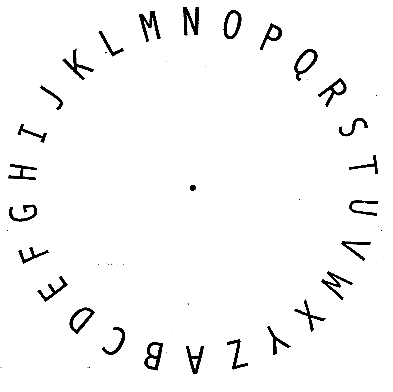
\includegraphics{caesar_large.png}
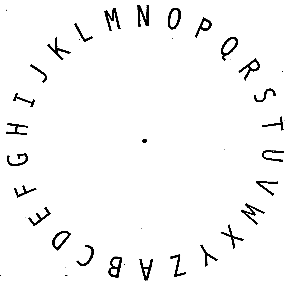
\includegraphics{caesar_small.png}
\end{center}

\chapter{Frequency table}
\label{app:frequencies}
This table gives letter frequency percentages for long English texts.

\begin{center}
\begin{tabular}{ccccccccccccc}
A & B & C & D & E & F & G & H & I & J & K & L & M \\
8.2 & 1.5 & 2.8 & 4.3 & 12.7 & 2.2 & 2.0 & 6.1 & 7.0 & 0.2 & 0.8 & 4.0 & 2.4 \\
\\
N & O & P & Q & R & S & T & U & V & W & X & Y & Z \\
6.7 & 7.5 & 1.9 & 0.1 & 6.0 & 6.3 & 9.1 & 2.8 & 1.0 & 2.4 & 0.2 & 2.0 & 0.1
\end{tabular}
\end{center}

\chapter{Vigen\`{e}re square}
\label{app:square}
\begin{center}
\begin{tikzpicture}
\foreach \i in {0,...,25} {
  \foreach \j in {0,...,25} {
    \edef\k{\ifnum\numexpr\i+\j\relax>25
        \the\numexpr\i+\j-26\relax
      \else
        \the\numexpr\i+\j\relax
      \fi}
  \node[draw,minimum size=0.5cm,inner sep=0pt]
    at (\i*0.5,-\j*0.5) {\strut\texttt{\symbol{\numexpr`A+\k\relax}}};
  }
  \node at (-0.5,-\i*0.5) {\strut\i};
  \node at (\i*0.5,0.5)   {\strut\i};
}
\end{tikzpicture}
\end{center}

\chapter{Frequency tables for Vigen\`{e}re exercises}
\begin{table}[H]
\begin{center}
\begin{tabular}{c|ccccc}
Letter & 1 & 2 & 3 & 4 & 5 \\
\hline
\ciphertext{A} & 1.9 & 1.9 & 5.7 & 1.9 & 0.0 \\
\ciphertext{B} & 3.8 & 3.8 & 13.2 & 7.5 & 0.0 \\
\ciphertext{C} & 5.7 & 0.0 & 11.3 & 1.9 & 1.9 \\
\ciphertext{D} & 7.5 & 0.0 & 0.0 & 0.0 & 0.0 \\
\ciphertext{E} & 3.8 & 0.0 & 1.9 & 11.3 & 5.7 \\
\ciphertext{F} & 0.0 & 0.0 & 1.9 & 11.3 & 1.9 \\
\ciphertext{G} & 3.8 & 0.0 & 9.4 & 13.2 & 3.8 \\
\ciphertext{H} & 3.8 & 7.5 & 11.3 & 5.7 & 3.8 \\
\ciphertext{I} & 17.0 & 1.9 & 5.7 & 0.0 & 9.4 \\
\ciphertext{J} & 1.9 & 3.8 & 3.8 & 0.0 & 1.9 \\
\ciphertext{K} & 0.0 & 3.8 & 1.9 & 0.0 & 0.0 \\
\ciphertext{L} & 1.9 & 18.9 & 0.0 & 3.8 & 5.7 \\
\ciphertext{M} & 0.0 & 5.7 & 0.0 & 0.0 & 9.4 \\
\ciphertext{N} & 0.0 & 0.0 & 0.0 & 1.9 & 0.0 \\
\ciphertext{O} & 0.0 & 3.8 & 1.9 & 0.0 & 0.0 \\
\ciphertext{P} & 9.4 & 9.4 & 1.9 & 0.0 & 3.8 \\
\ciphertext{Q} & 1.9 & 0.0 & 5.7 & 1.9 & 1.9 \\
\ciphertext{R} & 0.0 & 0.0 & 5.7 & 20.8 & 5.7 \\
\ciphertext{S} & 5.7 & 5.7 & 5.7 & 0.0 & 5.7 \\
\ciphertext{T} & 18.9 & 0.0 & 3.8 & 1.9 & 1.9 \\
\ciphertext{U} & 5.7 & 5.7 & 0.0 & 3.8 & 0.0 \\
\ciphertext{V} & 1.9 & 15.1 & 0.0 & 9.4 & 11.3 \\
\ciphertext{W} & 3.8 & 3.8 & 5.7 & 0.0 & 13.2 \\
\ciphertext{X} & 3.8 & 0.0 & 1.9 & 0.0 & 11.3 \\
\ciphertext{Y} & 0.0 & 9.4 & 0.0 & 1.9 & 1.9 \\
\ciphertext{Z} & 0.0 & 1.9 & 3.8 & 1.9 & 0.0
\end{tabular}
\caption{Frequency table for Vigen\`{e}re exercise \ref{exer:vig:preamble}}
\label{app:vig:preamble}
\end{center}
\end{table}

\begin{table}[H]
\begin{center}
\begin{tabular}{c|cccc}
Letter & 1 & 2 & 3 & 4 \\
\hline
\ciphertext{A} & 6.4 & 4.3 & 0.0 & 4.3 \\
\ciphertext{B} & 0.0 & 10.6 & 2.1 & 0.0 \\
\ciphertext{C} & 10.6 & 6.4 & 0.0 & 4.3 \\
\ciphertext{D} & 2.1 & 8.5 & 12.8 & 0.0 \\
\ciphertext{E} & 2.1 & 0.0 & 0.0 & 6.4 \\
\ciphertext{F} & 6.4 & 8.5 & 2.1 & 0.0 \\
\ciphertext{G} & 10.6 & 4.3 & 6.4 & 2.1 \\
\ciphertext{H} & 2.1 & 2.1 & 6.4 & 10.6 \\
\ciphertext{I} & 6.4 & 4.3 & 2.1 & 17.0 \\
\ciphertext{J} & 4.3 & 0.0 & 2.1 & 0.0 \\
\ciphertext{K} & 4.3 & 2.1 & 0.0 & 4.3 \\
\ciphertext{L} & 0.0 & 0.0 & 8.5 & 2.1 \\
\ciphertext{M} & 2.1 & 2.1 & 0.0 & 0.0 \\
\ciphertext{N} & 4.3 & 0.0 & 0.0 & 0.0 \\
\ciphertext{O} & 0.0 & 10.6 & 6.4 & 0.0 \\
\ciphertext{P} & 2.1 & 0.0 & 4.3 & 4.3 \\
\ciphertext{Q} & 8.5 & 2.1 & 14.9 & 6.4 \\
\ciphertext{R} & 8.5 & 2.1 & 10.6 & 12.8 \\
\ciphertext{S} & 0.0 & 12.8 & 0.0 & 8.5 \\
\ciphertext{T} & 4.3 & 2.1 & 2.1 & 4.3 \\
\ciphertext{U} & 2.1 & 2.1 & 12.8 & 0.0 \\
\ciphertext{V} & 6.4 & 4.3 & 2.1 & 4.3 \\
\ciphertext{W} & 6.4 & 12.8 & 2.1 & 0.0 \\
\ciphertext{X} & 0.0 & 0.0 & 0.0 & 6.4 \\
\ciphertext{Y} & 2.1 & 0.0 & 4.3 & 2.1 \\
\ciphertext{Z} & 0.0 & 0.0 & 0.0 & 0.0
\end{tabular}
\caption{Frequency table for Vigen\`{e}re exercise \ref{exer:vig:raven}}
\label{app:vig:raven}
\end{center}
\end{table}

\begin{table}[H]
\begin{center}
\begin{tabular}{c|ccc}
Letter & 1 & 2 & 3 \\
\hline
\ciphertext{A} & 0.9 & 4.5 & 8.2 \\
\ciphertext{B} & 5.5 & 0.0 & 0.9 \\
\ciphertext{C} & 7.3 & 0.9 & 4.5 \\
\ciphertext{D} & 0.0 & 3.6 & 3.6 \\
\ciphertext{E} & 0.0 & 7.3 & 16.4 \\
\ciphertext{F} & 2.7 & 8.2 & 0.9 \\
\ciphertext{G} & 0.0 & 6.4 & 0.0 \\
\ciphertext{H} & 9.1 & 3.6 & 12.7 \\
\ciphertext{I} & 8.2 & 0.9 & 3.6 \\
\ciphertext{J} & 0.9 & 2.7 & 0.0 \\
\ciphertext{K} & 0.9 & 5.5 & 0.0 \\
\ciphertext{L} & 7.3 & 13.6 & 2.7 \\
\ciphertext{M} & 9.1 & 0.9 & 0.9 \\
\ciphertext{N} & 8.2 & 0.0 & 4.5 \\
\ciphertext{O} & 4.5 & 3.6 & 10.0 \\
\ciphertext{P} & 0.9 & 0.0 & 3.6 \\
\ciphertext{Q} & 0.9 & 0.0 & 0.0 \\
\ciphertext{R} & 0.0 & 0.0 & 2.7 \\
\ciphertext{S} & 0.9 & 6.4 & 5.5 \\
\ciphertext{T} & 0.0 & 0.0 & 11.8 \\
\ciphertext{U} & 9.1 & 4.5 & 2.7 \\
\ciphertext{V} & 0.9 & 1.8 & 1.8 \\
\ciphertext{W} & 2.7 & 15.5 & 1.8 \\
\ciphertext{X} & 4.5 & 2.7 & 0.0 \\
\ciphertext{Y} & 13.6 & 0.9 & 0.9 \\
\ciphertext{Z} & 1.8 & 6.4 & 0.0
\end{tabular}
\caption{Frequency table for Vigen\`{e}re exercise \ref{exer:vig:declaration}}
\label{app:vig:declaration}
\end{center}
\end{table}

\begin{table}[H]
\begin{center}
\begin{tabular}{c|ccccc}
Letter & 1 & 2 & 3 & 4 & 5 \\
\hline
\ciphertext{A} & 0.0 & 7.7 & 0.0 & 0.0 & 10.3 \\
\ciphertext{B} & 0.0 & 0.0 & 0.0 & 5.1 & 7.7 \\
\ciphertext{C} & 0.0 & 0.0 & 7.7 & 7.7 & 0.0 \\
\ciphertext{D} & 0.0 & 5.1 & 5.1 & 0.0 & 0.0 \\
\ciphertext{E} & 10.3 & 10.3 & 15.4 & 0.0 & 5.1 \\
\ciphertext{F} & 7.7 & 0.0 & 12.8 & 10.3 & 10.3 \\
\ciphertext{G} & 2.6 & 7.7 & 2.6 & 0.0 & 7.7 \\
\ciphertext{H} & 5.1 & 2.6 & 0.0 & 12.8 & 5.1 \\
\ciphertext{I} & 2.6 & 5.1 & 5.1 & 10.3 & 2.6 \\
\ciphertext{J} & 0.0 & 0.0 & 2.6 & 0.0 & 2.6 \\
\ciphertext{K} & 2.6 & 0.0 & 5.1 & 2.6 & 0.0 \\
\ciphertext{L} & 2.6 & 2.6 & 2.6 & 0.0 & 2.6 \\
\ciphertext{M} & 5.1 & 5.1 & 0.0 & 2.6 & 0.0 \\
\ciphertext{N} & 15.4 & 7.7 & 5.1 & 0.0 & 7.7 \\
\ciphertext{O} & 20.5 & 7.7 & 0.0 & 5.1 & 0.0 \\
\ciphertext{P} & 0.0 & 0.0 & 5.1 & 0.0 & 2.6 \\
\ciphertext{Q} & 0.0 & 0.0 & 0.0 & 0.0 & 2.6 \\
\ciphertext{R} & 0.0 & 2.6 & 10.3 & 7.7 & 10.3 \\
\ciphertext{S} & 2.6 & 5.1 & 0.0 & 5.1 & 0.0 \\
\ciphertext{T} & 12.8 & 5.1 & 0.0 & 2.6 & 5.1 \\
\ciphertext{U} & 5.1 & 10.3 & 0.0 & 5.1 & 2.6 \\
\ciphertext{V} & 2.6 & 5.1 & 15.4 & 0.0 & 5.1 \\
\ciphertext{W} & 5.1 & 2.6 & 0.0 & 12.8 & 2.6 \\
\ciphertext{X} & 0.0 & 0.0 & 2.6 & 0.0 & 5.1 \\
\ciphertext{Y} & 0.0 & 10.3 & 5.1 & 0.0 & 0.0 \\
\ciphertext{Z} & 0.0 & 0.0 & 0.0 & 10.3 & 2.6
\end{tabular}
\caption{Frequency table for Vigen\`{e}re exercise \ref{exer:vig:astley}}
\label{app:vig:astley}
\end{center}
\end{table}

\chapter{Modular inverses}
\label{app:inverses}
\begin{center}
\def\arraystretch{1.5}
\begin{tabular}{|c|c|c|c|c|c|c|c|c|c|c|c|c|c|c|}
\hline
$n$ & 1 & 2 & 3 & 4 & 5 & 6 & 7 & 8 & 9 & 10 & 11 & 12 & 13 & 14 \\
\hline
$n^{-1} \mod 29$ & & & & & & & & & & & & & & \\
\hline
$n$ & 15 & 16 & 17 & 18 & 19 & 20 & 21 & 22 & 23 & 24 & 25 & 26 & 27 & 28 \\
\hline
$n^{-1} \mod 29$ & & & & & & & & & & & & & & \\
\hline
\end{tabular}
\def\arraystretch{1.0}
\end{center}

\chapter{Enigma simulator}
\label{app:enigma}
The following three pages contain a paper Enigma simulator. To assemble it, follow these steps:
\begin{enumerate}
\item On the first page, cut the three dashed lines near the top and bottom of the page, as well as the two dashed lines at the left of the page.
\item On the second and third pages, cut out the three alphabet strips and four plugboards on each page along the dotted lines.
\item Match the alphabet strips by number. For each set of strips, cover the tab at the top of the strip from the third page (marked ``link") with the bottom of the corresponding strip from the second page; apply clear tape. When finished, each strip will have a tab at the top and bottom, with a shaded line in the middle, to form an uninterrupted set of letters.
\end{enumerate}

To set the simulator, follow these steps:
\begin{enumerate}
\item Choose a plugboard. Insert the plugboard into the two slots at the left of the simulator.
\item Choose a rotor order. Insert the three rotor strips into the corresponding slots.
\item Choose an initial rotor orientation. For each rotor, move the shaded line so it lines up with the desired letter to its left.
\end{enumerate}

To encrypt or decrypt a message after the simulator is set, follow these steps:
\begin{enumerate}
\item If the letter appears on the plugboard, swap it with the listed letter.
\item Find this letter in the list to the left of the first rotor. Follow it into the first rotor and find the matching letter on the right of the rotor.
\item Exit the first rotor and enter directly into the second. Find the matching letter on the right of the rotor.
\item Exit the second rotor and enter directly into the third. Find the matching letter on the right of the rotor.
\item Exit the third rotor to the reflector. Determine the reflected letter.
\item Go through the rotors again, this time in reverse order.
\item Apply the plugboard if needed after the first rotor.
\item Move the first rotor down one letter. If the gray strip was already at the bottom letter, move it to the top and move the second rotor down one letter. If its gray strip was already at the bottom letter, move it to the top and move the third rotor down one letter. If its gray strip was already at the bottom letter, move it to the top.
\item Repeat these steps for each letter of the message.
\end{enumerate}

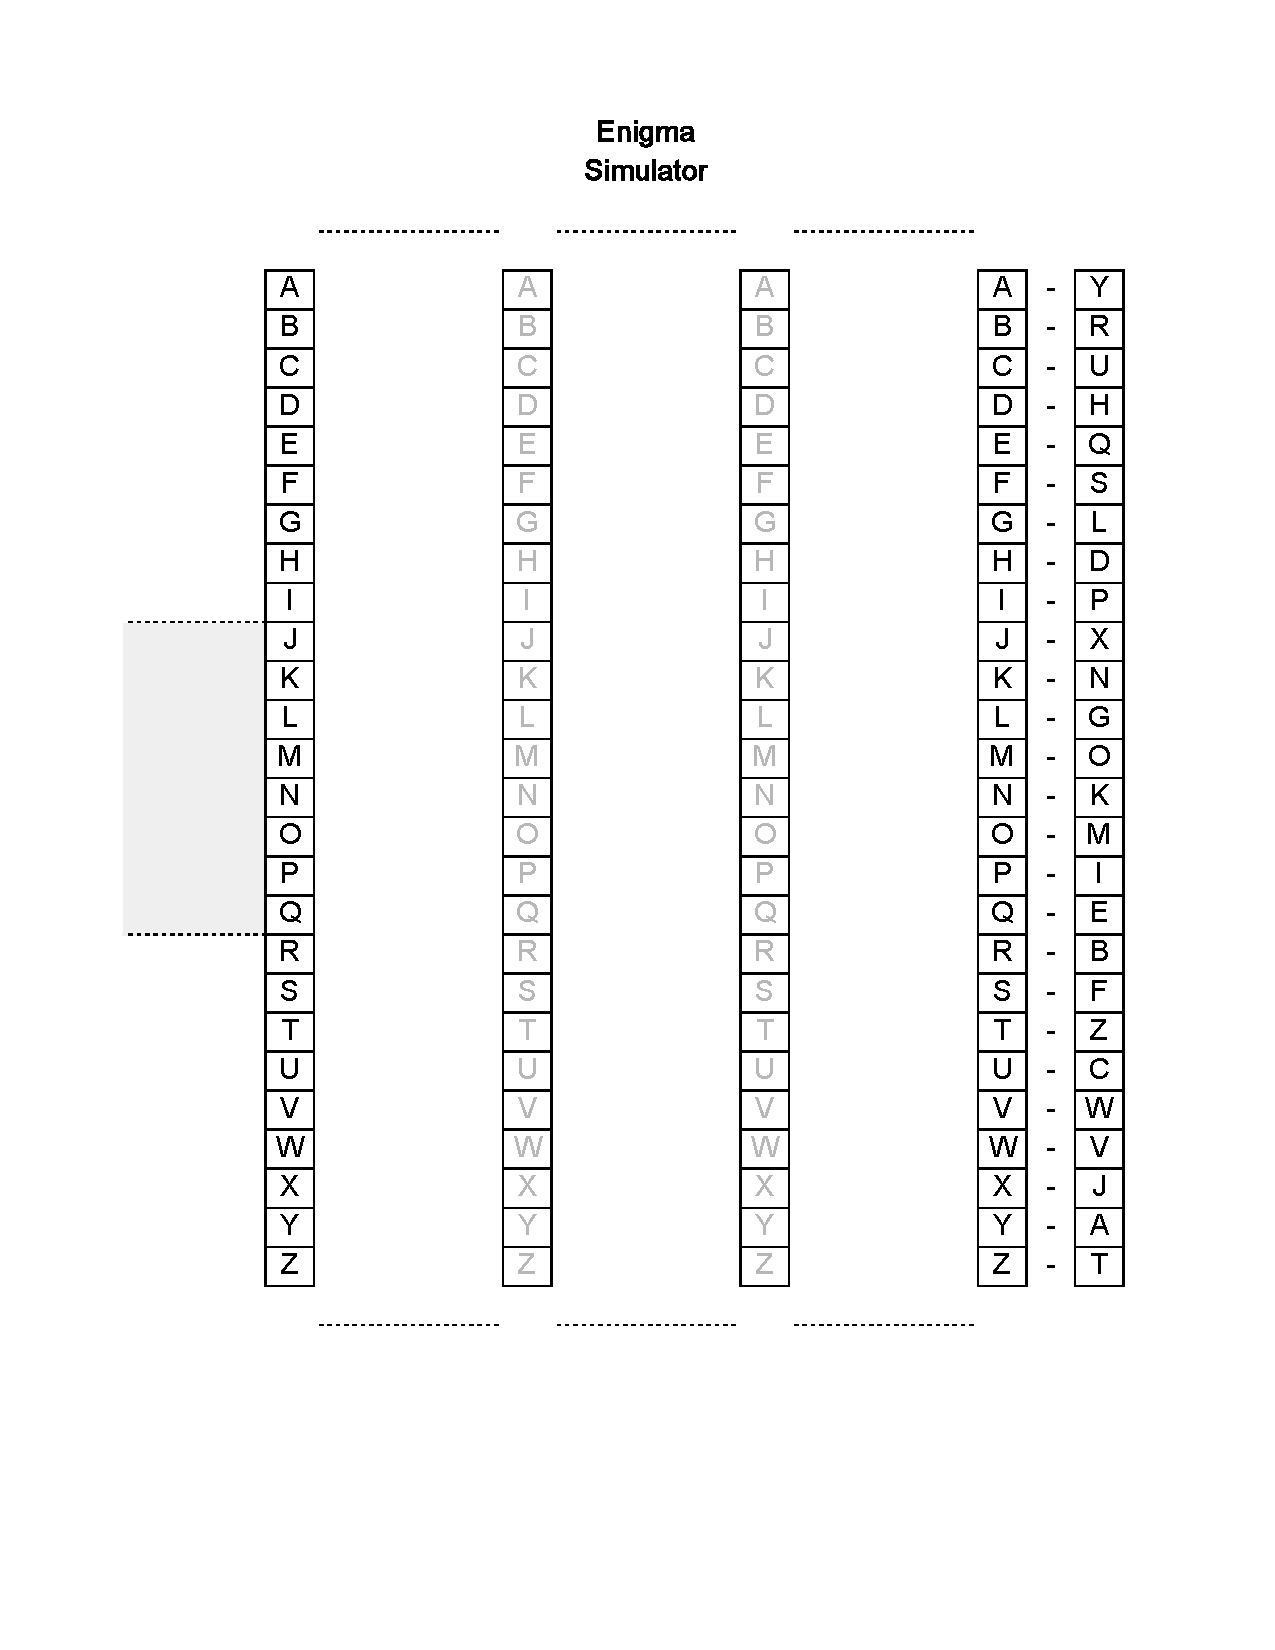
\includepdf[pages={-}]{simulator.pdf}

\chapter{Letter encoding}
\label{app:encoding}
\def\arraystretch{1.3}
\rowcolors{2}{gray!25}{white}

\begin{center}
\begin{tabular}{cccc}
Letter & $a \mod 29$ & Binary & $a^{-1} \mod 29$ \\
\hline
\texttt{A}  & \texttt{0}  & \texttt{00000} & -- \\
\texttt{B}  & \texttt{1}  & \texttt{00001} & \texttt{1} \\
\texttt{C}  & \texttt{2}  & \texttt{00010} & \texttt{15} \\
\texttt{D}  & \texttt{3}  & \texttt{00011} & \texttt{10} \\
\texttt{E}  & \texttt{4}  & \texttt{00100} & \texttt{22} \\
\texttt{F}  & \texttt{5}  & \texttt{00101} & \texttt{6} \\
\texttt{G}  & \texttt{6}  & \texttt{00110} & \texttt{5} \\
\texttt{H}  & \texttt{7}  & \texttt{00111} & \texttt{25} \\
\texttt{I}  & \texttt{8}  & \texttt{01000} & \texttt{11} \\
\texttt{J}  & \texttt{9}  & \texttt{01001} & \texttt{13} \\
\texttt{K}  & \texttt{10} & \texttt{01010} & \texttt{3} \\
\texttt{L}  & \texttt{11} & \texttt{01011} & \texttt{8} \\
\texttt{M}  & \texttt{12} & \texttt{01100} & \texttt{17} \\
\texttt{N}  & \texttt{13} & \texttt{01101} & \texttt{9} \\
\texttt{O}  & \texttt{14} & \texttt{01110} & \texttt{27} \\
\texttt{P}  & \texttt{15} & \texttt{01111} & \texttt{2} \\
\texttt{Q}  & \texttt{16} & \texttt{10000} & \texttt{20} \\
\texttt{R}  & \texttt{17} & \texttt{10001} & \texttt{12} \\
\texttt{S}  & \texttt{18} & \texttt{10010} & \texttt{21} \\
\texttt{T}  & \texttt{19} & \texttt{10011} & \texttt{26} \\
\texttt{U}  & \texttt{20} & \texttt{10100} & \texttt{16} \\
\texttt{V}  & \texttt{21} & \texttt{10101} & \texttt{18} \\
\texttt{W}  & \texttt{22} & \texttt{10110} & \texttt{4} \\
\texttt{X}  & \texttt{23} & \texttt{10111} & \texttt{24} \\
\texttt{Y}  & \texttt{24} & \texttt{11000} & \texttt{23} \\
\texttt{Z}  & \texttt{25} & \texttt{11001} & \texttt{7} \\
\texttt{\_} & \texttt{26} & \texttt{11010} & \texttt{19} \\
\texttt{,}  & \texttt{27} & \texttt{11011} & \texttt{14} \\
\texttt{.}  & \texttt{28} & \texttt{11100} & \texttt{28} \\
\rowcolor{gray!50}
\texttt{?}  & \texttt{29} & \texttt{11101} & -- \\
\rowcolor{gray!50}
\texttt{/}  & \texttt{30} & \texttt{11110} & -- \\
\rowcolor{gray!50}
\texttt{'}  & \texttt{31} & \texttt{11111} & -- \\
\end{tabular}
\end{center}

\chapter{List of activities}
\section{Random number generation}
The goal of this activity is to examine the difference between random number generation and pseudorandom number generation. Split into two teams. Each team first writes down a ``random" list of 20 Hs and Ts, in any order, on a sheet of paper. The team then flips a coin 20 times and writes down the resulting Hs and Ts (for heads and tails, respectively) on an indentical sheet of paper. It may be useful to further split the team into groups, each armed with a coin, to complete a portion of the flips.

When both teams have their two lists, they exchange them without knowing which list is from the coin flips and which is from the made-up flips. The teams must try to guess which is which. The teams should list what qualities of each list led them to their choice.

\section{Combinatorics of the SET card game}
The goal of this activity is to understand the application of combinatorics to the SET card game. Split into groups of about five people each. Each groups needs a copy of the SET card game. Play a few rounds of the game to get a sense of the patterns that you find in the cards. Then answer the following questions:
\begin{enumerate}
\item The SET card game includes cards with every possible combination of number, shape, shading, and color. How many cards are there? How do you obtain this number? \solution{There are $3^4=81$ cards.}
\item Suppose you draw two cards at random from the SET deck. Is it always possible to find a third card to complete a SET? How many such SETs exist for two given cards? \solution{There is exactly one card that completes the SET.}
\item Suppose you draw one card at random from the SET deck. Is it always possible to find two additional cards to complete a SET? How many such SETs exist for a given card? \solution{It is always possible. There are $80$ ways to draw a second card, and only one way to draw the final card. However, overcounting means there are $40$ such SETs.}
\item How many cards do you think can be dealt such that no SET appears among them? This is a very difficult problem, so make an educated estimate. \solution{It is possible to deal $20$ cards such that no SET is present.}
\end{enumerate}

\section{Tower of Hanoi}
The goal of this activity is to understand principles of counting and recursion. In the Tower of Hanoi puzzle, there are three pegs in a row. On the left peg are $n$ disks of decreasing size arranged in a pyramid; that is, the disks get smaller in size from bottom to top. The goal of the puzzle is to move all disks to the right peg, one at a time. A legal move consists of moving the top disk from any peg to any other peg, as long as no disk ever sits on top of a smaller one. Let $h_n$ denote the fewest number of moves required to solve the Tower of Hanoi problem with $n$ disks.
\begin{enumerate}
\item Find $h_1$, $h_2$, $h_3$, and $h_4$. \solution{The numbers are $h_1 = 1$, $h_2 = 3$, $h_3 = 7$, and $h_4 = 15$.}
\item Develop a recursive formula that establishes $h_n$ in terms of $h_{n-1}$; that is, if you know the fewest number of moves to solve the $(n-1)$-disk Tower of Hanoi problem, can you use this to figure out the fewest number of moves to solve the $n$-disk problem? It is not necessary to actually determine a formula for $h_{n-1}$ in this case! \solution{We have $h_n = 2h_{n-1} + 1$ since we first move the top $n-1$ disks to the middle peg in $h_{n-1}$ moves, then move the bottom disk to the right peg in one move, and then move the top $n-1$ disks to the right peg in $h_{n-1}$ moves.}
\item Hypothesize an explicit formula for $h_n$ that is not recursive. \solution{The formula is $h_n = 2^n - 1$.}
\end{enumerate}

\section{Measuring hash functions}
One common statistical requirement for a good hash function is that a change of a single bit of the input changes about half of the bits in the hash. This activity investigates whether modern hash functions obey this principle.

We will check to see if changing a single input bit to an MD5 hash results in a change of about half of the output bits. We will use the following:

\begin{center}
\begin{tabular}{cl}
& MD5 hexadecimal hash \\
\hline
Moors & \texttt{1CA29DFB8B94B8C082DAA4BAA2BC8B03} \\
Moops & \texttt{4BB03083EF11974A0CE92AD241C2F455}
\end{tabular}
\end{center}

\begin{enumerate}
\item We will examine only the last 32 bits of each hash. For each hash, write the hexadecimal digits we need to use to obtain these 32 bits. \solution{Since four bits correspond to a hexadecimal digit, we need eight digits of each hash, giving \texttt{A2BC8B03} and \texttt{41C2F455}.}
\item Write each of these smaller hexadecimal numbers in binary. \solution{\texttt{A2BC8B03 = 10100010 10111100 10001011 00000011}$_2$ \\ \texttt{41C2F455 = 01000001 11000010 11110100 01010101}$_2$}
\item In how many bits do these numbers differ? Is it close to half? \solution{They differ in 22 bits. This is about $60\%$ of the bits.}
\item What are some reasons why the two numbers might not differ in exactly half of the bits? \solution{We only checked a portion of the hash bits; the words we chose are not very long; the ``half of all bits" principle is statistical, not absolute.}
\end{enumerate}

We will investigate the same two words using the SHA-1 hash function.

\begin{center}
\begin{tabular}{cl}
& SHA-1 hexadecimal hash \\
\hline
Moors & \texttt{4B02EE525EDCF52B16F20C88A77BC8A0FAD3EAF1} \\
Moops & \texttt{669FC0C24C6061AC8EBF4A3C60AFC130E82296C4}
\end{tabular}
\end{center}

\begin{enumerate}
\item We will examine only the last 32 bits of each hash. For each hash, write the hexadecimal digits we need to use to obtain these 32 bits. \solution{We use \texttt{FAD3EAF1} and \texttt{E82296C4}.}
\item Write each of these smaller hexadecimal numbers in binary. \solution{\texttt{FAD3EAF1 = 11111010 11010011 11101010 11110001}$_2$ \\ \texttt{E82296C4 = 11101000 00100010 10010110 11000100}$_2$}
\item In how many bits do these numbers differ? Is it close to half? \solution{They differ in $16$ bits. This is exactly half of the bits.}
\end{enumerate}

We will investigate the same two words using the SHA-2 hash function.

\begin{center}
\begin{tabular}{cl}
& SHA-2 hexadecimal hash \\
\hline
Moors & \texttt{3C75C1374380D709E46B1E5CE82DFCDDD7F31D91DFD47AE42874A3585F0CF7A7} \\
Moops & \texttt{97756326C7366D99D7AD18446FE1ABF468A5B14D11FEC5A29AE1211E5DE6E34E}
\end{tabular}
\end{center}

\begin{enumerate}
\item We will examine only the last 32 bits of each hash. For each hash, write the hexadecimal digits we need to use to obtain these 32 bits. \solution{We use \texttt{5F0CF7A7} and \texttt{5DE6E34E}.}
\item Write each of these smaller hexadecimal numbers in binary. \solution{\texttt{5F0CF7A7 = 01011111 00001100 11110111 10100111}$_2$ \\ \texttt{5DE6E34E = 01011101 11100110 11100011 01001110}$_2$}
\item In how many bits do these numbers differ? Is it close to half? \solution{They differ in $13$ bits. This is about $40\%$ of the bits.}
\end{enumerate}

We will investigate the same two words using the SHA-3 hash function.

\begin{center}
\begin{tabular}{cl}
& SHA-3 hexadecimal hash \\
\hline
Moors & \texttt{E8B46458C7DD6771CAECA7C4B024C654AFFD7096B2C281702D2B5C231BD87A0D} \\
Moops & \texttt{429246D7D0B91819401DF7AEC1B74C75D94F7E7430BBE0ACD4077C1F23F2A322}
\end{tabular}
\end{center}

\begin{enumerate}
\item We will examine only the last 32 bits of each hash. For each hash, write the hexadecimal digits we need to use to obtain these 32 bits. \solution{We use \texttt{1BD87A0D} and \texttt{23F2A322}.}
\item Write each of these smaller hexadecimal numbers in binary.
\item In how many bits do these numbers differ? Is it close to half?
\end{enumerate}

\section{Secret sharing game}
The purpose of this activity is to learn to use the mathematical tools needed in polynomial secret sharing. Scrooge McDuck has locked a great treasure in his vault with a six-digit combination. Because he does not want any one person (or duck) to have any of the digits, he has used a polynomial scheme to distribute the digits.

\subsection{Equipment}
A total of 27 cards in six colors. Each color is labeled with a polynomial degree, and each card has an ordered pair:
\begin{itemize}
\item Red, $y=x^2-2x+3$: $(1,2),(-3,18),(4,11),(-2,11),(-1,6)$
\item Orange, $y=8x-4$: $(3,20),(-2,-20),(1,4),(9,68)$
\item Yellow, $y=-2x^2-2$: $(1,-4),(2,-10),(-1,-4),(-2,-10),(3,-20)$
\item Green, $y=-3x+9$: $(7,-12),(-3,18),(10,-21),(3,0)$
\item Blue, $y=2x^2-6x+4$: $(1,0),(2,0),(-1,12),(-2,24),(3,4)$
\item Purple, $y=15$: $(19,15),(-4,15),(12,15),(-1,15)$
\end{itemize}

\subsection{Rules}
\begin{itemize}
\item Divide into groups of two. If there are not enough cards to distribute evenly, remove some cards as needed. There must be at least three red, yellow, and blue cards; there must be at least two orange, green, and purple cards.
\item Shuffle the deck and deal all the cards.
\item On group A's turn, they can either trade information or guess a digit.
\item If group A chooses to trade information, they ask any particular group B if group B has a specific color. If group B does, they choose one of these cards to give to group A; at the same time, group A chooses any card to give to group B and the turn ends. If group B does not have any cards of the given color, the turn ends.
\item If instead group A chooses to guess a digit of the combination, they write down the color and their guess for the instructor in secret. If the guess is correct, the turn ends. If the guess is incorrect, the turn ends and group A loses their next turn.
\item Play continues to the next group clockwise.
\item The game ends when any group guesses all six digits in the combination.
\end{itemize}

\chapter{Research projects}
Here are several prompts for research.
\begin{enumerate}
\item For either the United States, India, Germany, or the United Kingdom, write an essay on the history of public policy restricting encryption techniques in that country. Be sure to include an analysis of current policy.
\item Some argue that because encryption technologies can be used by criminals for illegal purposes, they should be regulated by governments. Others argue that principles of free speech require the free use of such technologies. Analyze both arguments and reach your own conclusion about which argument, if either, is correct. Be sure to justify any claims that you make in your discussion.
\item Recent news about information leaked to the press by former United States National Security Agency (NSA) contractor Edward Snowden details NSA efforts to persuade the security firm RSA to include a weakened algorithm in its suite of security products. Research this story and report on your findings.
\item A massive shift in cryptographic technology occurred with the introduction of public-key cryptography. Investigate recent cryptographic developments and speculate about what the next such shift might be.
\item Services like Dropbox, Microsoft SkyDrive and Google Drive allow users to store files on servers owned by those companies. Users' web connections to those services are typically encrypted, but the files themselves are not. Research and discuss the benefits and drawbacks of this arrangement. Suggest improvements that could solve some of the associated problems.
\item The encrypted email service Lavabit has been in the news recently because of United States National Security Agency (NSA) efforts to obtain encryption key information from the company. Research this story and report on your findings. Discuss the possible implications of the actions taken by the NSA and Lavabit.
\item Originally, email messages were sent from the sender to the recipient unencrypted. Efforts have since been taken to secure the contents of email messages in transit. Research the history of email security technologies and report your findings. Be sure to discuss the current state of email security and comment on recent and ongoing developments.
\item It is not uncommon for researchers to discover flaws in cryptographic algorithms or technologies that render them unsafe to use. Research an example of this and report your findings. Be sure to include a discussion of the algorithm or technology, the flaws that were found, and the impact of the announcement.
\item Investigate the history of hash collisions, focusing particularly on the MD5 hash. Report your findings.
\item Because companies and industries often invest heavily in particular cryptographic technologies, they are sometimes slow to update when better technologies are developed. Find an example of this and report your findings.
\end{enumerate}

\bibliographystyle{plain}
\nocite{*}
\bibliography{references}
\end{document}
